\section{Introduction} 

La deuxième release vise l’enrichissement et la finalisation technique de la plateforme . Elle est réalisée à travers trois sprints :
\begin{itemize}
    \item \textbf{Sprint 4 : Module AniMarket}
    \item \textbf{Sprint 5 : Module AniCare}
    \item \textbf{Sprint 6 : Conteneurisation, CI/CD, Déploiement et Monitoring}
\end{itemize}

\section{Sprint 4 : Module AniMarket}   
\begin{figure}[H]
    \centering
    
\includegraphics[width=3.5cm]{images/animarket.png}
    \caption{Logo du module AniMarket}
    \label{fig:logo-animarket}
\end{figure}
Ce sprint, d’une durée de \textbf{3 semaines}, est dédié au module AniMarket, permettant la gestion des annonces d’animaux (vente directe et enchères) et les interactions entre utilisateurs. 
\subsection{Sprint backlog}  
\begin{longtable}{|p{1cm}|p{5cm}|p{8cm}|p{1cm}|}
\caption{Sprint Backlog du Sprint 4}
\label{tab:sprint4-backlog} \\ 
\hline
\rowcolor{coloranimarket}
\textbf{ID} & \textbf{User Story} & \textbf{Tâches} & \textbf{Effort} \\
\hline
\endfirsthead

\hline
\rowcolor{coloranimarket}
\textbf{ID} & \textbf{User Story} & \textbf{Tâches} & \textbf{Effort} \\
\hline
\endhead

% ===================== US1 =====================
\multirow{5}{2cm}{US1}
& \multirow{5}{5cm}{En tant qu’utilisateur, je veux consulter la liste des animaux à vendre afin de découvrir les annonces disponibles}
& Conception de l’interface (Figma) & 1 j \\
\cline{3-4}
& & API récupération animaux & 1.5 j \\
\cline{3-4}
& & Interface enchères et ventes directes  & 1.5 j \\
\cline{3-4}
& & Filtrage , tri et recherche & 1 j \\
\cline{3-4}
& & Intégration frontend/backend & 1.5 j \\
\hline

% ===================== US2 =====================
\multirow{3}{2cm}{US2}
& \multirow{3}{5cm}{En tant qu’utilisateur, je veux proposer une offre sur une enchère}
& API offres et enchères & 1 j \\
\cline{3-4}
& & Intégration interface des offres & 1 j \\
\cline{3-4}
& & Tests & 0.5 j \\
\hline

% ===================== US3 =====================
\multirow{6}{2cm}{US3}
& \multirow{6}{5cm}{En tant qu’utilisateur, je veux gérer mes notifications afin d’être informé des interactions sur mes activités}
& Analyse besoins notifications & 1 j \\
\cline{3-4}
& & Développement microservice Notifications & 1.5 j \\
\cline{3-4}
& & Intégration RabbitMQ avec le microservice AniMarket et le microservice notifications & 1.5 j \\
\cline{3-4}
& & Création événements (offres, enchères, wishlist) & 1 j \\
\cline{3-4}
& & Interface notifications frontend & 1 j \\
\cline{3-4}
& & Marquer comme lu / non lu & 0.5 j \\
\hline

% ===================== US4 =====================
\multirow{4}{2cm}{US4}
& \multirow{4}{5cm}{En tant que vendeur, je veux gérer mes animaux à vendre afin de maintenir mes annonces à jour}
& API CRUD animaux & 1.5 j \\
\cline{3-4}
& & Interface espace animarket & 1 j \\
\cline{3-4}
& & Gestion des annonces (frontend) & 1 j \\
\cline{3-4}
& & Tests & 0.5 j \\
\hline

% ===================== US5 =====================
\multirow{3}{2cm}{US5}
& \multirow{3}{5cm}{En tant qu’utilisateur, je veux gérer ma wishlist}
& API wishlist & 1 j \\
\cline{3-4}
& & Ajout / suppression animal & 0.5 j \\
\cline{3-4}
& & Interface ma wishlist & 1 j \\
\hline

% ===================== US6 =====================
\multirow{3}{2cm}{US6}
& \multirow{3}{5cm}{En tant que vendeur, je veux gérer les offres reçues}
& API gestion offres & 1 j \\
\cline{3-4}
& & Accepter / refuser offre & 1 j \\
\cline{3-4}
& & Tests & 0.5 j \\
\hline

% ===================== US7 =====================
\multirow{3}{2cm}{US7}
& \multirow{3}{5cm}{En tant qu’utilisateur, je veux commenter et noter un animal}
& API commentaires et avis & 1 j \\
\cline{3-4}
& & Interface frontend & 1 j \\
\cline{3-4}
& & Tests & 0.5 j \\
\hline

% ===================== US8 =====================
\multirow{3}{2cm}{US8}
& \multirow{3}{5cm}{En tant qu’utilisateur, je veux discuter avec le vendeur}
& Analyse & 0.5 j \\
\cline{3-4}
& & Intégration bouton WhatsApp & 0.5 j \\
\cline{3-4}
& & Génération lien wa.me & 0.5 j \\
\hline

\end{longtable}
\newpage
\subsection{Diagramme des cas d’utilisation du sprint 4} 
Dans cette section, nous présentons le diagramme des cas d’utilisation du Sprint 4, dédié au module AniMarket.  
Ce diagramme illustre les principales interactions entre l’utilisateur et le système, notamment la gestion des annonces, des enchères et des ventes directes.  
La figure ci-dessous représente le diagramme des cas d’utilisation correspondant : 


\begin{figure}[H]
    \centering
  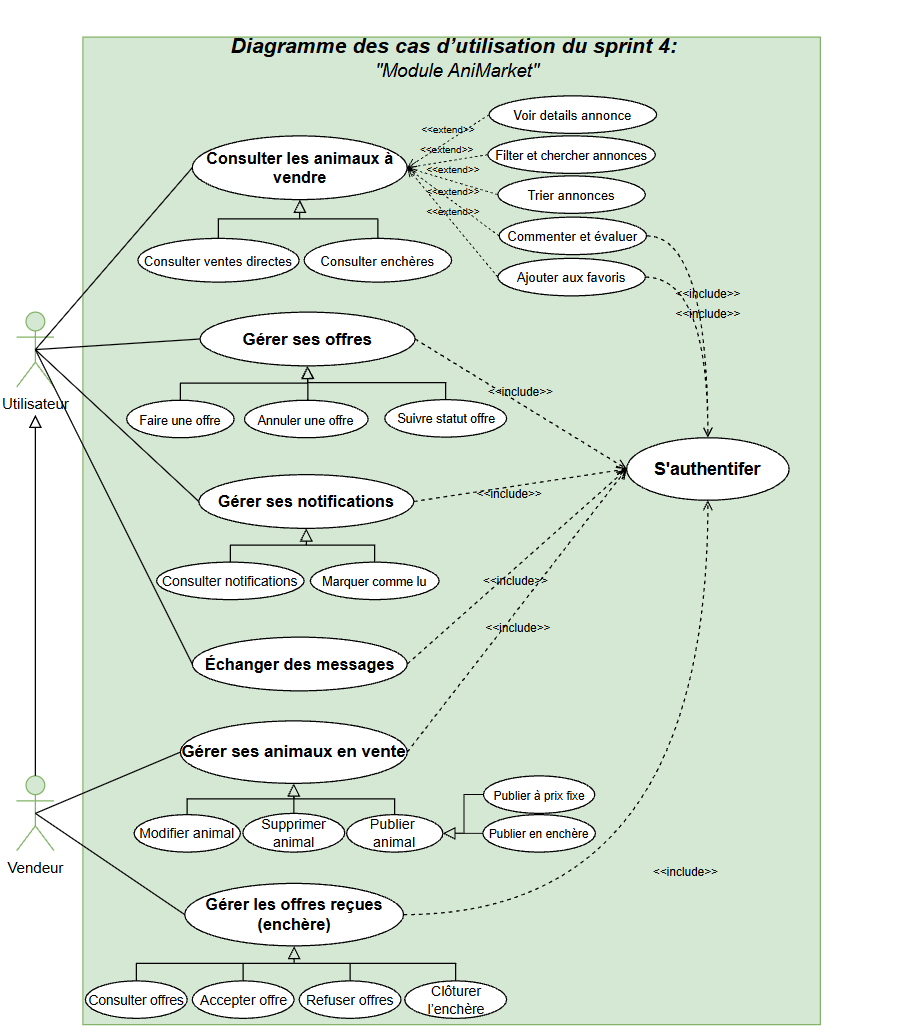
\includegraphics[width=0.98\linewidth, height=18.5cm, keepaspectratio]{images/usecase animarket.png}
    \caption{Diagramme des cas d’utilisation du sprint 4}
    \label{fig:usecase-sprint4}
\end{figure} 
\newpage
\subsection{Descriptions textuelles des cas d’utilisation du sprint 4}  
  Dans cette section, nous présentons les descriptions textuelles des cas d’utilisation du Sprint 4 afin de détailler le comportement du système pour chaque fonctionnalité du module AniMarket. 
  \subsubsection{Description textuelle du cas d’utilisation « Consulter les animaux à vendre (prix fixe ou enchères) »}

Le tableau ci-dessous illustre le cas d’utilisation Consulter les animaux à vendre, lors de la recherche et de la consultation des annonces disponibles (prix fixe ou enchères) :

\begin{longtable}{|c|p{11cm}|}
\caption{Description textuelle du cas d’utilisation "Consulter les animaux à vendre"}
\label{tab:consulter_animaux_vente} \\
\hline
\cellcolor{coloranimarket} \textbf{Nom du cas d'utilisation } & Consulter les animaux à vendre (prix fixe ou enchères) \\
\hline
\cellcolor{coloranimarket} \textbf{Acteurs} & Utilisateur \\
\hline
\cellcolor{coloranimarket} \textbf{Description } & Tout utilisateur peut consulter les annonces d’animaux disponibles à la vente directe ou aux enchères dans le module AniMarket. \\
\hline
\cellcolor{coloranimarket} \textbf{Pré-condition } &  Accès à la plateforme sans authentification requise. \\
\hline
\cellcolor{coloranimarket} \textbf{Post-condition } & L’utilisateur a consulté la liste des animaux à vendre. \\
\hline
\cellcolor{coloranimarket} \textbf{Scénario nominal } & 
\begin{enumerate} 

\item L’utilisateur accède à la plateforme AniHub.
\item L’utilisateur choisit le module AniMarket.
\item Le système redirige l’utilisateur vers la page d'acceuil du  module AniMarket.
\item L’utilisateur choisit entre « Vente directe » ou « Enchères ».
\item Le système affiche la liste des animaux correspondante.
\item L’utilisateur peut filtrer eyt chercher les annonces selon différents critères (prix , espèce , race ...).
\item Le système affiche les résultats filtrés.
\item L’utilisateur sélectionne une annonce.
\item Le système affiche les détails de l’annonce. 
\item L’utilisateur peut ajouter un animal à sa wishlist.
\item Le système ajoute l’animal à la wishlist de l’utilisateur.
\item L’utilisateur peut commenter et laisser un avis sur l’animal.
\item Le système enregistre le commentaire et l’avis de l’utilisateur.
\end{enumerate} \\
\hline
\end{longtable}

\newpage
\subsubsection{Description textuelle du cas d’utilisation « Gérer ses offres envoyées »}

Le tableau ci-dessous illustre le cas d’utilisation Gérer ses offres envoyées, permettant à l’utilisateur de faire et annuler une offre sur une enchère :
\begin{longtable}{|c|p{11cm}|}
\caption{Description textuelle du cas d’utilisation "Gérer ses offres envoyées"}
\label{tab:gerer_offres} \\
\hline
\cellcolor{coloranimarket} \textbf{Nom du cas d'utilisation } & Gérer ses offres envoyées \\
\hline
\cellcolor{coloranimarket} \textbf{Acteurs} & Utilisateur \\
\hline
\cellcolor{coloranimarket} \textbf{Description } & L’utilisateur peut consulter les offres d’une enchère, faire une nouvelle offre et annuler une offre déjà envoyée. \\
\hline
\cellcolor{coloranimarket} \textbf{Pré-condition } & L’utilisateur doit accéder aux détails d’une enchère. \\
\hline
\cellcolor{coloranimarket} \textbf{Post-condition } & Les offres sont ajoutées, supprimées avec succées. \\
\hline
\cellcolor{coloranimarket} \textbf{Scénario nominal } &
\begin{enumerate}
\item L’utilisateur accède à la plateforme AniHub.
\item L’utilisateur choisit le module AniMarket.
\item Le système redirige l’utilisateur vers la page d’accueil du module AniMarket.
\item L’utilisateur choisit la catégorie Enchères.
\item Le système affiche la liste des animaux en enchères.
\item L’utilisateur consulte les détails d’une enchère.
\item Selon l’action de l’utilisateur :

\begin{itemize}

\item \textbf{Cas 1 : Publication d’une offre}
\begin{enumerate}
\item L’utilisateur saisit un montant et envoie une offre.
\item Le système vérifie et enregistre l’offre.
\item Le système confirme l’envoi de l’offre.
\end{enumerate}


\item \textbf{Cas 2 : Suppression d’une offre}
\begin{enumerate}
\item Le système supprime l’offre et confirme l’annulation.
\item Si l’offre supprimée était la plus élevée, le système met à jour le prix de l’enchère.
\end{enumerate}

\end{itemize}

\end{enumerate} \\
\hline
\cellcolor{coloranimarket} \textbf{Scénario alternatif :} &
\begin{itemize}
\item Si l’utilisateur saisit une offre inférieure ou égale à la dernière offre, le système affiche une erreur.
\item Si l’utilisateur annule une offre qui n’est pas la plus élevée, le système supprime l’offre sans impact sur le prix actuel de l’enchère.
\end{itemize} \\
\hline
\end{longtable} 
\newpage 


\subsubsection{Description textuelle du cas d’utilisation « Gérer mes animaux à vendre »}
Le tableau ci-dessous illustre le cas d’utilisation « Gérer mes animaux à vendre » dans le module AniMarket :
\begin{longtable}{|c|p{11cm}|}
\caption{Description textuelle du cas d'utilisation "Gérer mes animaux à vendre"}
\label{tab:gerer_animaux_vente} \\
\hline
\cellcolor{coloranimarket}\textbf{Nom du cas d'utilisation } & Gérer mes animaux à vendre \\
\hline
\cellcolor{coloranimarket}\textbf{Acteurs} & Vendeur \\
\hline
\cellcolor{coloranimarket}\textbf{Description } & Le vendeur peut publier, modifier et supprimer ses annonces d’animaux dans AniMarket (vente directe ou enchères). \\
\hline
\cellcolor{coloranimarket}\textbf{Pré-condition } & L’utilisateur doit être authentifié en tant que vendeur. \\
\hline
\cellcolor{coloranimarket}\textbf{Post-condition } & Les annonces sont correctement publiées, mises à jour ou supprimées. \\
\hline

\cellcolor{coloranimarket}\textbf{Scénario nominal } &
\begin{enumerate}
\item L’utilisateur se connecte à son compte
\item L’utilisateur sélectionne le module AniMarket.
\item Le système redirige l’utilisateur vers AniMarket.
\item L’utilisateur accède à son <<espace animarket>>.
\item Le système affiche la liste de ses animaux à vendre.

\item \textbf{Cas publication :}
\begin{itemize}
\item L’utilisateur clique sur « Publier un animal ».
\item Le système affiche un formulaire de création.
\item L’utilisateur vente directe ou enchère,  saisit les informations et valide la publication.
\item Le système enregistre l’annonce et l’affiche.
\end{itemize}

\item \textbf{Cas modification :}
\begin{itemize}
\item L’utilisateur et clique sur « Modifier ».
\item Le système affiche le formulaire pré-rempli.
\item L’utilisateur modifie les informations.
\end{itemize}

\item \textbf{Cas suppression :}
\begin{itemize}
\item L’utilisateur clique sur « Supprimer ».
\item Le système demande confirmation.
\item L’utilisateur confirme la suppression.
\item Le système supprime l’annonce.
\end{itemize}

\item Le système met à jour et affiche un message de succès.
\end{enumerate} \\
\hline

\cellcolor{coloranimarket}\textbf{Scénario alternatif :} &
\begin{itemize}
\item En cas d’erreur lors de la publication ou modification, le système affiche un message d’erreur.
\item En cas d’annulation, l’annonce est conservée.
\end{itemize} \\
\hline

\end{longtable} 




\newpage 

\subsection{Diagramme des classes du sprint 4}  
Dans cette section, nous présentons le diagramme de classes du Sprint 4, qui regroupe l’ensemble des classes du module AniMarket.

La figure ci-dessous illustre le diagramme de classes correspondant :
\begin{figure}[H]
    \centering
    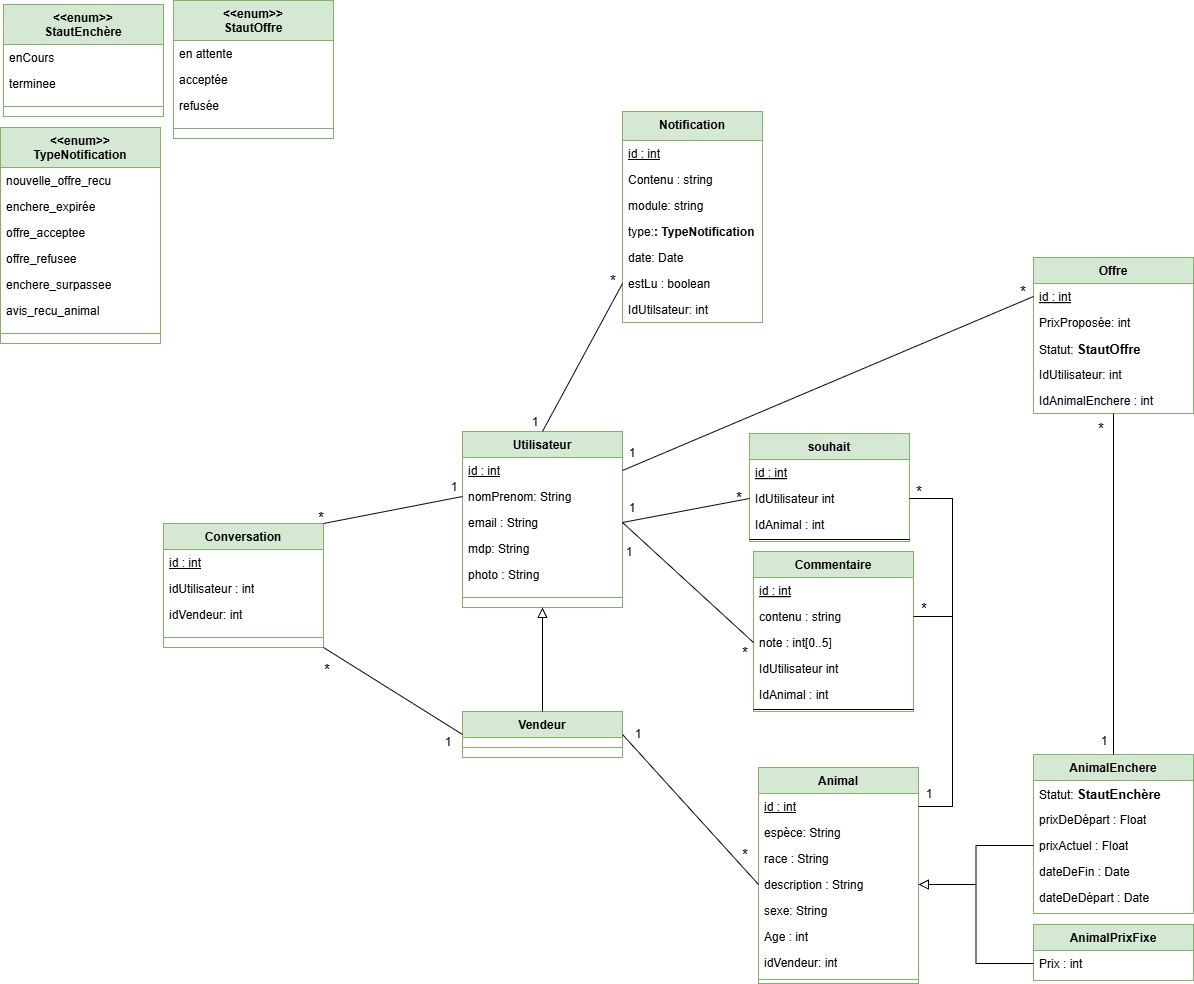
\includegraphics[width=1\textwidth, height=20cm, keepaspectratio]{images/class diagram animarket.png}
    \caption{Diagramme de classes du sprint 4}
    \label{fig:class_diagram_animarket}
\end{figure} 
\newpage 
\subsection{Diagrammes de séquence du sprint 4}

Dans cette section, nous présentons les diagrammes de séquence du quatrième sprint, illustrant les interactions entre les différents composants du système ainsi que le déroulement des principales fonctionnalités implémentées. 
\subsubsection{Diagramme de séquence : consultation des animaux à vendre}

Cette figure illustre les interactions de l’utilisateur avec le système pour consulter et filtrer les animaux disponibles à la vente, ainsi que les fonctionnalités associées telles que les commentaires, les favoris et l’envoi d’offres pour les enchères : 
\begin{figure}[H]
    \centering
    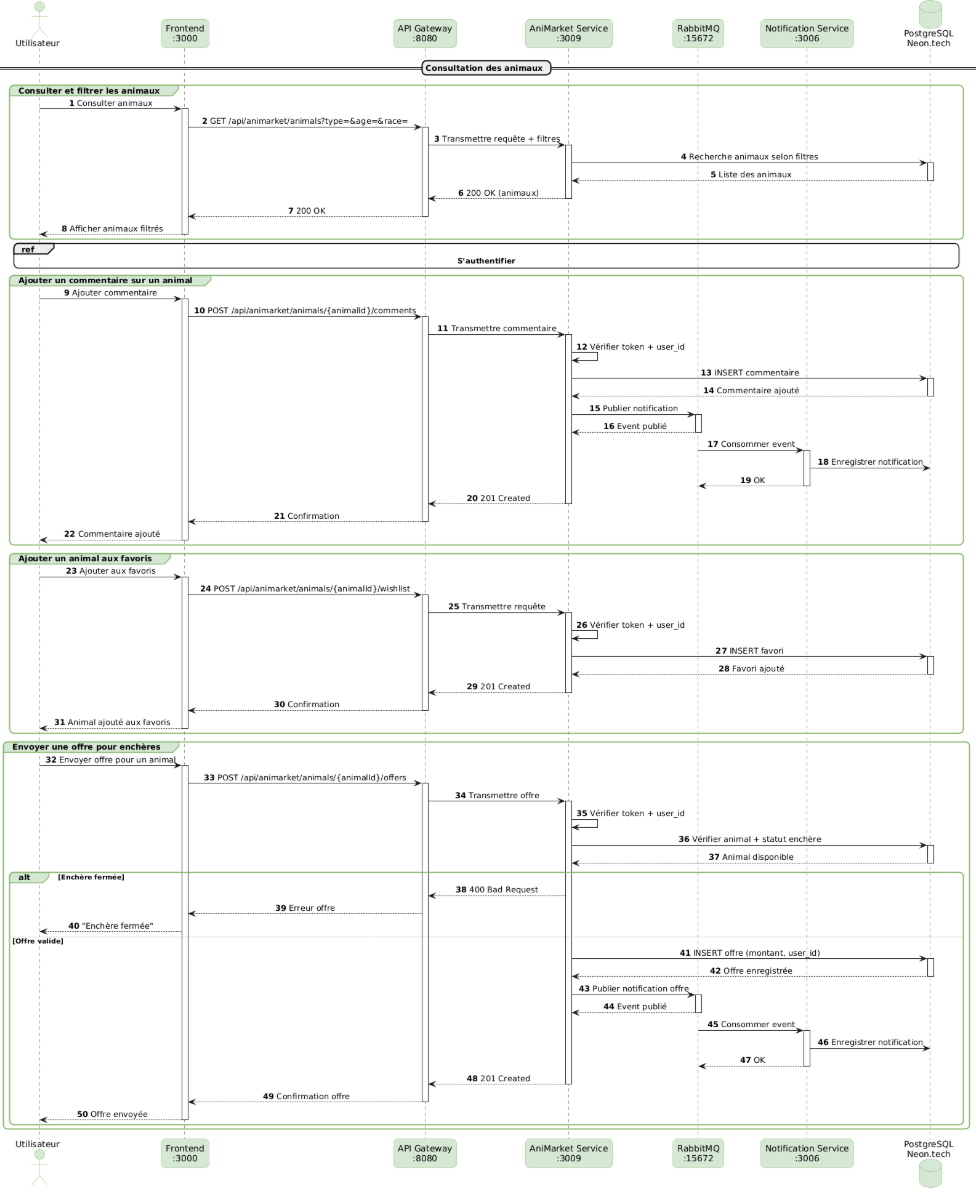
\includegraphics[width=0.75\textwidth]{images/consulter animaux animarket sq.png}
    \caption{Diagramme de séquence : consultation des animaux à vendre}
    \label{fig:animarket_consultation}
\end{figure} 
\newpage 
\subsubsection{Diagramme de séquence : gestion des animaux}

Cette figure illustre les interactions du vendeur avec le système pour la gestion de ses animaux, notamment l’ajout, la modification et la suppression : 

\begin{figure}[H]
    \centering
    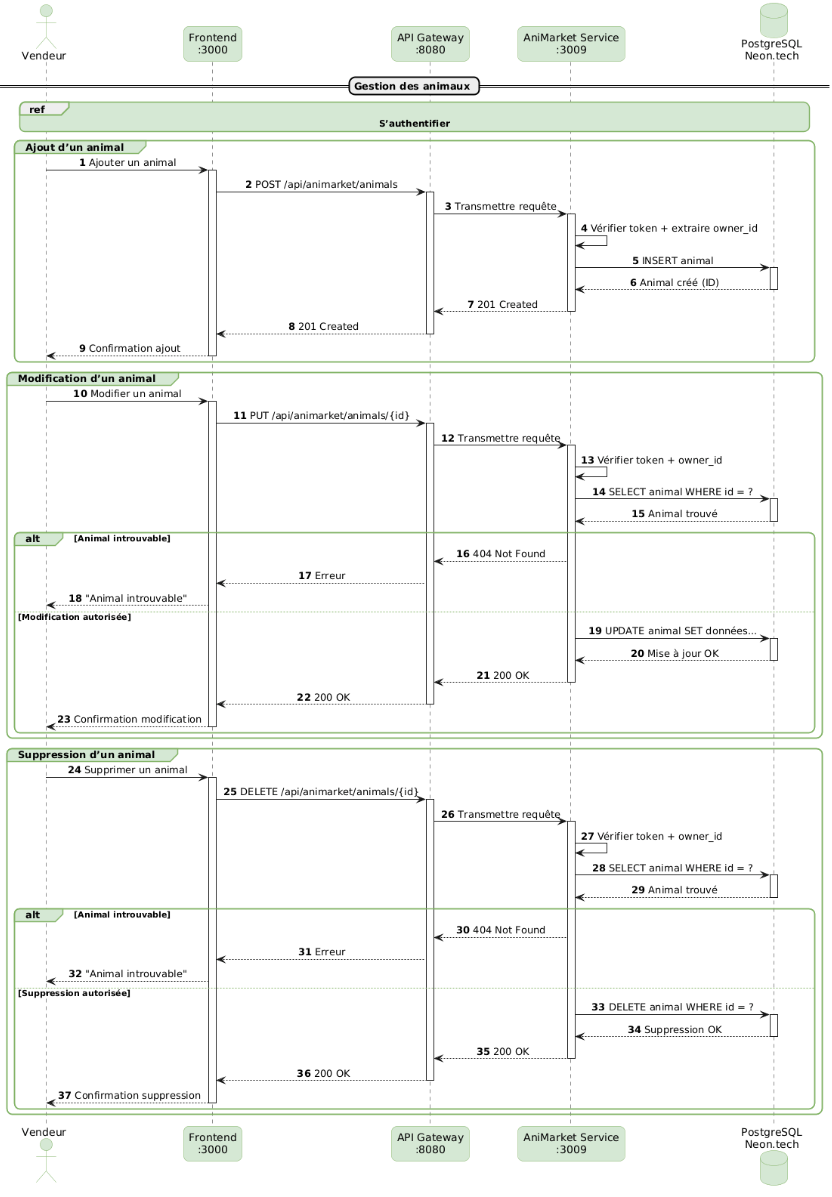
\includegraphics[width=0.78\textwidth]{images/gerer aimaux animarket sq.png}
    \caption{Diagramme de séquence : gestion des animaux}
    \label{fig:gestion_animaux}
\end{figure}





\newpage 
\subsection{Réalisation du sprint 4} 

\subsubsection{Menu principal de l’application AniHub et interface d’accueil AniMarket} 

Cette figure illustre le menu principal de l’application AniHub ainsi que l’interface d’accueil du module AniMarket : 

\begin{figure}[h!]
    \centering
    
    \begin{minipage}{0.48\textwidth}
        \centering
        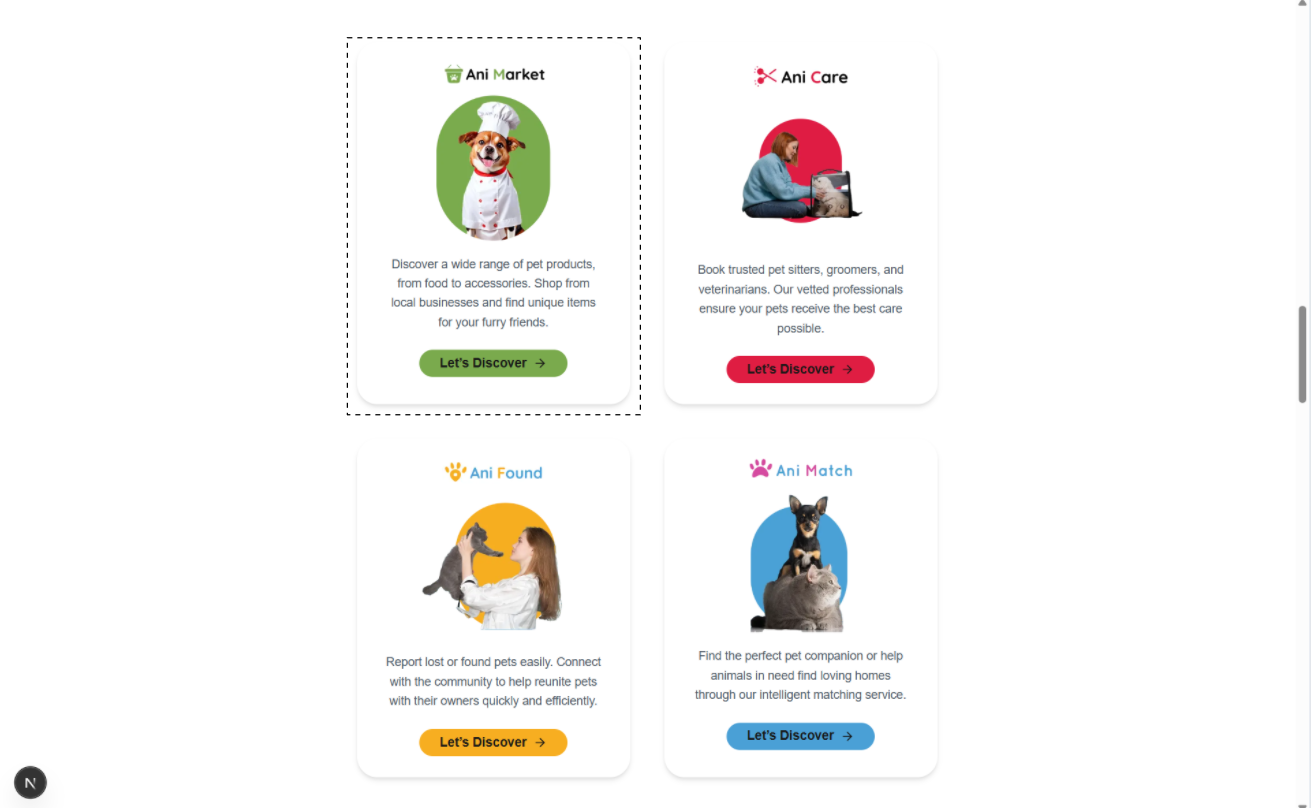
\includegraphics[width=0.85\textwidth]{images/menu animarket.png}
        \caption{Menu principal de l’application AniHub}
    \end{minipage}
    \hfill
    \begin{minipage}{0.48\textwidth}
        \centering
        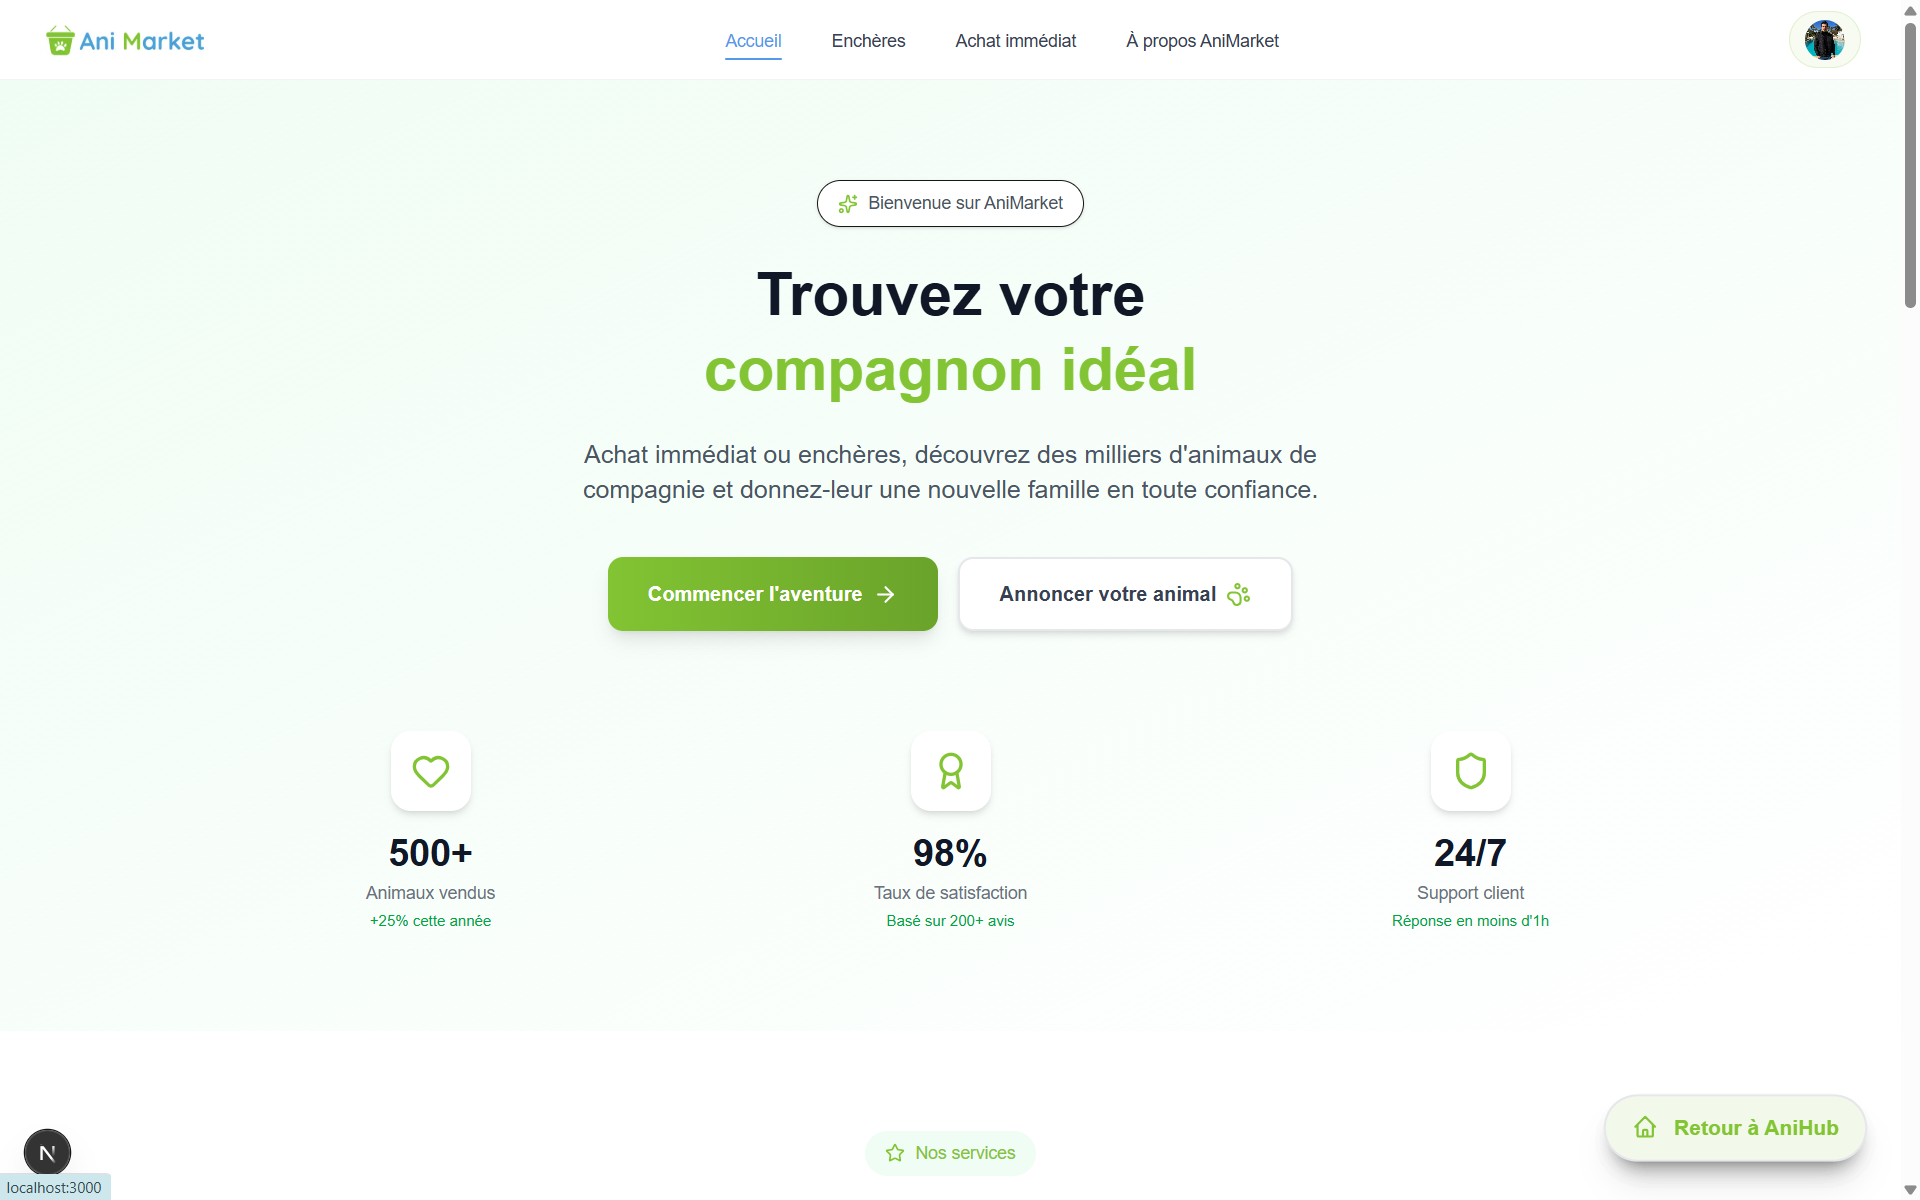
\includegraphics[width=0.85\textwidth]{images/home.png}
        \caption{Interface d’accueil AniMarket}
    \end{minipage}

\end{figure}   

\subsubsection{Interface d’annonce d’animal pour vente (enchère ou prix fixe)} 
La figure ci-dessous illustre l’interface d’annonce d’animal pour vente, où l’utilisateur peut choisir entre une enchère ou un prix fixe : 
\begin{figure}[h!]
    \centering
    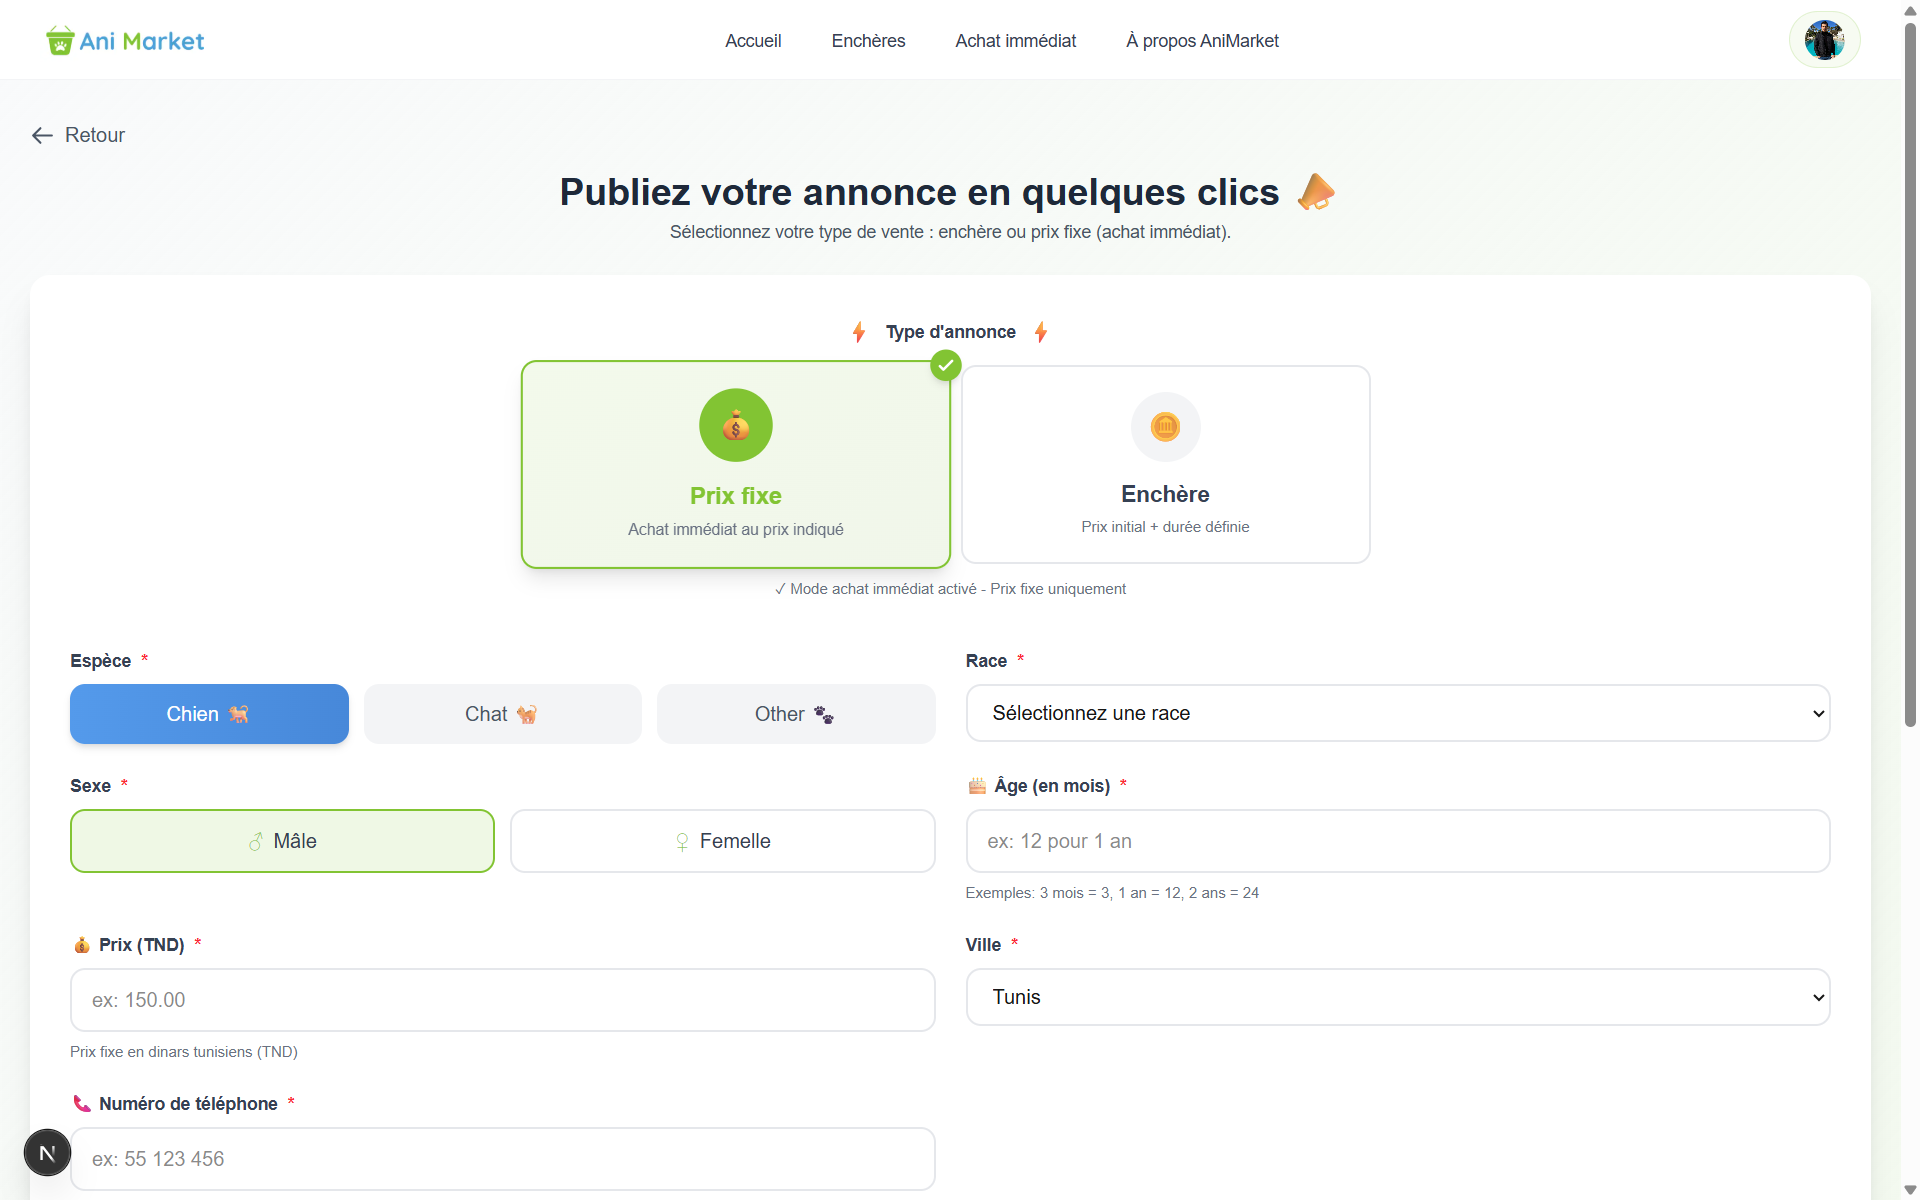
\includegraphics[width=0.77\textwidth]{images/annoncer animal.png}
    \caption{Interface d’annonce d’animal pour vente}
\end{figure}   

\newpage  
\subsubsection{Interface des achats immédiats (prix fixe)}

La figure ci-dessous illustre la page des achats immédiats (prix fixe) : 
\begin{figure}[h!]
    \centering
    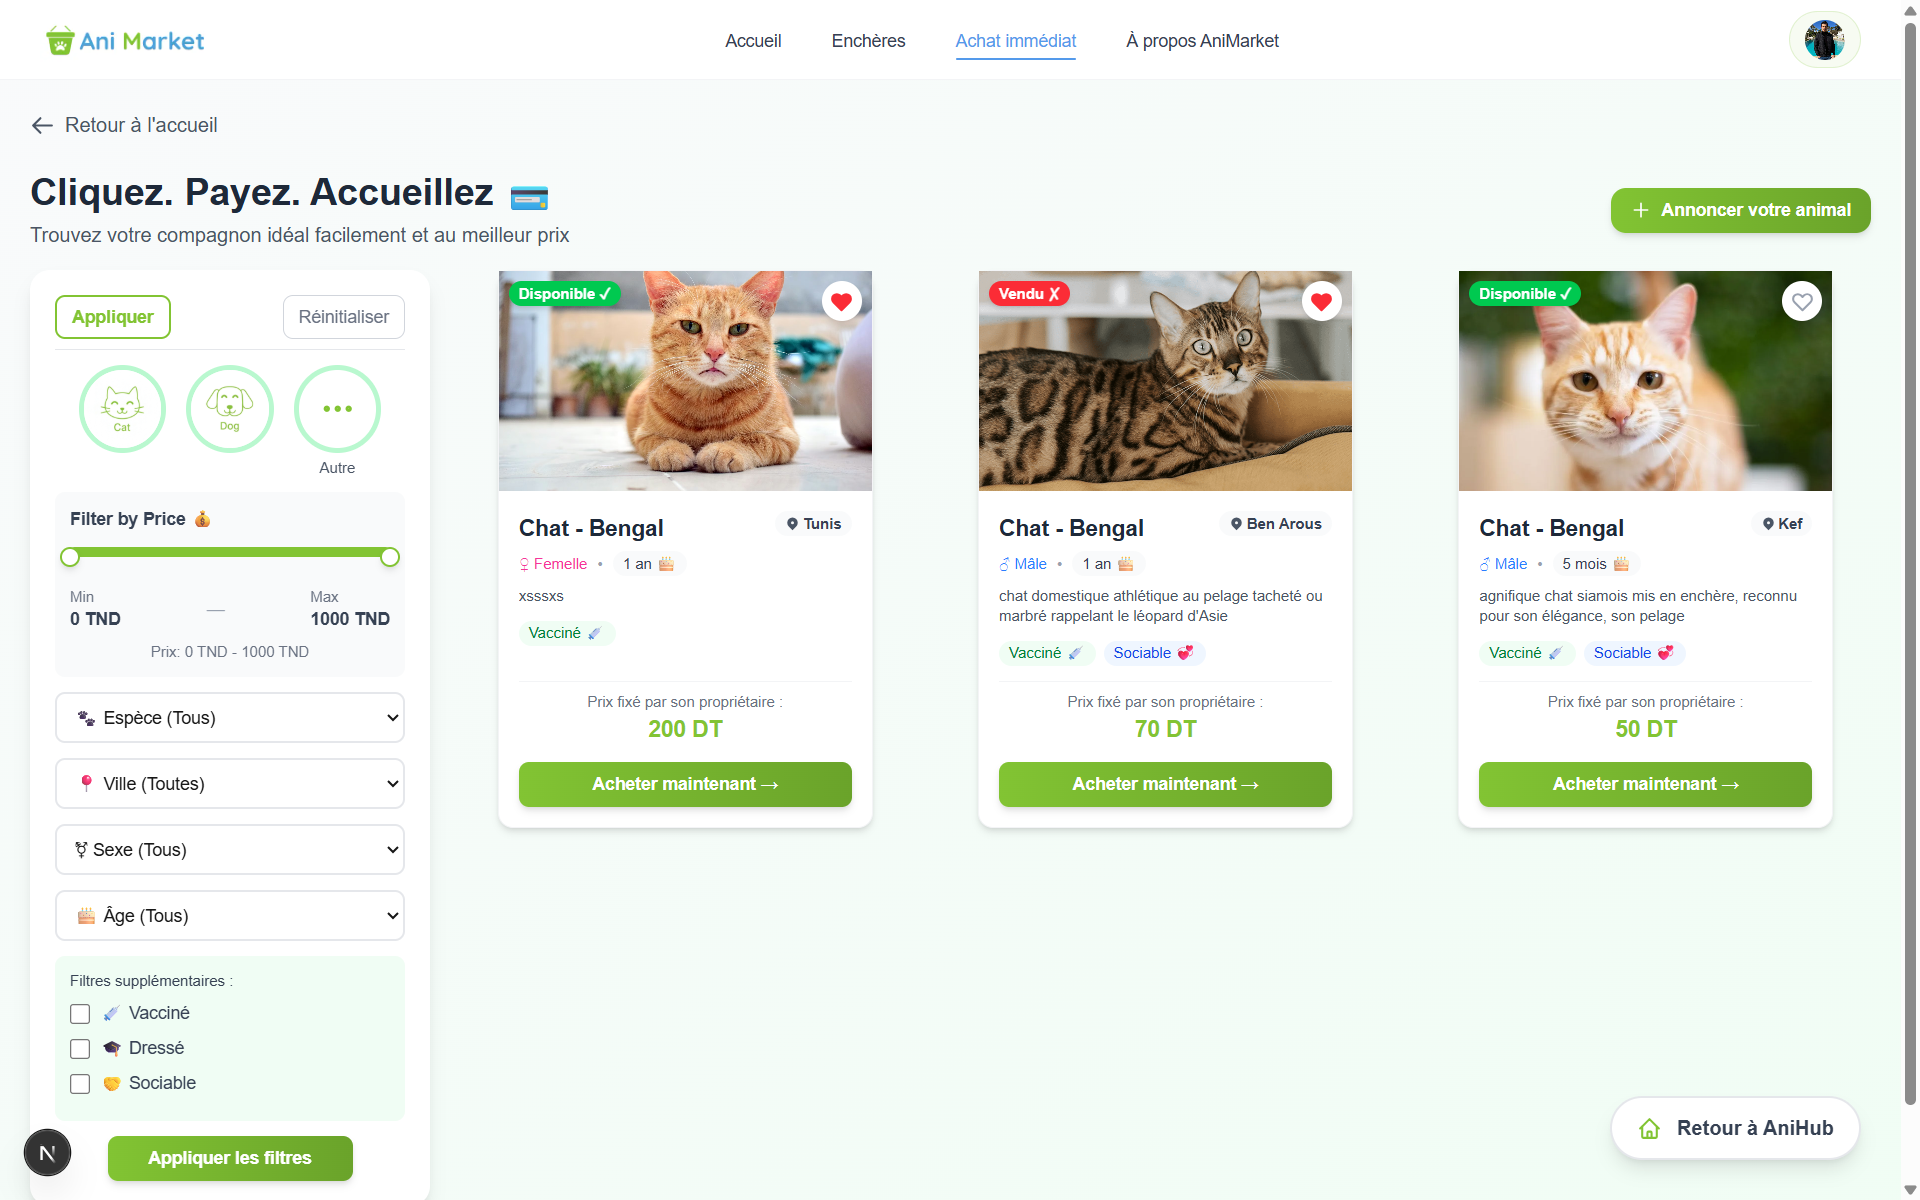
\includegraphics[width=0.77\textwidth]{images/page prix fixe.png}
    \caption{Interface des achats immédiats}
\end{figure}    


\subsubsection{Interface des enchères}

La figure ci-dessous illustre la page des enchères : 
\begin{figure}[h!]
    \centering
    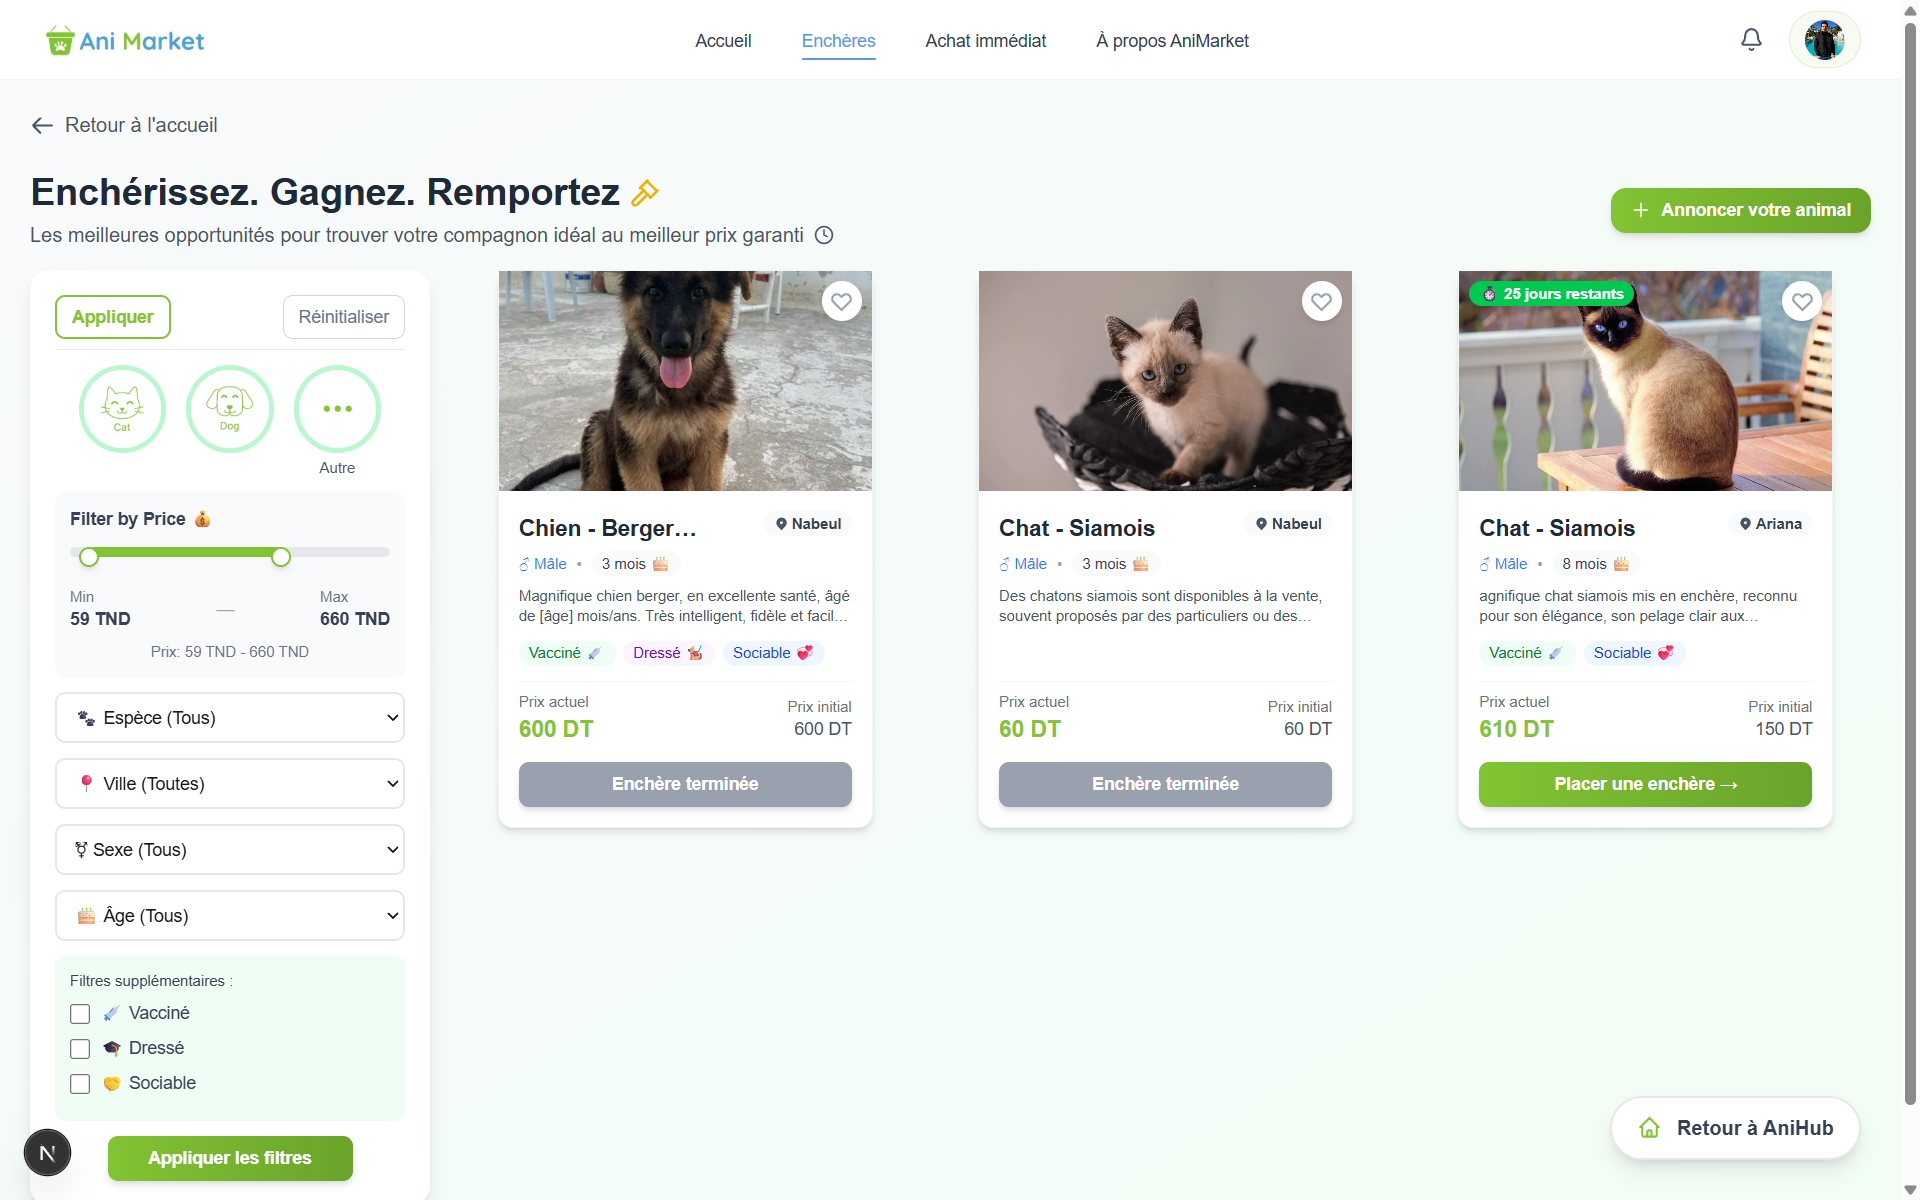
\includegraphics[width=0.77\textwidth]{images/page enchere.png}
    \caption{Interface des enchères}
\end{figure}    
\newpage 
\subsubsection{Interface détails d’une enchère et des offres}

La figure ci-dessous illustre l’interface de détails d’une enchère, présentant les offres proposées, le prix actuel ainsi qu’un formulaire permettant à l’utilisateur de soumettre sa propre offre : 

\begin{figure}[h!]
    \centering
    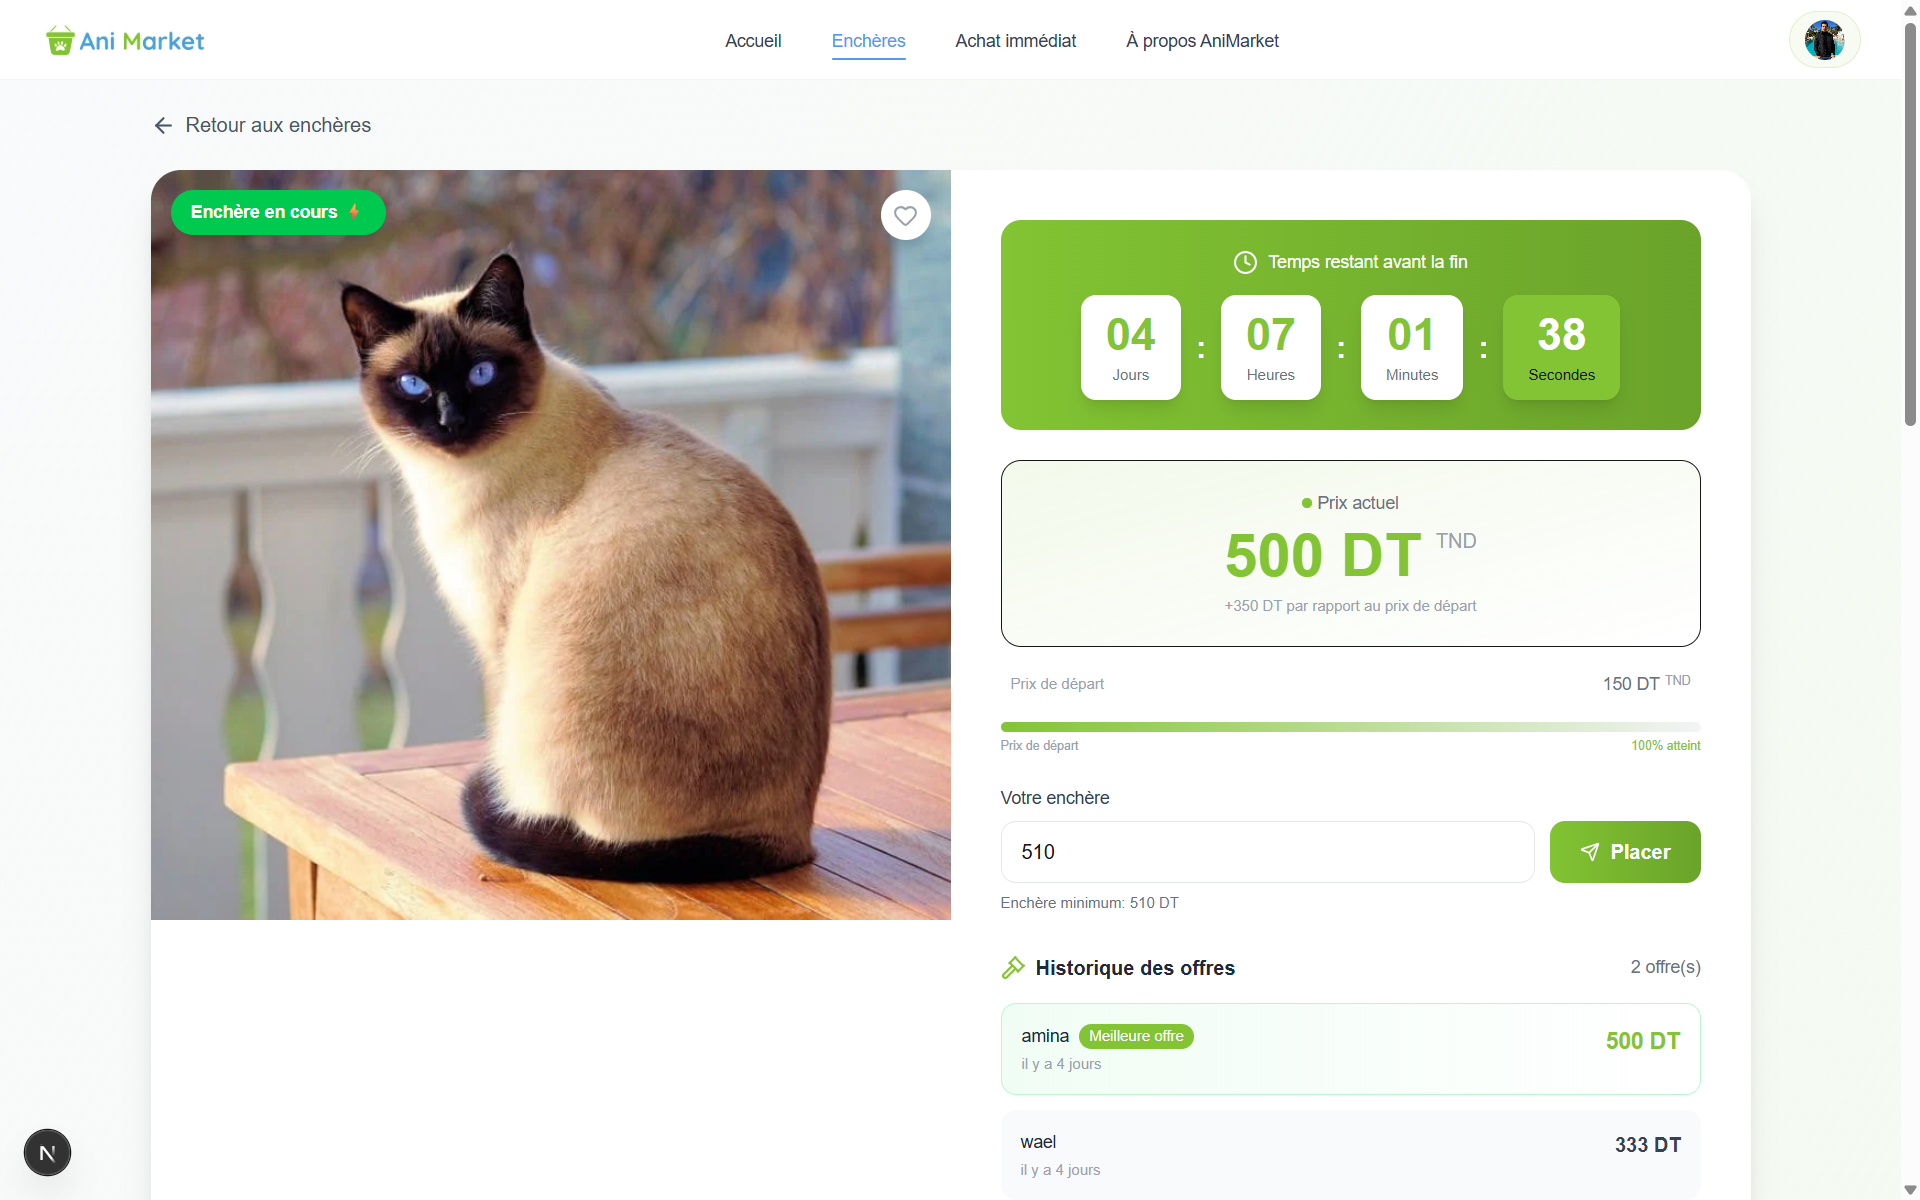
\includegraphics[width=0.75\textwidth]{images/details enchere.png}
    \caption{Interface détails d’une enchère}
\end{figure}    

\subsubsection{Interface des commentaires, avis et enchères similaires}

La figure ci-dessous illustre l’interface des commentaires, avis et enchères similaires : 

\begin{figure}[h!]
    \centering
    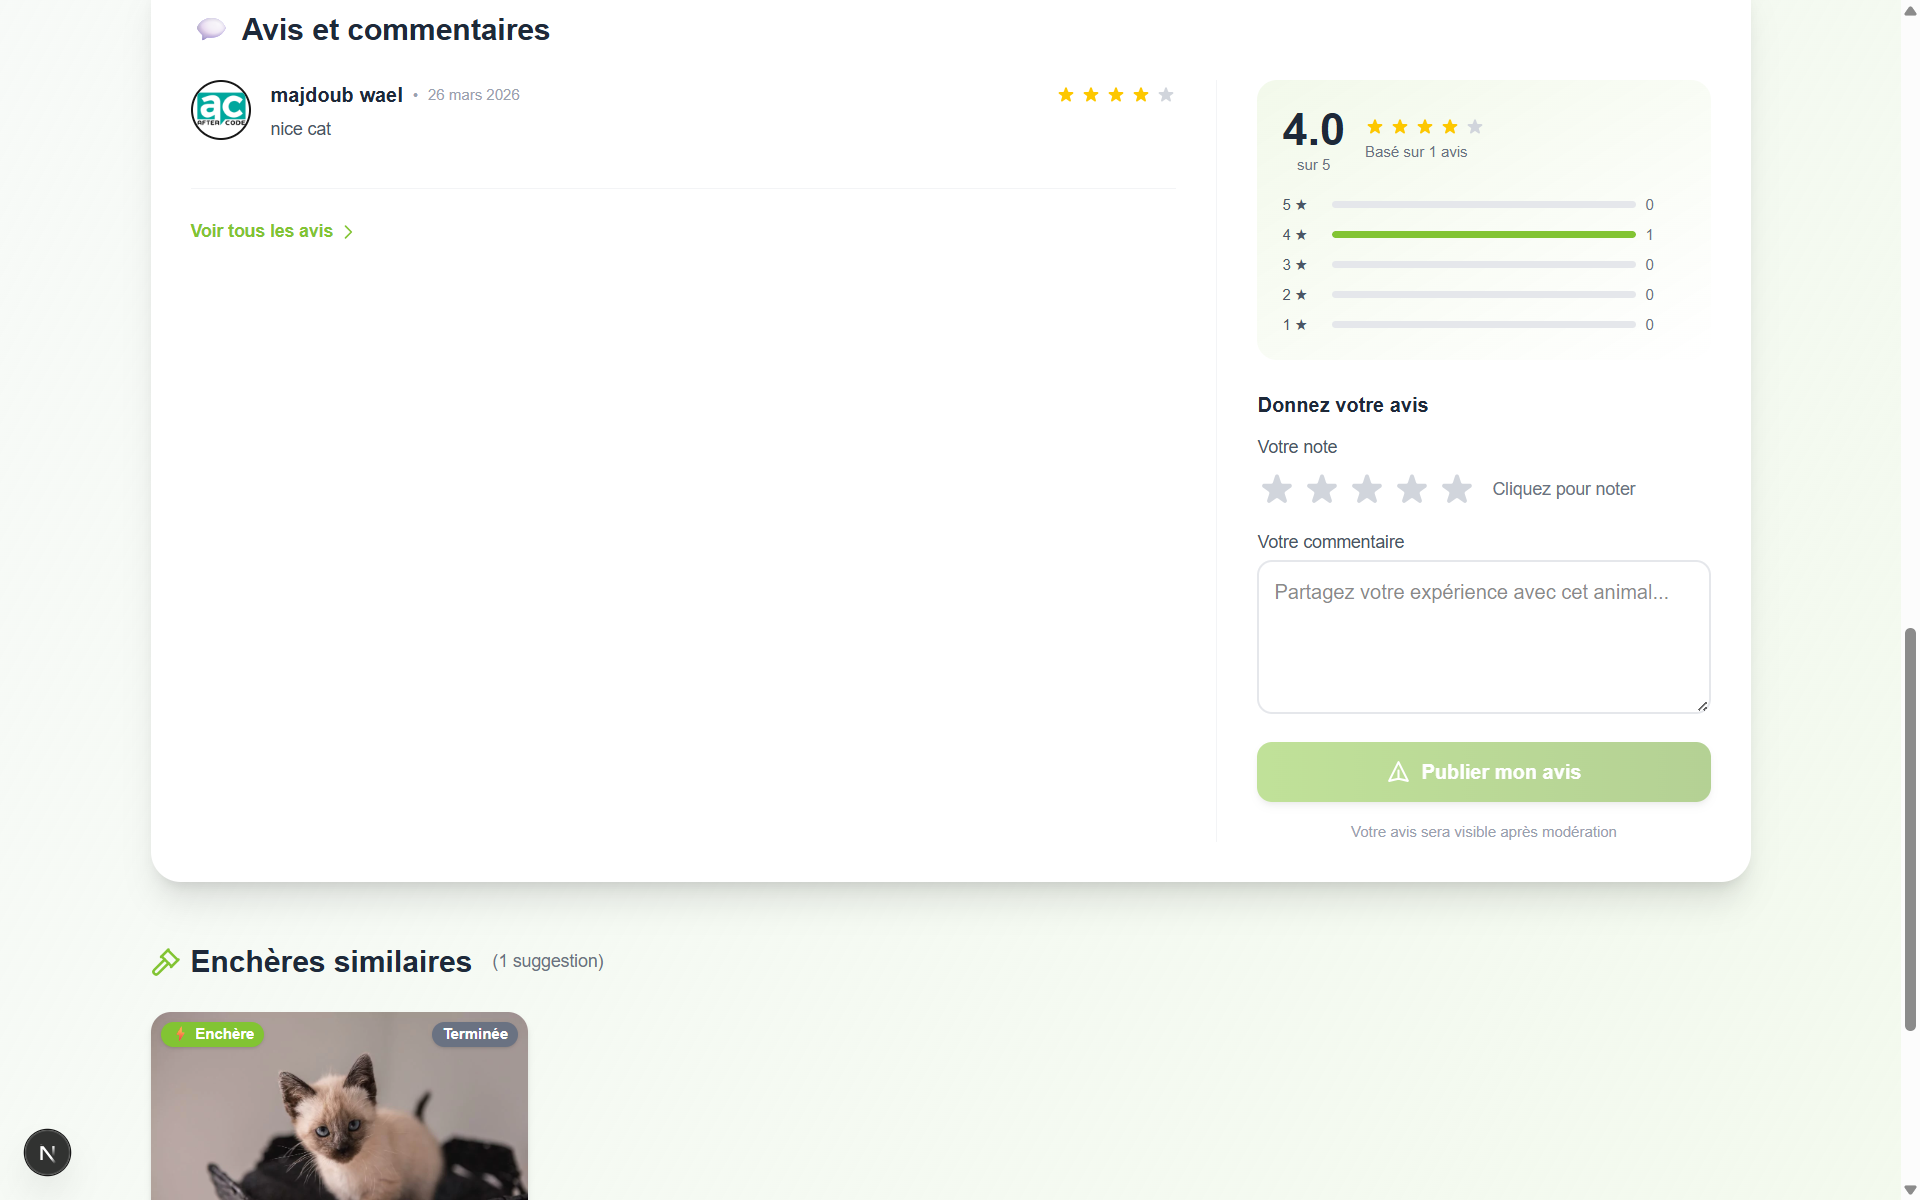
\includegraphics[width=0.72\textwidth]{images/comment section animaux similaires.png}
    \caption{Interface des commentaires, avis et enchères similaires}
\end{figure}    
\newpage  

\subsubsection{Interface notifications reçues}
La figure ci-dessous illustre les notifications reçues par un utilisateur concernant son enchère : 
\begin{figure}[h!]
    \centering
    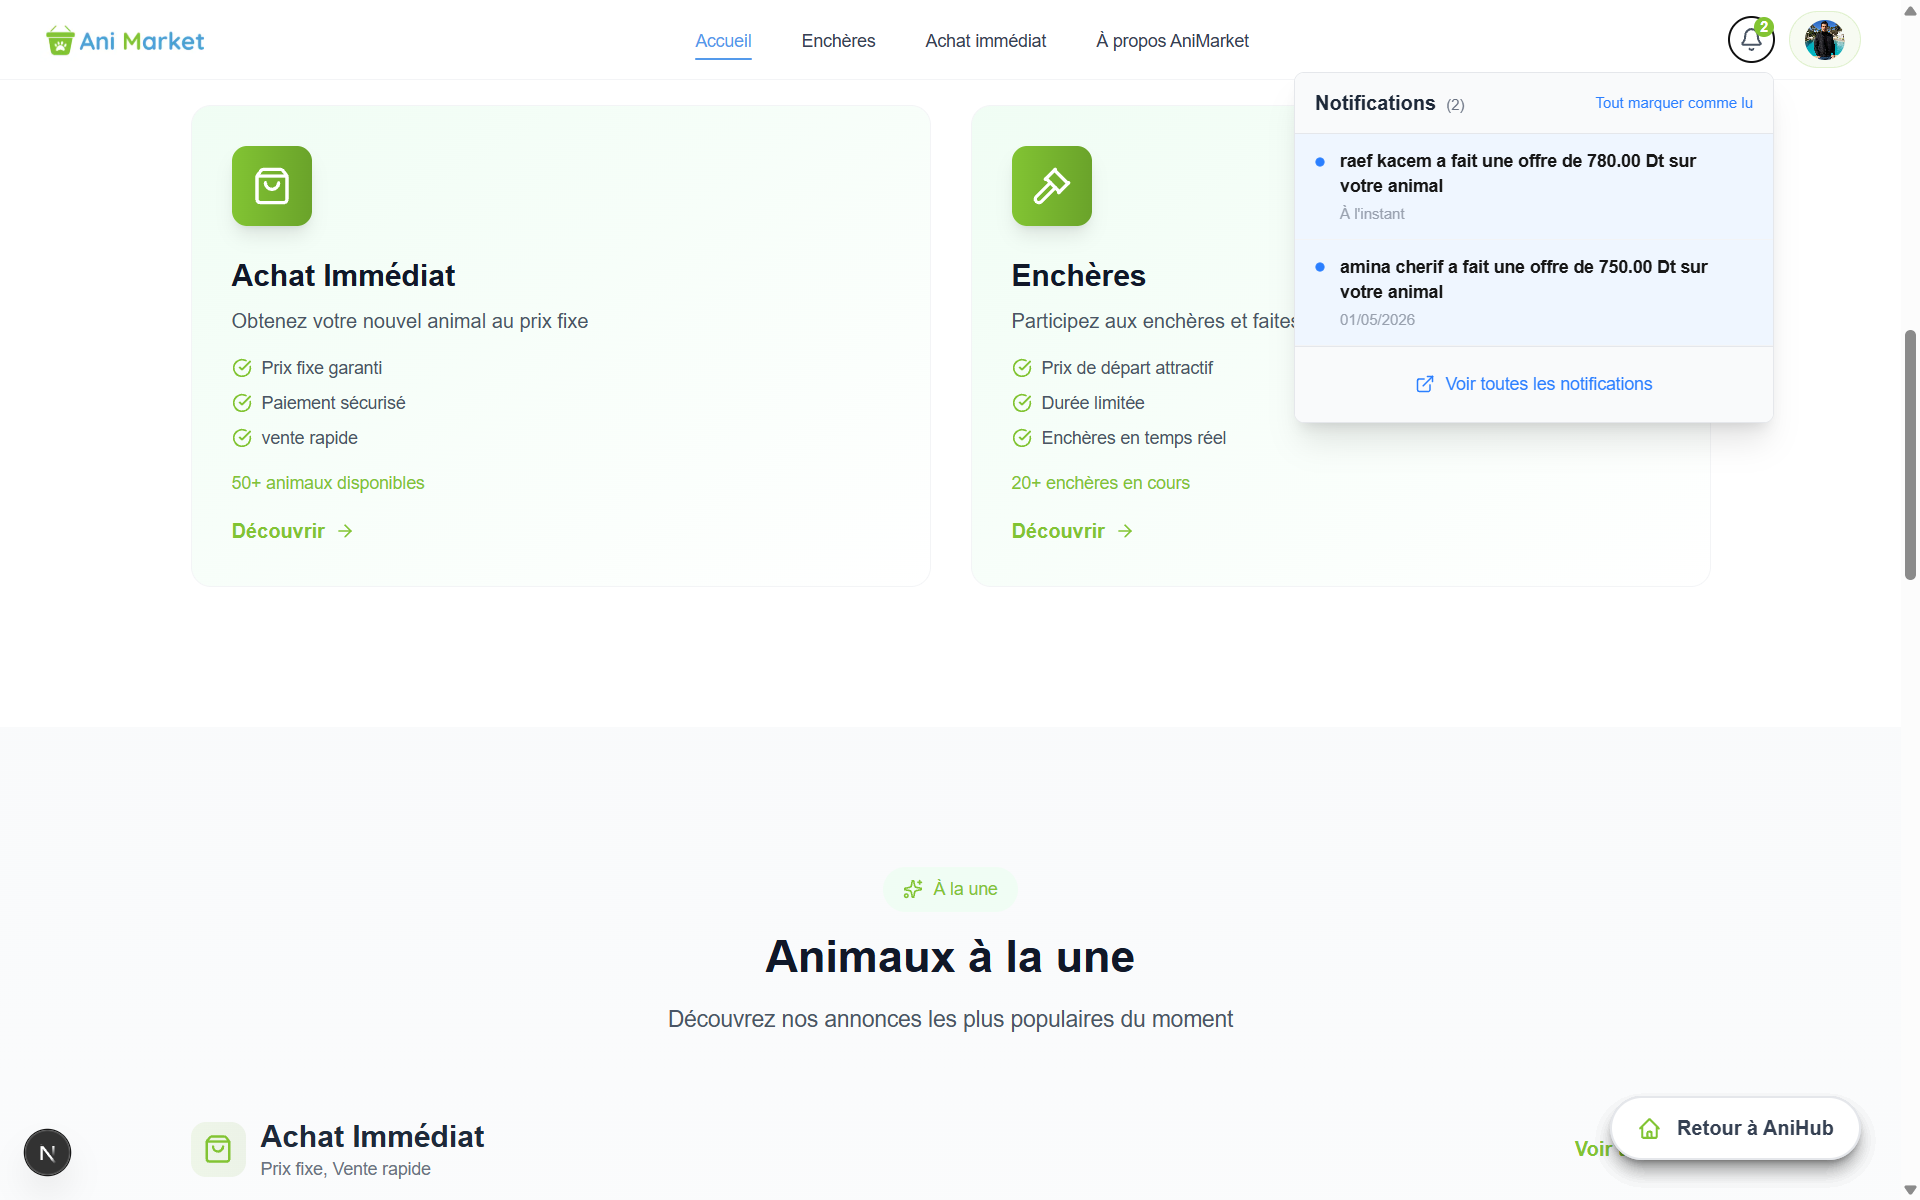
\includegraphics[width=0.77\textwidth]{images/notif animarket.png}
    \caption{Interface notifications reçues}
\end{figure}    

\subsubsection{Interface espace AniMarket} 
La figure ci-dessous présente l’interface AniMarket dédiée au vendeur : 
\begin{figure}[h!]
    \centering
    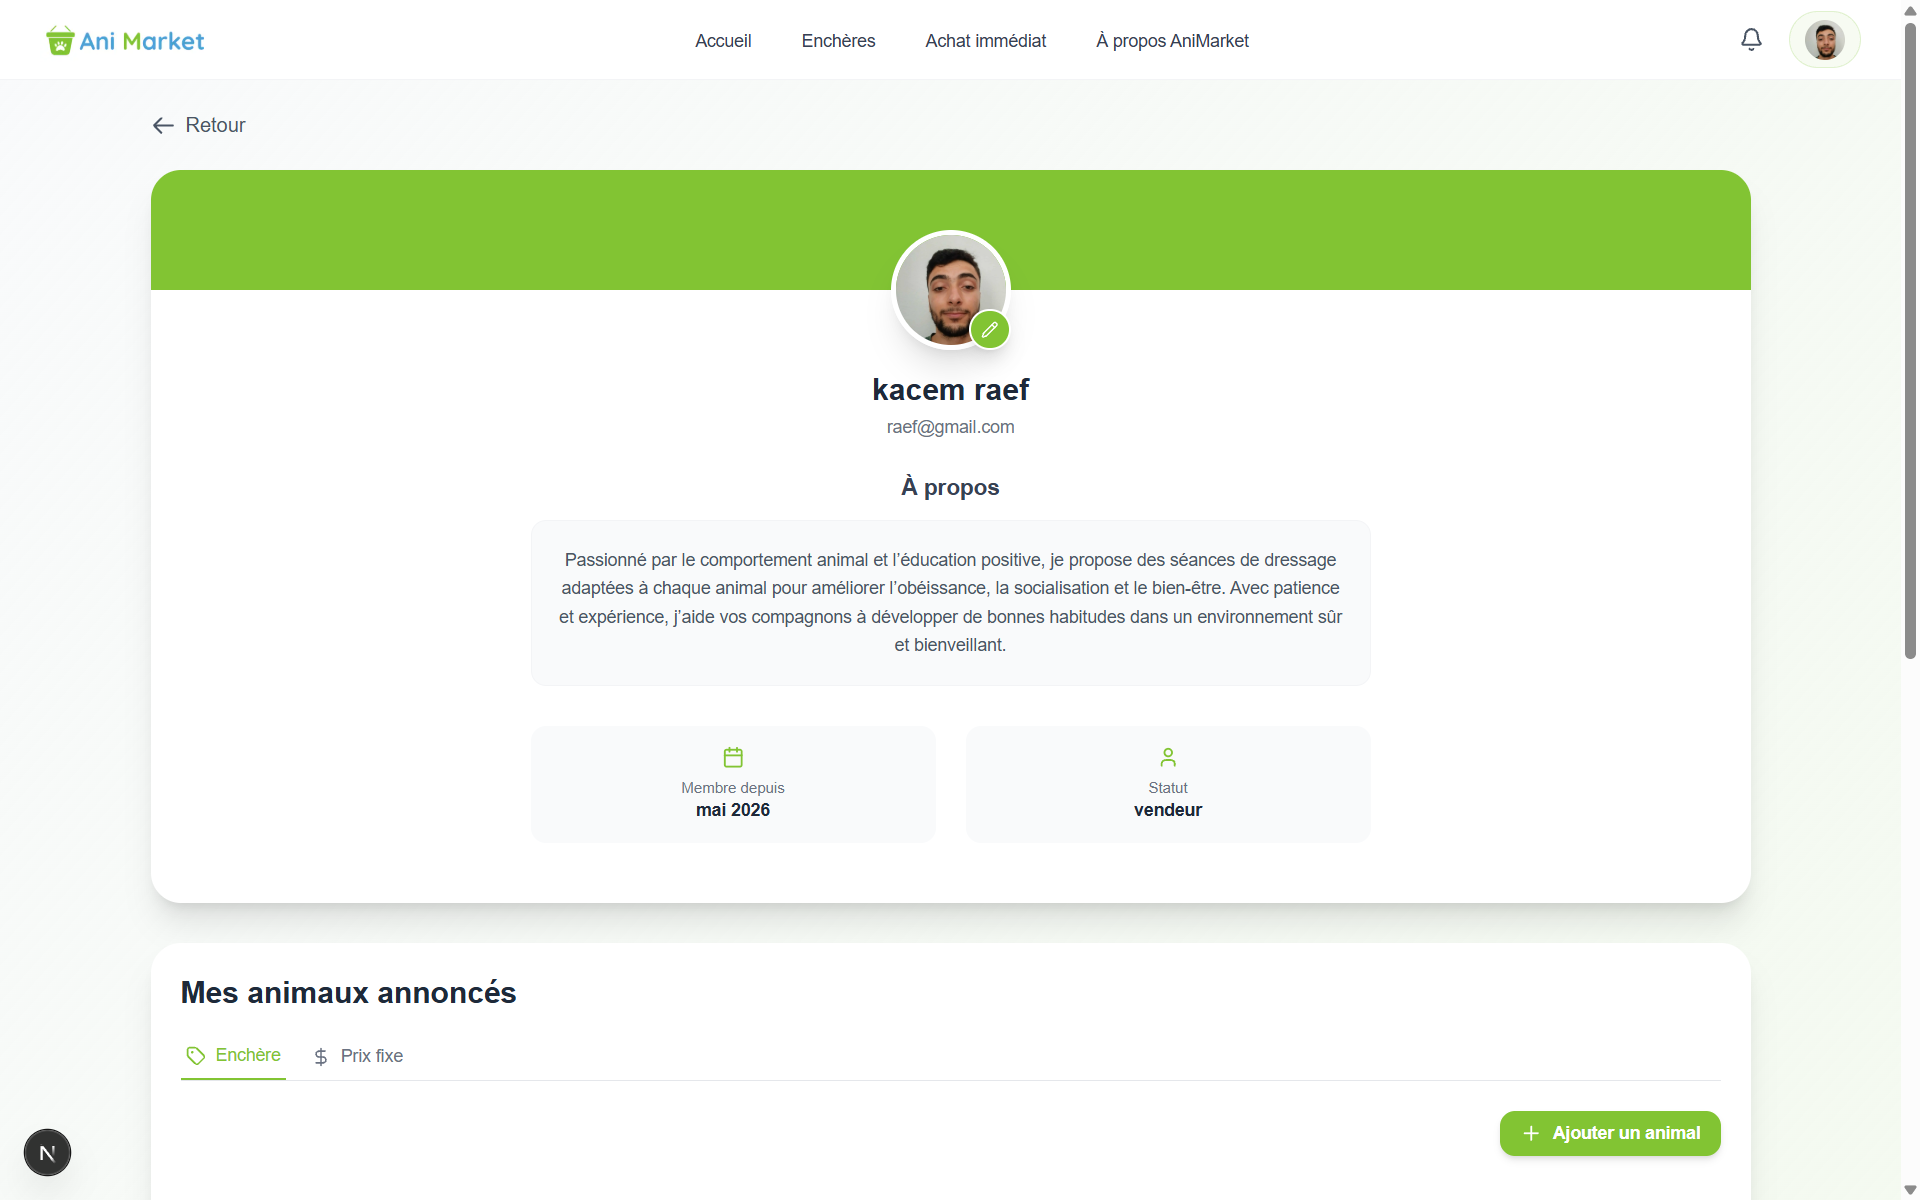
\includegraphics[width=0.77\textwidth]{images/espace animarket profil.png}
    \caption{Interface espace AniMarket}
\end{figure}  

\newpage 
\subsubsection{Interface mes animaux (prix fixe et enchère)} 
La figure ci-dessous illustre l’interface “Mes animaux” avec prix fixe et enchère : 
\begin{figure}[h!]
    \centering
    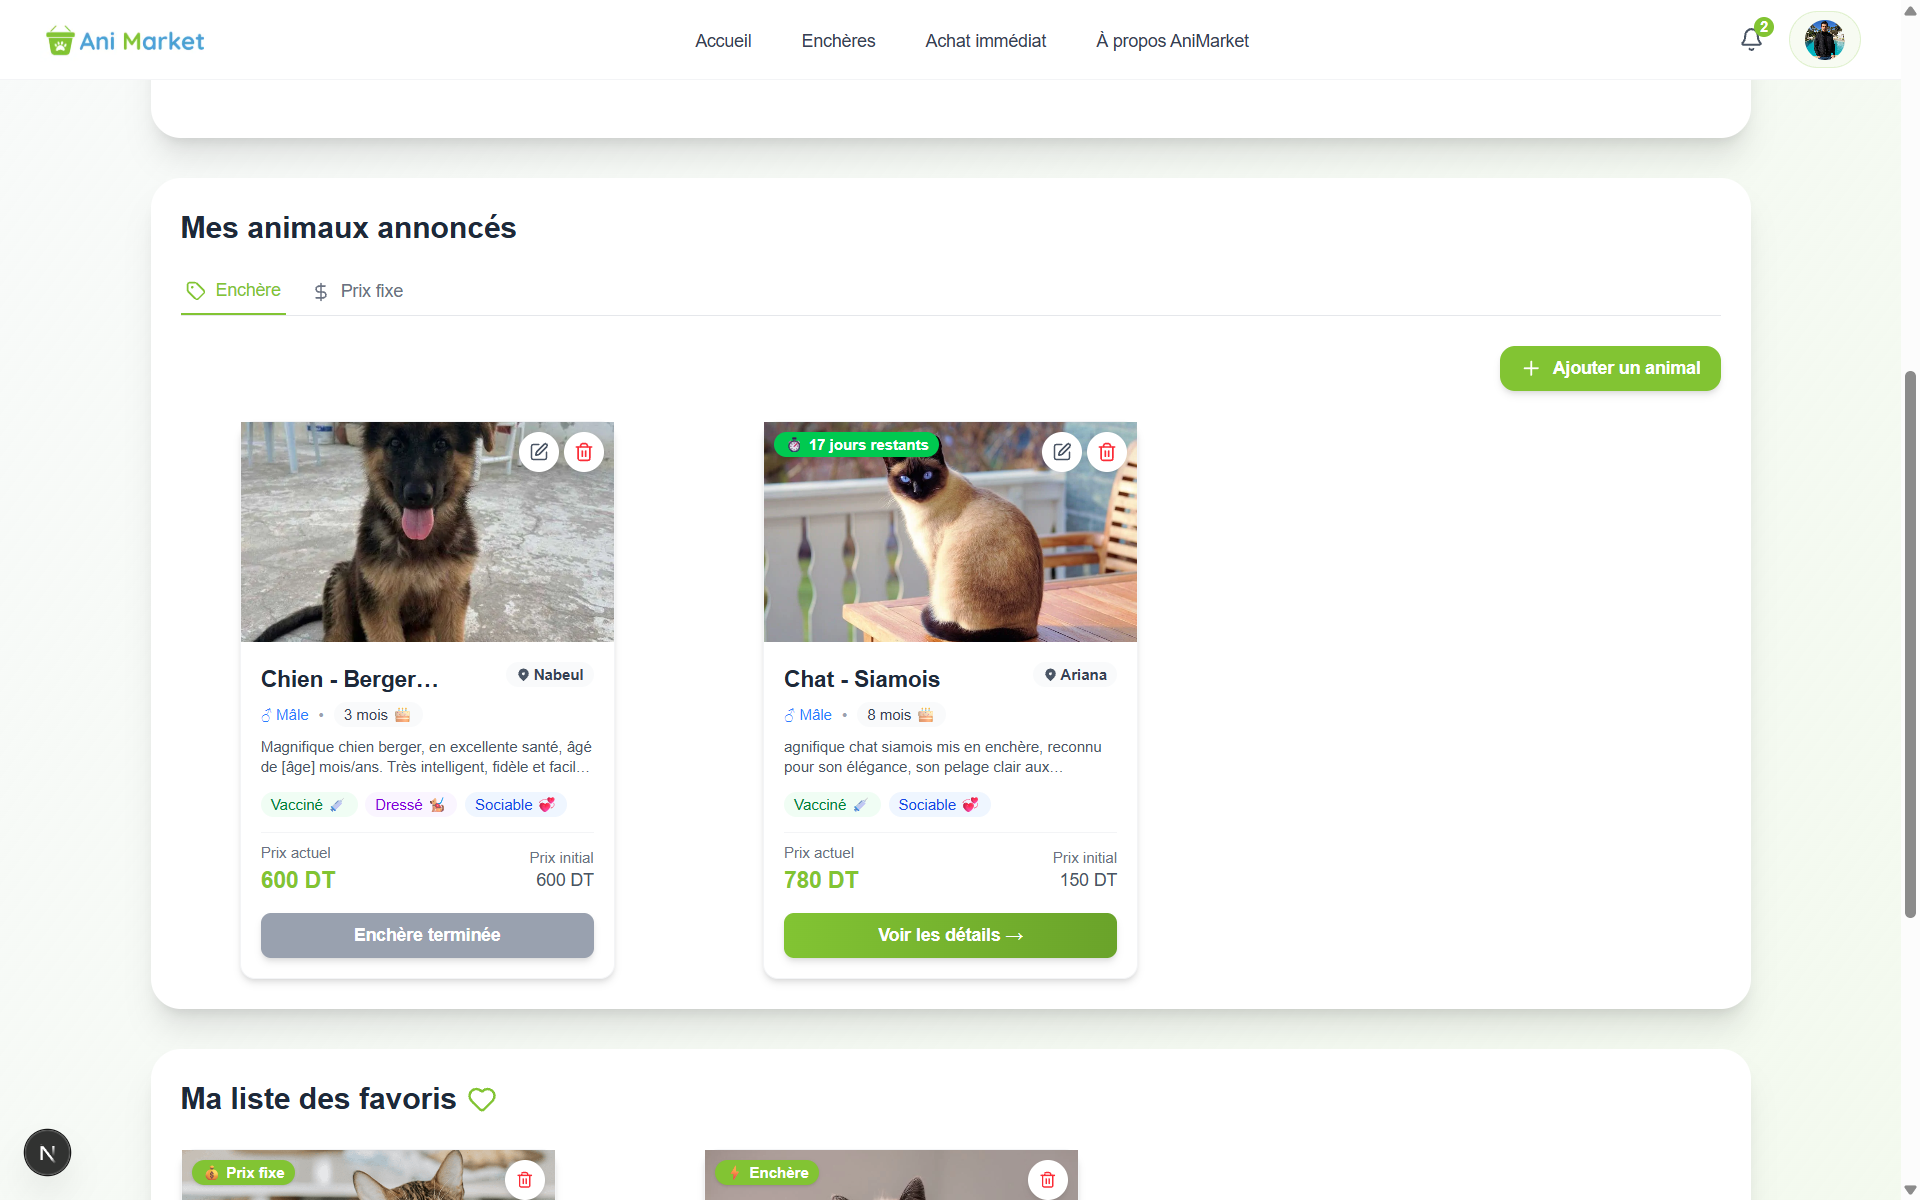
\includegraphics[width=0.77\textwidth]{images/mes animaux animarket.png}
    \caption{Interface mes animaux (prix fixe et enchère)}
\end{figure}  
\subsubsection{Interfaces modiifcation et suppression mes animaux}
Les figures ci-dessous présentent les interfaces de gestion des animaux (modification et suppression)

\begin{figure}[h!]
    \centering
    
    \begin{minipage}{0.48\textwidth}
        \centering
        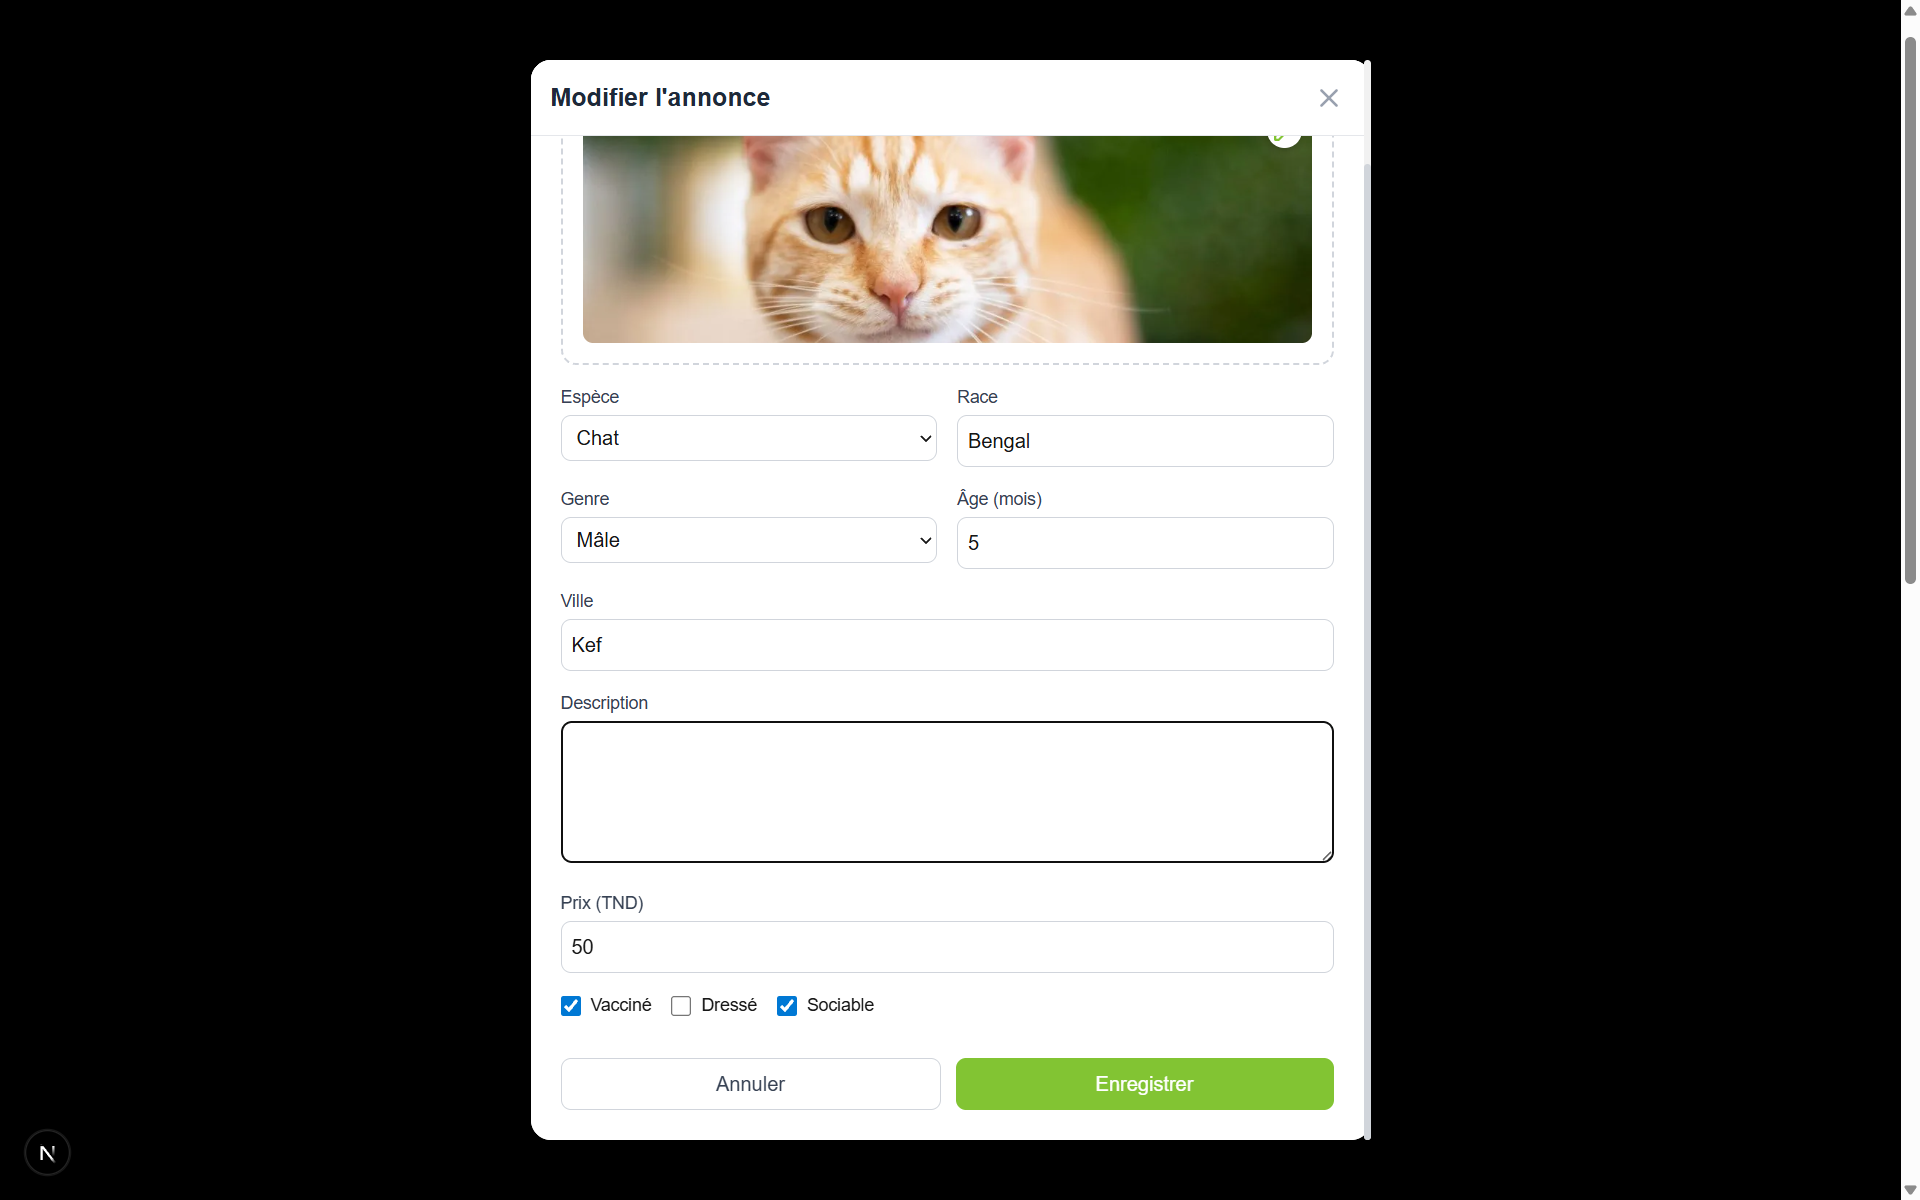
\includegraphics[width=0.85\textwidth]{images/modification animarket.png}
        \caption{Interface modification animal}
    \end{minipage}
    \hfill
    \begin{minipage}{0.48\textwidth}
        \centering
        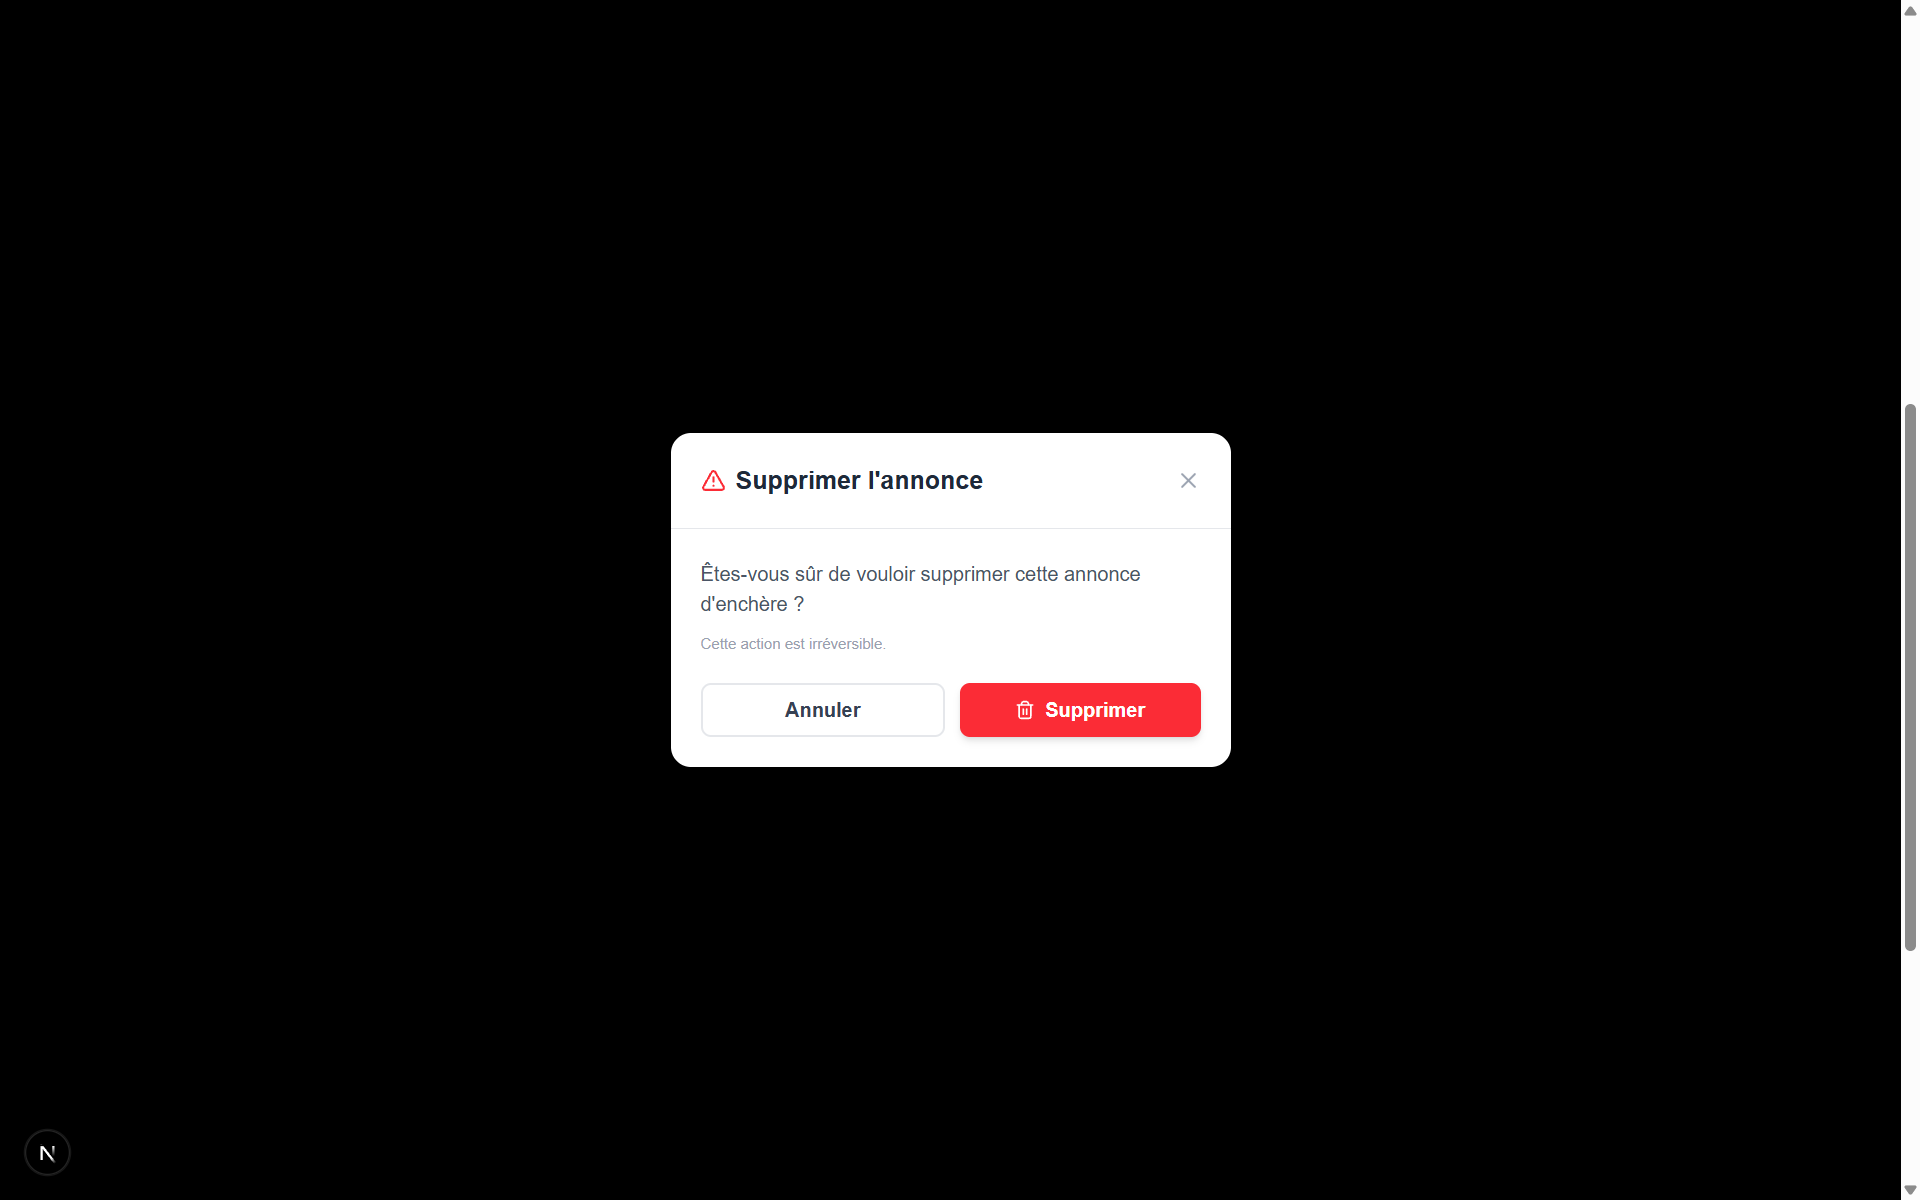
\includegraphics[width=0.85\textwidth]{images/suppression animarket.png}
        \caption{Interface suppression animal}
    \end{minipage}

\end{figure}   













\newpage 
\section{Sprint 5 : AniCare} 
\begin{figure}[H]
    \centering
    
\includegraphics[width=3.8cm]{images/logo anicare.png}
    \caption{Logo du module AniCare}
    \label{fig:logo-anicare}
\end{figure} 
Ce sprint, d’une durée de \textbf{3 semaines}, est dédié au module \textbf{AniCare}, qui permet la gestion et la mise en relation autour des services liés aux animaux. Il offre la possibilité de publier et consulter des services, de gérer les réservations, ainsi que de faciliter la communication entre les utilisateurs et les prestataires. 
\subsection{Sprint backlog}  
Le tableau suivant présente le Sprint Backlog du sprint 5 avec les user stories, les tâches associées et
les efforts estimés : 

\begin{longtable}{|p{2cm}|p{5cm}|p{6cm}|p{2cm}|}
\caption{Sprint Backlog du sprint 5}
\label{tab:sprint-anicare-backlog} \\ 
\hline
\rowcolor{coloranicare}
\textbf{ID} & \textbf{User Story} & \textbf{Tâches} & \textbf{Effort} \\
\hline
\endfirsthead

\hline
\rowcolor{coloranicare}
\textbf{ID} & \textbf{User Story} & \textbf{Tâches} & \textbf{Effort} \\
\hline
\endhead

% ===================== US1 =====================
\multirow{6}{2cm}{US1}
& \multirow{6}{5cm}{En tant qu’utilisateur, je veux consulter la liste des services afin de découvrir les services disponibles et choisir celui qui correspond le mieux à mes besoins}
& Conception UI (Figma) & 0.5 j \\
\cline{3-4}
& & API récupération des services & 1 j \\
\cline{3-4}
& & Filtrage et recherche des services & 0.5 j \\
\cline{3-4}
& & Pagination & 0.5 j \\
\cline{3-4}
& & Commenter et évaluer un service & 0.5 j \\ 
\cline{3-4}
& & ajouter aux favoris & 0.5 j \\
\cline{3-4} 
& & Consulter services similaires & 0.5 j \\
\cline{3-4} 
& & Intégration frontend/backend & 1 j \\
\cline{3-4}
& & Tests & 0.5 j \\
\hline

% ===================== US2 =====================
\multirow{7}{2cm}{US2}
& \multirow{7}{5cm}{En tant qu’utilisateur, je veux gérer mes réservations envoyées (envoyer, suivre, modifier, annuler) afin de gérer efficacement mes demandes}
& Conception UI (Figma) & 0.5 j \\
\cline{3-4}
& & APIs de création, de modification et d’annulation pour mes réservations & 1 j \\
\cline{3-4} 
& & Réserver un service & 0.5 j \\
\cline{3-4}
& & Consulter le statut de mes réservations (acceptée , en attente ou refusée) et modifier ou annuler & 0.5 j \\
\cline{3-4}
& & tests & 0.5 j \\
\hline

% ===================== US3 =====================
\multirow{5}{2cm}{US3}
& \multirow{5}{5cm}{En tant qu’utilisateur, je veux gérer mes notifications afin d’être informé des interactions sur mes activités}
& Analyse besoins notifications & 0.5 j \\
\cline{3-4}
& & Développement MS Notifications & 1 j \\
\cline{3-4}
& & Intégration RabbitMQ avec MS AniCare et le MS notifications & 0.5 j \\
\cline{3-4}
& & Création d’événements (réception, acceptation , refus etc.)& 0.5 j \\
\cline{3-4}
& & Interface notifications frontend & 0.5 j \\
\cline{3-4}
& & Marquer comme lu / non lu & 0.5 j \\
\hline

% ===================== US4 =====================
\multirow{5}{2cm}{US4}
& \multirow{5}{5cm}{En tant qu’utilisateur, je veux discuter avec l'autre partie (utilisateur ou prestataire)}
& Analyse & 0.5 j \\
\cline{3-4}
& & Intégration bouton WhatsApp & 0.5 j \\
\cline{3-4}
& & Génération lien wa.me & 0.5 j \\
\cline{3-4}
& & Tests & 0.5 j \\
\hline

% ===================== US5 =====================
\multirow{7}{2cm}{US5}
& \multirow{7}{5cm}{En tant que prestataire de service, je veux gérer mon propre service (publier, mettre à jour, supprimer) afin de présenter mes services de manière claire}
& Conception UI (Figma) & 0.5 j \\
\cline{3-4}
& & APIs création , modification et suppression service & 1 j \\
\cline{3-4} 
& & Intégration avec microservice Auth (JWT, sécurité API) & 0.5 j \\
\cline{3-4}
& & Upload d’images et de documents justificatifs sur Cloudinary& 0.5 j \\
\cline{3-4}
& & Intégration frontend/backend & 0.5 j \\ 
\cline{3-4} 
& & Tests & 0.5 j \\
\hline

% ===================== US6 =====================
\multirow{6}{2cm}{US6}
& \multirow{6}{5cm}{En tant que prestataire de service, je veux gérer mes réservations reçues afin de répondre aux demandes des clients et organiser efficacement mes prestations}
& Conception UI (Figma) & 0.5 j \\
\cline{3-4} 
& & APIs de récupération et de modification du statut (confirmée ou refusée) des réservations reçues & 1 j \\
\cline{3-4} 
& & Changement du statut de la réservation (accepter ou refuser) depuis le frontend & 0.5 j \\
\cline{3-4}
& & Développement du calendrier du prestataire & 1 j \\
\cline{3-4}
& & Affichage des réservations des utilisateurs dans le calendrier du prestatire & 0.5 j \\
\cline{3-4}
& & Tests & 0.5 j \\
\hline

\end{longtable}
\newpage 
\subsection{Diagramme des cas d’utilisation du sprint 5} 

Dans cette section, nous présentons le diagramme des cas d’utilisation du sprint 5, dédié au module \textbf{AniCare}. Ce diagramme illustre les principales interactions entre l’utilisateur et le prestataire de service avec le système . 

La figure ci-dessous représente le diagramme des cas d’utilisation correspondant : 


\begin{figure}[H]
    \centering
  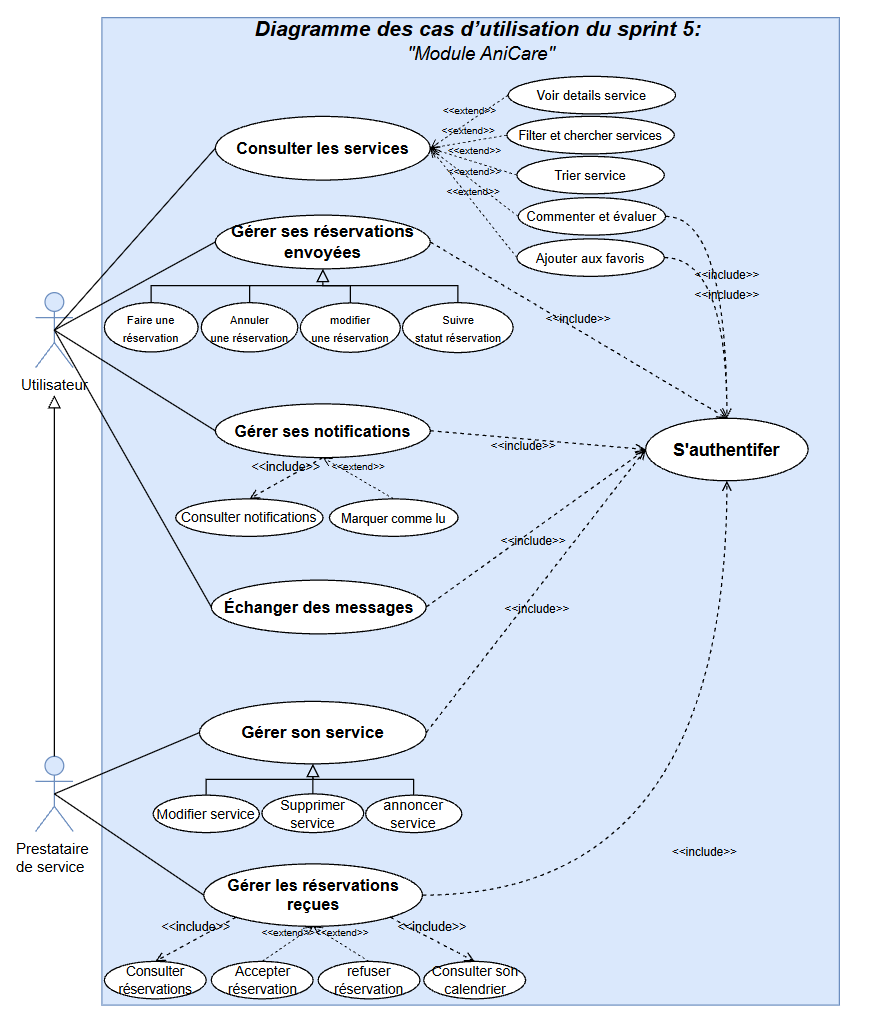
\includegraphics[width=1.05\linewidth, height=19.5cm, keepaspectratio]{images/use case anicare.png}
    \caption{Diagramme des cas d’utilisation du sprint 5}
    \label{fig:usecase-sprint5}
\end{figure} 

\newpage 
\subsection{Descriptions textuelles des cas d’utilisation du sprint 5}   
Cette section présente les cas d’utilisation du sprint 5 du module AniCare : 
\subsubsection{ Description textuelle du cas d’utilisation «Consulter les services» } 
Le tableau ci-dessous présente le cas d’utilisation « Consulter les services » :  

\begin{longtable}{|c|p{11cm}|}
\caption{Description textuelle du cas d’utilisation "Consulter les services"}
\label{tab:consulter_services} \\
\hline
\cellcolor{coloranicare} \textbf{Nom du cas d'utilisation } & Consulter les services \\
\hline
\cellcolor{coloranicare} \textbf{Acteurs} & Utilisateur \\
\hline
\cellcolor{coloranicare} \textbf{Description } & Tout utilisateur du système peut consulter les services du module "AniCare" proposés par les prestataires de service. \\
\hline
\cellcolor{coloranicare} \textbf{Pré-condition } & Accès libre à la page d’accueil sans authentification. \\
\hline
\cellcolor{coloranicare} \textbf{Post-condition } & L’utilisateur a consulté les services et peut interagir avec un service. \\
\hline

\cellcolor{coloranicare} \textbf{Scénario nominal } & 
\begin{enumerate}
\item L’utilisateur accède à la page d’accueil d’AniHub.
\item L’utilisateur choisit le module AniCare.
\item Le système redirige l’utilisateur vers AniCare.
\item L’utilisateur accède à la section « Services ».
\item Le système affiche la liste des services disponibles.
\item L’utilisateur peut filtrer les services selon des critères (type service , ville , etc.).
\item Le système affiche la liste des services filtrés.
\item L’utilisateur clique sur un service.
\item Le système affiche les détails du service.
\item L’utilisateur authentifié ajoute un service à sa wishlist.
\item Le système ajoute le service à la wishlist.
\item L’utilisateur authentifié peut saisir un commentaire, attribuer une note et cliquer sur « Publier ».
\item Le système vérifie, enregistre le commentaire et la note et met à jour la liste des avis affichés.
\end{enumerate} \\

\hline
\cellcolor{coloranicare} \textbf{Scénario alternatif :} &
Message d’erreur affiché si l’utilisateur n’est pas authentifié lors de l’ajout à la wishlist ou de la publication d’un commentaire. \\
\hline

\end{longtable}
 \newpage 
 \subsection{Description textuelle du cas d’utilisation «Gérer ses réservations envoyées»} 
\begin{longtable}{|c|p{11cm}|}
\caption{Description textuelle du cas d’utilisation "Gérer ses réservations envoyées"}
\label{tab:gerer_reservations_envoyees} \\
\hline
\cellcolor{coloranicare} \textbf{Nom du cas d'utilisation } & Gérer ses réservations envoyées \\
\hline
\cellcolor{coloranicare} \textbf{Acteurs} & Utilisateur \\
\hline
\cellcolor{coloranicare} \textbf{Description } & 
L’utilisateur peut envoyer une réservation, consulter  statut, modifier ou annuler une réservation existante. \\
\hline

\cellcolor{coloranicare} \textbf{Pré-condition } & L’utilisateur doit être authentifié. \\
\hline

\cellcolor{coloranicare} \textbf{Post-condition } & Les réservations envoyées sont traitées avec succès.\\
\hline

\cellcolor{coloranicare} \textbf{Scénario nominal } &
\begin{enumerate}
\item L’utilisateur accède à « AniCare » et choisit la section « Services ».
\item Le système affiche la liste des services disponibles.
\item L’utilisateur clique sur un service.
\item Le système affiche les détails du service.

\item Selon l’action de l’utilisateur :

\begin{itemize}

\item \textbf{Cas 1 : Envoi d’une réservation}
\begin{enumerate}
\item L’utilisateur choisit un créneau et envoie une réservation.
\item Le système enregistre la réservation.
\item Le système notifie le prestataire.
\end{enumerate}

\end{itemize}

\item L’utilisateur accède à « Mon espace AniCare ».
\item Le système affiche la liste des réservations envoyées.
\item L’utilisateur sélectionne une réservation.

\begin{itemize}

\item \textbf{Cas 2 : Modification d’une réservation}
\begin{enumerate}
\item L’utilisateur modifie les informations et valide.
\item Le système met à jour la réservation.
\end{enumerate}

\item \textbf{Cas 3 : Annulation d’une réservation}
\begin{enumerate}
\item L’utilisateur clique sur « Annuler ».
\item Le système supprime la réservation.
\end{enumerate}

\end{itemize}

\end{enumerate} \\
\hline

\cellcolor{coloranicare} \textbf{Scénario alternatif :} &
\begin{itemize}
\item Message d’erreur si le créneau sélectionné n’est plus disponible.
\item Message d’erreur si la réservation ne peut pas être modifiée ou annulée.
\end{itemize} \\
\hline

\end{longtable} 
\newpage 
\subsection{Description textuelle du cas d’utilisation «Gérer ses réservations reçues»} 
\begin{longtable}{|c|p{11cm}|}
\caption{Description textuelle du cas d’utilisation "Gérer ses réservations reçues"}
\label{tab:gerer_reservations_recues} \\
\hline
\cellcolor{coloranicare} \textbf{Nom du cas d'utilisation } & Gérer ses réservations reçues \\
\hline
\cellcolor{coloranicare} \textbf{Acteurs} & Prestataire de service \\
\hline
\cellcolor{coloranicare} \textbf{Description } & 
Le prestataire de service peut consulter son calendrier, accepter ou refuser les réservations reçues. \\
\hline

\cellcolor{coloranicare} \textbf{Pré-condition } & Le prestataire doit être authentifié. \\
\hline

\cellcolor{coloranicare} \textbf{Post-condition } & Les réservations sont mises à jour avec succès. \\
\hline

\cellcolor{coloranicare} \textbf{Scénario nominal } &
\begin{enumerate}
\item Le prestataire accède à « AniCare ».
\item Le prestataire accède à son espace AniCare.
\item Le système affiche les réservations reçues.
\item Le prestataire consulte son calendrier.
\item Le système affiche les réservations dans le calendrier.

\item Selon l’action du prestataire :

\begin{itemize}

\item \textbf{Cas 1 : Acceptation d’une réservation}
\begin{enumerate}
\item Le prestataire sélectionne une réservation.
\item Le prestataire clique sur « Accepter ».
\item Le système met à jour le statut de la réservation.
\item Le système notifie l’utilisateur.
\end{enumerate}

\item \textbf{Cas 2 : Refus d’une réservation}
\begin{enumerate}
\item Le prestataire sélectionne une réservation.
\item Le prestataire clique sur « Refuser ».
\item Le système met à jour le statut de la réservation.
\item Le système notifie l’utilisateur.
\end{enumerate}

\end{itemize}

\end{enumerate} \\
\hline

\cellcolor{coloranicare} \textbf{Scénario alternatif :} &
\begin{itemize}
\item Si aucune réservation n’est reçue, le système affiche un message indiquant qu’aucune réservation n’est disponible.
\item Si le créneau demandé est déjà occupé, le système empêche l’acceptation de la réservation.
\end{itemize} \\
\hline

\end{longtable} 
\newpage 
\subsubsection{Description textuelle du cas d’utilisation « Gérer mon service »}
\begin{longtable}{|c|p{11cm}|}
\caption{Description textuelle du cas d'utilisation "Gérer mon service"}
\label{tab:gerer_service} \\
\hline
\cellcolor{coloranicare}\textbf{Nom du cas d'utilisation } & Gérer mon service \\
\hline
\cellcolor{coloranicare}\textbf{Acteurs} & Prestataire de service \\
\hline
\cellcolor{coloranicare}\textbf{Description } & Le prestataire de service peut publier, modifier et supprimer ses services dans AniCare. \\
\hline
\cellcolor{coloranicare}\textbf{Pré-condition } & Le prestataire de service doit être authentifié. \\
\hline
\cellcolor{coloranicare}\textbf{Post-condition } & Les services sont correctement publiés, mis à jour ou supprimés. \\
\hline

\cellcolor{coloranicare}\textbf{Scénario nominal } &
\begin{enumerate}
\item L’utilisateur se connecte à son compte.
\item L’utilisateur sélectionne le module AniCare.
\item Le système redirige l’utilisateur vers AniCare.
\item L’utilisateur accède à son <<espace AniCare>>.
\item Le système affiche la liste de ses services.

\item \textbf{Cas publication :}
\begin{itemize}
\item L’utilisateur clique sur « Publier un service ».
\item Le système affiche un formulaire de création.
\item L’utilisateur saisit les informations du service et valide la publication.
\item Le système enregistre le service et l’affiche.
\end{itemize}

\item \textbf{Cas modification :}
\begin{itemize}
\item L’utilisateur sélectionne un service et clique sur « Modifier ».
\item Le système affiche le formulaire pré-rempli.
\item L’utilisateur modifie les informations du service.
\item Le système met à jour le service.
\end{itemize}

\item \textbf{Cas suppression :}
\begin{itemize}
\item L’utilisateur clique sur « Supprimer ».
\item Le système demande confirmation.
\item L’utilisateur confirme la suppression.
\item Le système supprime le service.
\end{itemize}

\item Le système affiche un message de succès.
\end{enumerate} \\
\hline

\cellcolor{coloranicare}\textbf{Scénario alternatif :} &
\begin{itemize}
\item En cas d’erreur lors de la publication ou de la modification, le système affiche un message d’erreur.
\item En cas d’annulation : le service est conservé.
\end{itemize} \\
\hline

\end{longtable}
\newpage 
\subsection{Diagramme des classes du sprint 5}   
La figure ci-dessous représente le diagramme de classes du sprint 5 dédié au module AniCare, illustrant les principales entités du système ainsi que leurs relations pour assurer le bon fonctionnement du module : 
\begin{figure}[H]
    \centering
    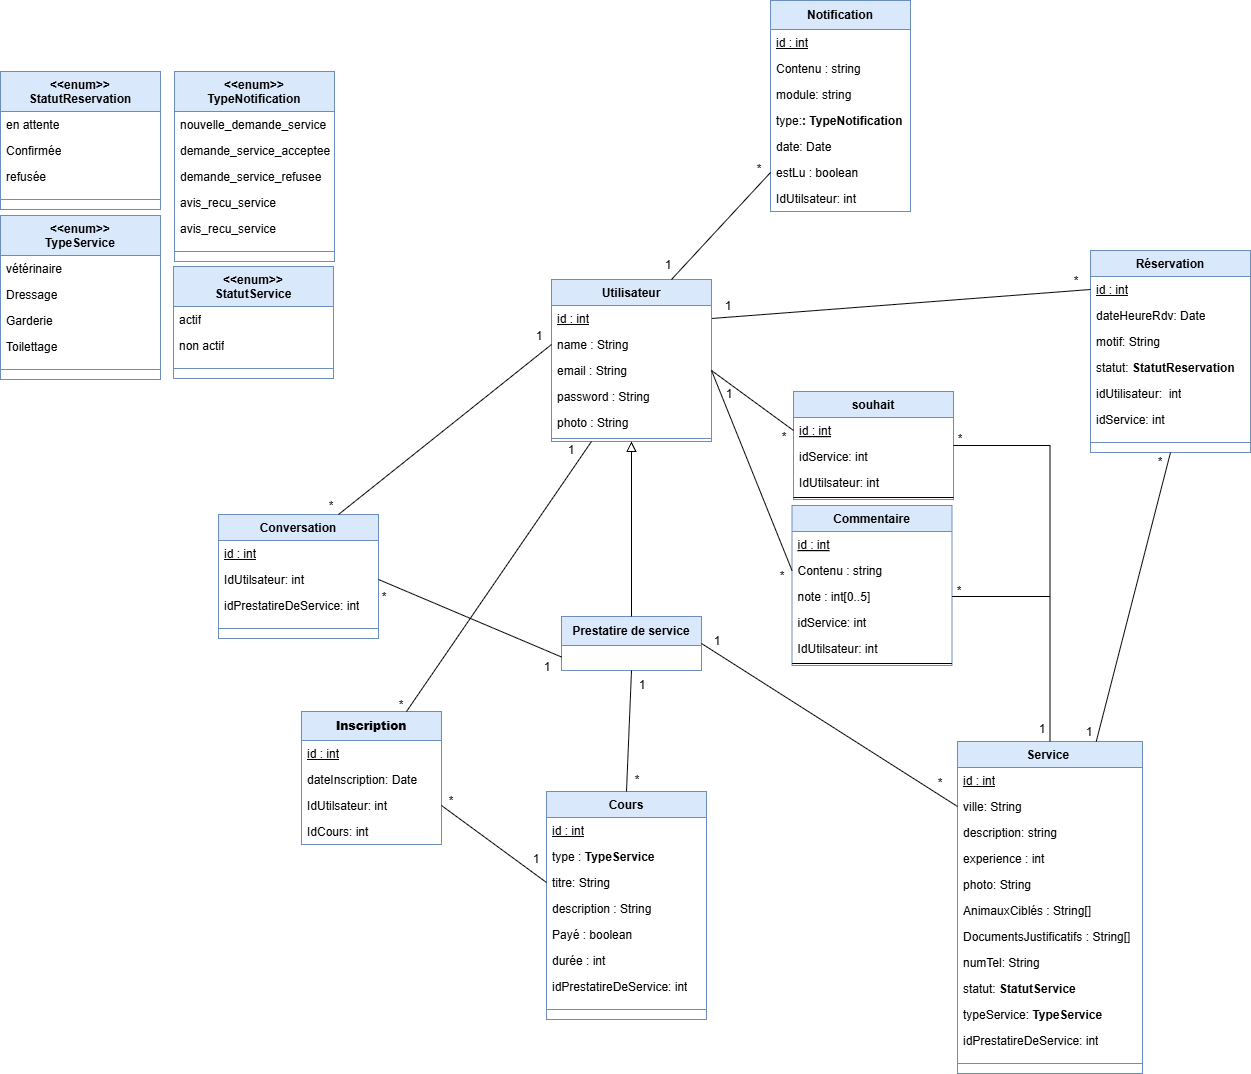
\includegraphics[width=18cm, height=20cm, keepaspectratio]{images/class digram anicare.png}
    \caption{Diagramme de classes de la sprint 5}
    \label{fig:class_diagram_sprint5}
\end{figure} 

\subsection{Diagrammes de séquence du sprint 5}

Cette section présente les diagrammes de séquence du cinquième sprint, qui illustrent les interactions entre les différents composants du système .  
\newpage 
\subsubsection{Diagramme de séquence : consultation  des services}

Cette figure illustre les interactions de l’utilisateur avec les services : consultation et filtrage (sans authentification), ainsi que les actions authentifiées comme les commentaires, les favoris (wishlist) et la réservation. Elle présente les échanges entre le frontend, l’API Gateway, le service AniCare, la base de données et le système de notification : 
\begin{figure}[H]
    \centering
    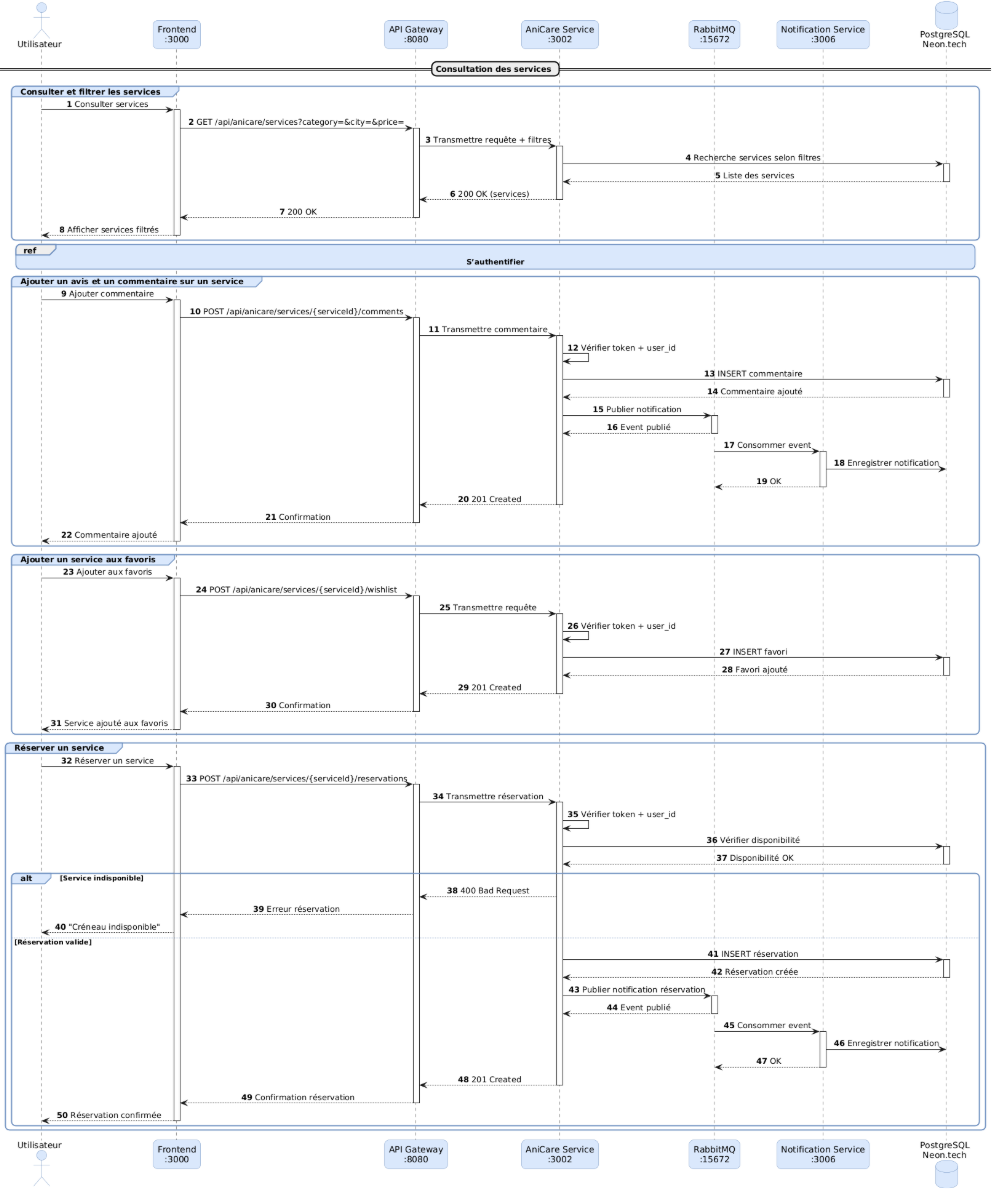
\includegraphics[width=0.85\textwidth]{images/consulter services sq.png}
    \caption{Diagramme de séquence : consultation  des services}
    \label{fig:services_utilisateur}
\end{figure}
\newpage 
\subsubsection{Diagramme de séquence : gestion des services}

Cette figure illustre les interactions du prestataire de service avec le système pour la gestion de ses services, notamment la création, la modification et la suppression. Elle met en évidence les échanges entre le frontend, l’API Gateway, le service AniCare et la base de données : 
\begin{figure}[H]
    \centering
    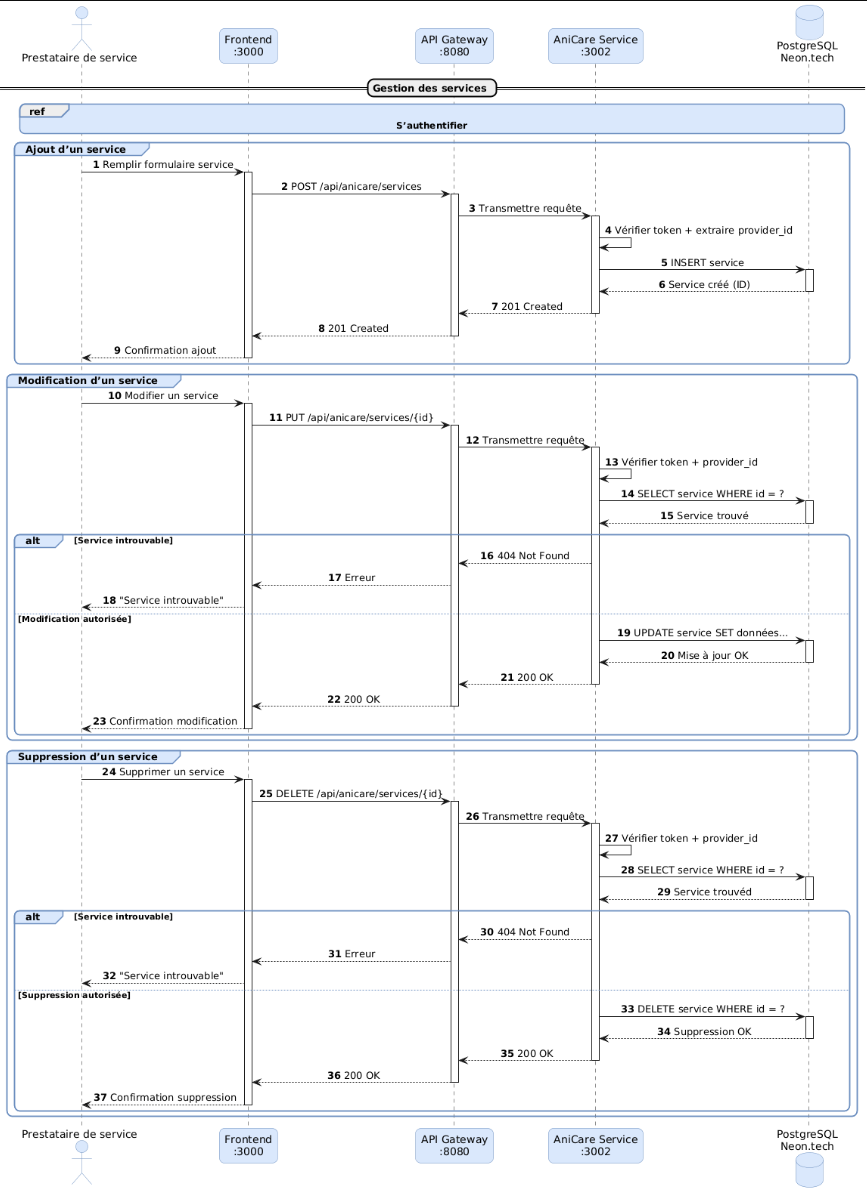
\includegraphics[width=0.8\textwidth]{images/gerer mes services sq.png}
    \caption{Diagramme de séquence : gestion des services}
    \label{fig:services_prestataire}
\end{figure}
\newpage 
\subsubsection{Diagramme de séquence : gestion des réservations reçues}

Cette figure illustre les interactions du prestataire de service pour la consultation, l’acceptation ou le refus des réservations reçues, ainsi que l’affichage de son emploi du temps. Elle met en évidence les échanges entre le frontend, l’API Gateway, le service AniCare, la base de données et le système de notification : 

\begin{figure}[H]
    \centering
    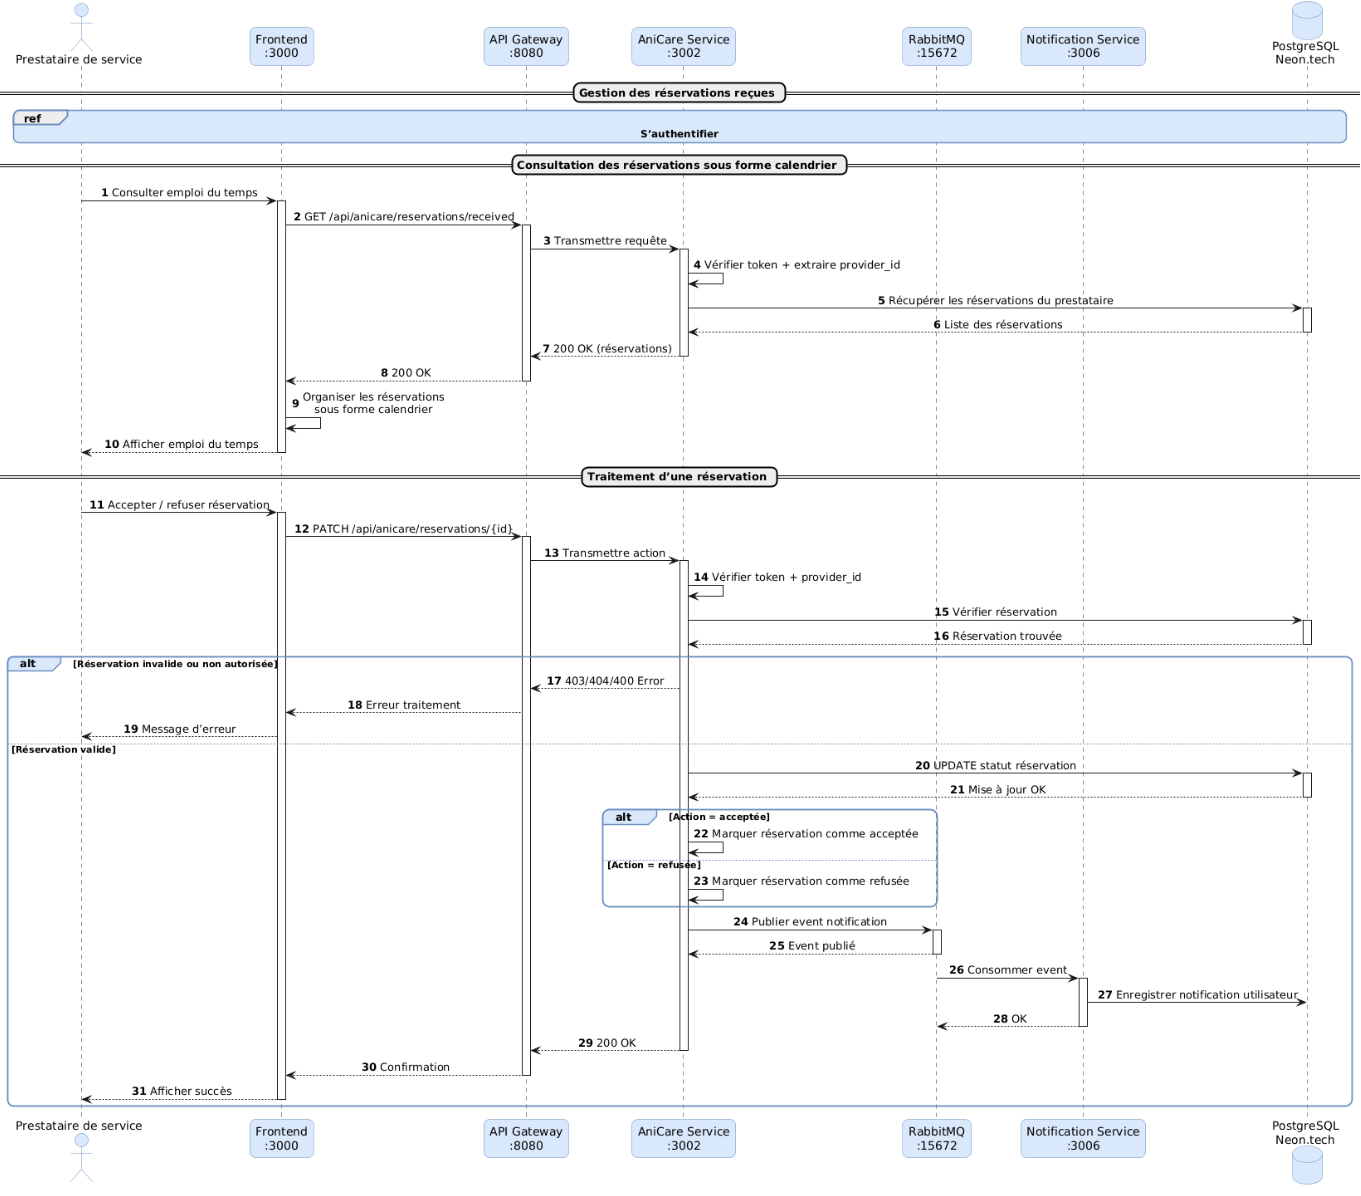
\includegraphics[width=1\textwidth]{images/gerer reservations recus sq.png}
    \caption{Diagramme de séquence : gestion des réservations reçues}
    \label{fig:reservations_prestataire}
\end{figure}
\newpage
\subsection{Réalisation du sprint 5} 
\subsubsection{Interface d’accueil AniCare} 
Cette figure illustre l’interface d’accueil du
module AniCare :  
\begin{figure}[h!]
    \centering
    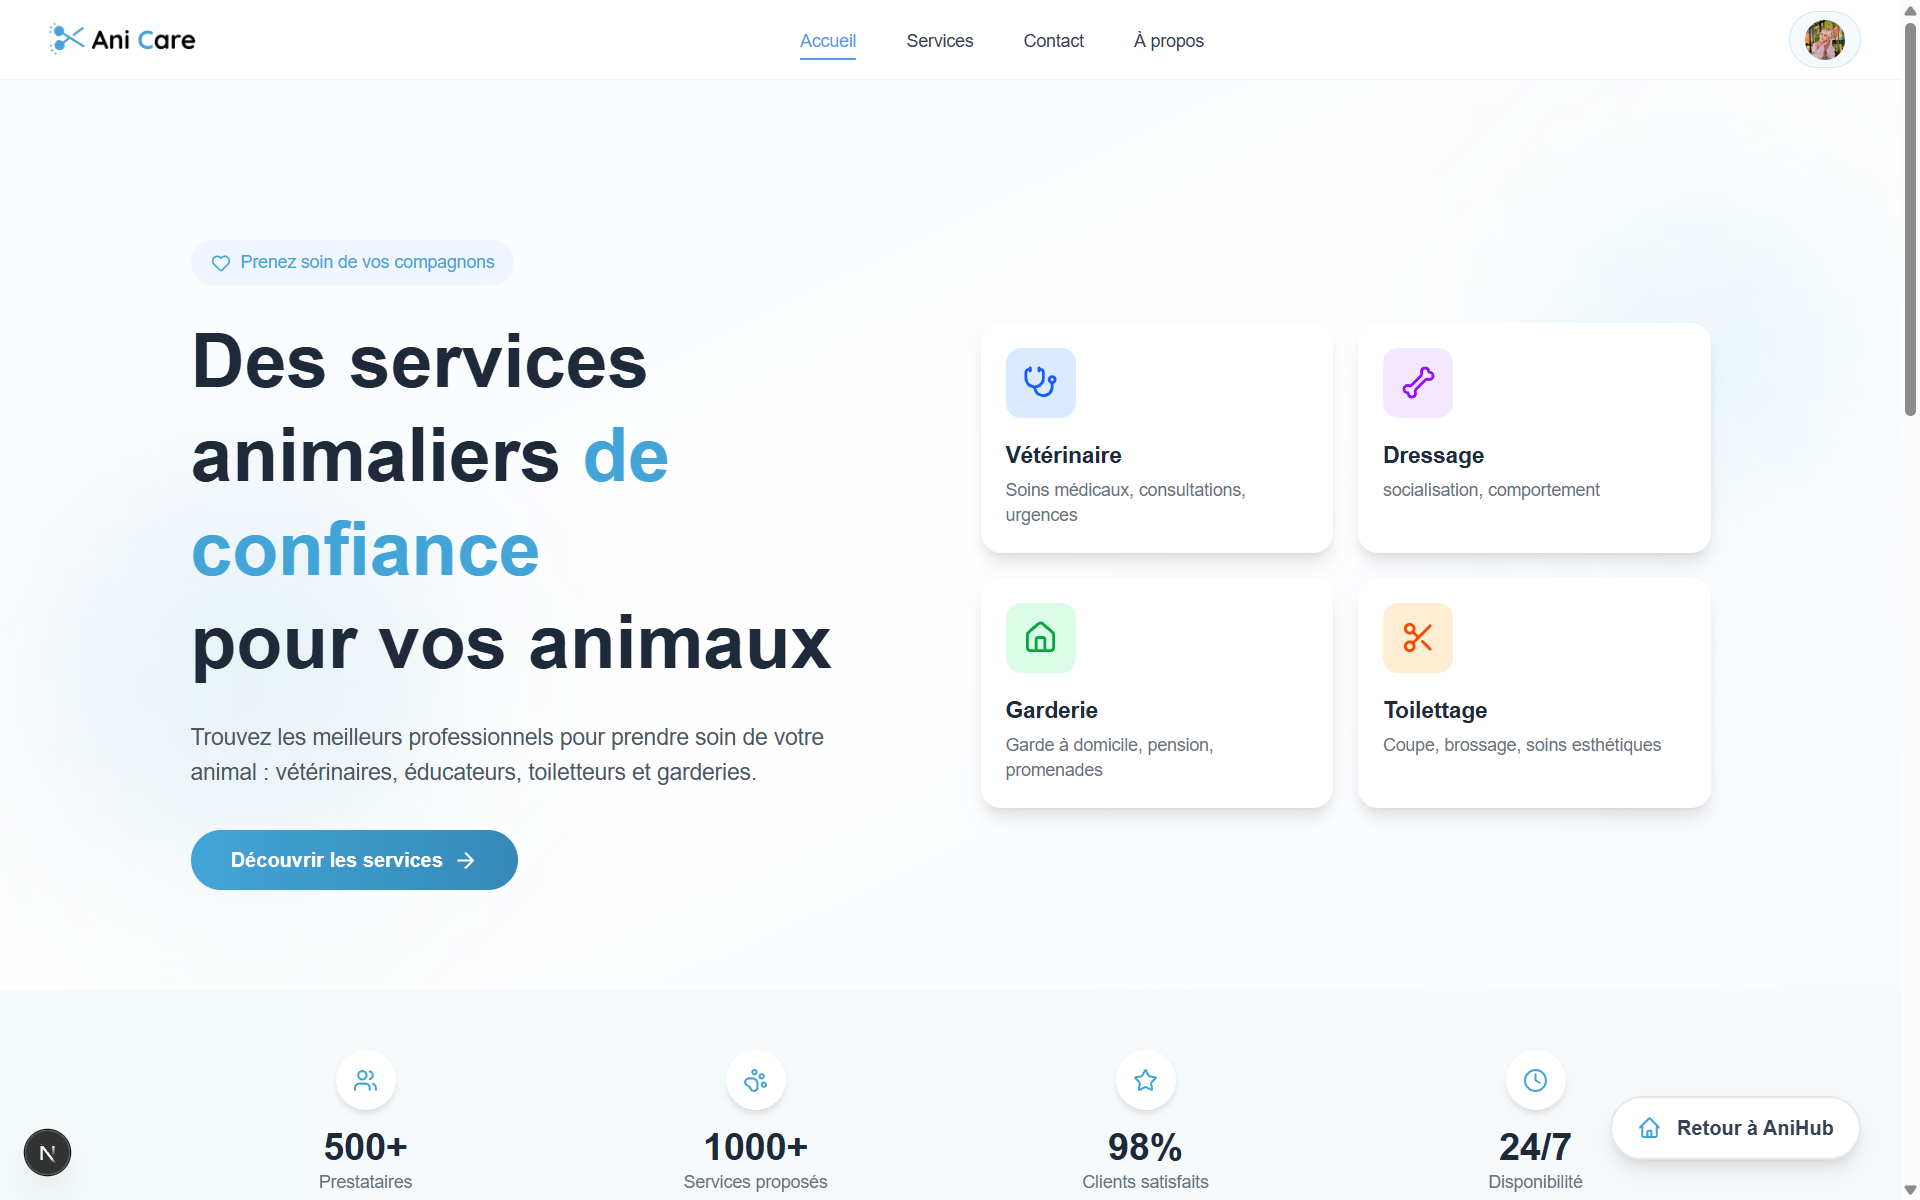
\includegraphics[width=0.73\textwidth]{images/acceuil anicare.png}
    \caption{Interface d’accueil du module AniCare}
\end{figure}  
\subsubsection{Interface de publication d’un service}   
Cette interface illustre le formulaire de publication d’un service dans le module AniCare : 
\begin{figure}[h!]
    \centering
    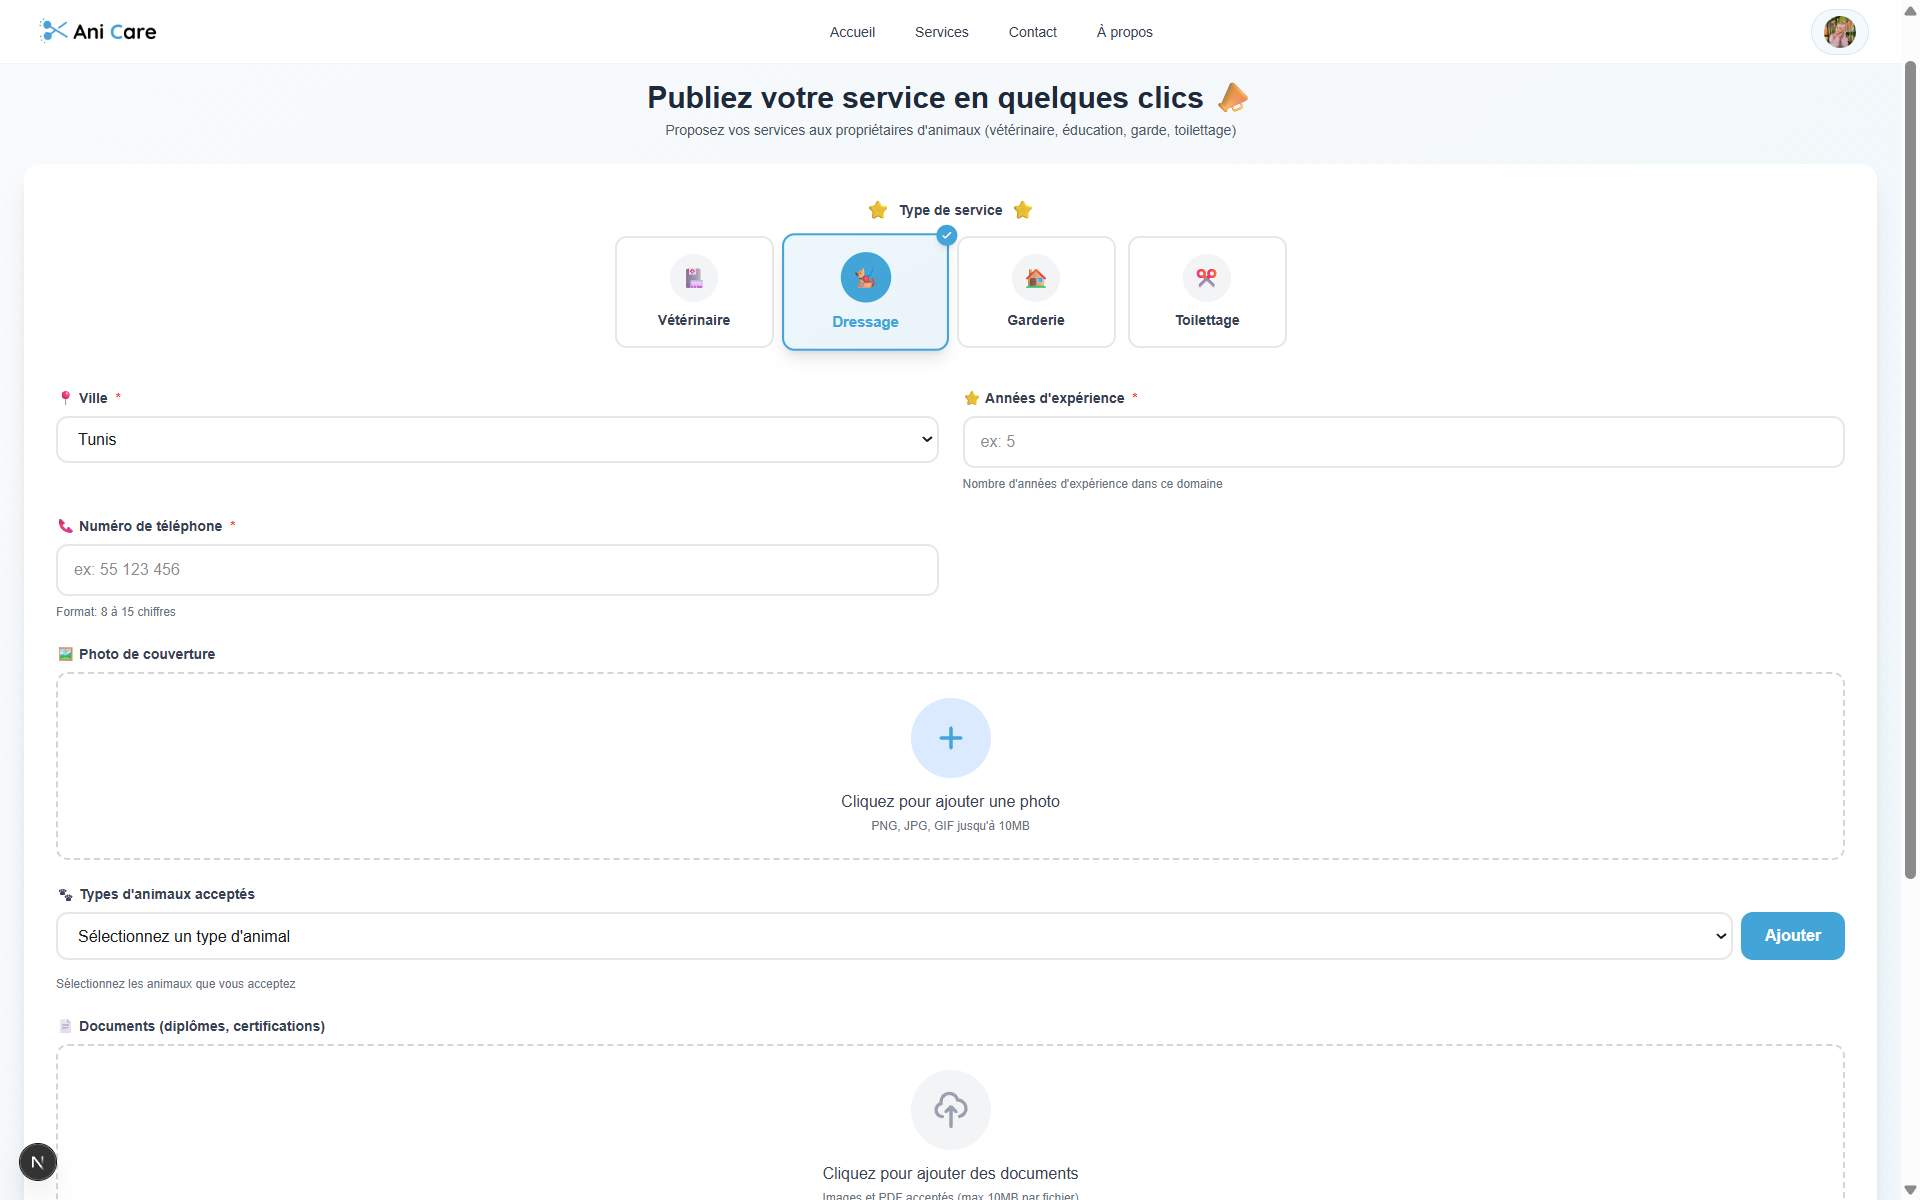
\includegraphics[width=0.73\textwidth]{images/publier mon service.png}
    \caption{Interface de publication d’un service}
\end{figure}  
\newpage 

\subsubsection{Interface des annonces de services dans AniCare}  
Cette interface illustre les services proposés par les prestataires dans le module AniCare : 
\begin{figure}[h!]
    \centering
    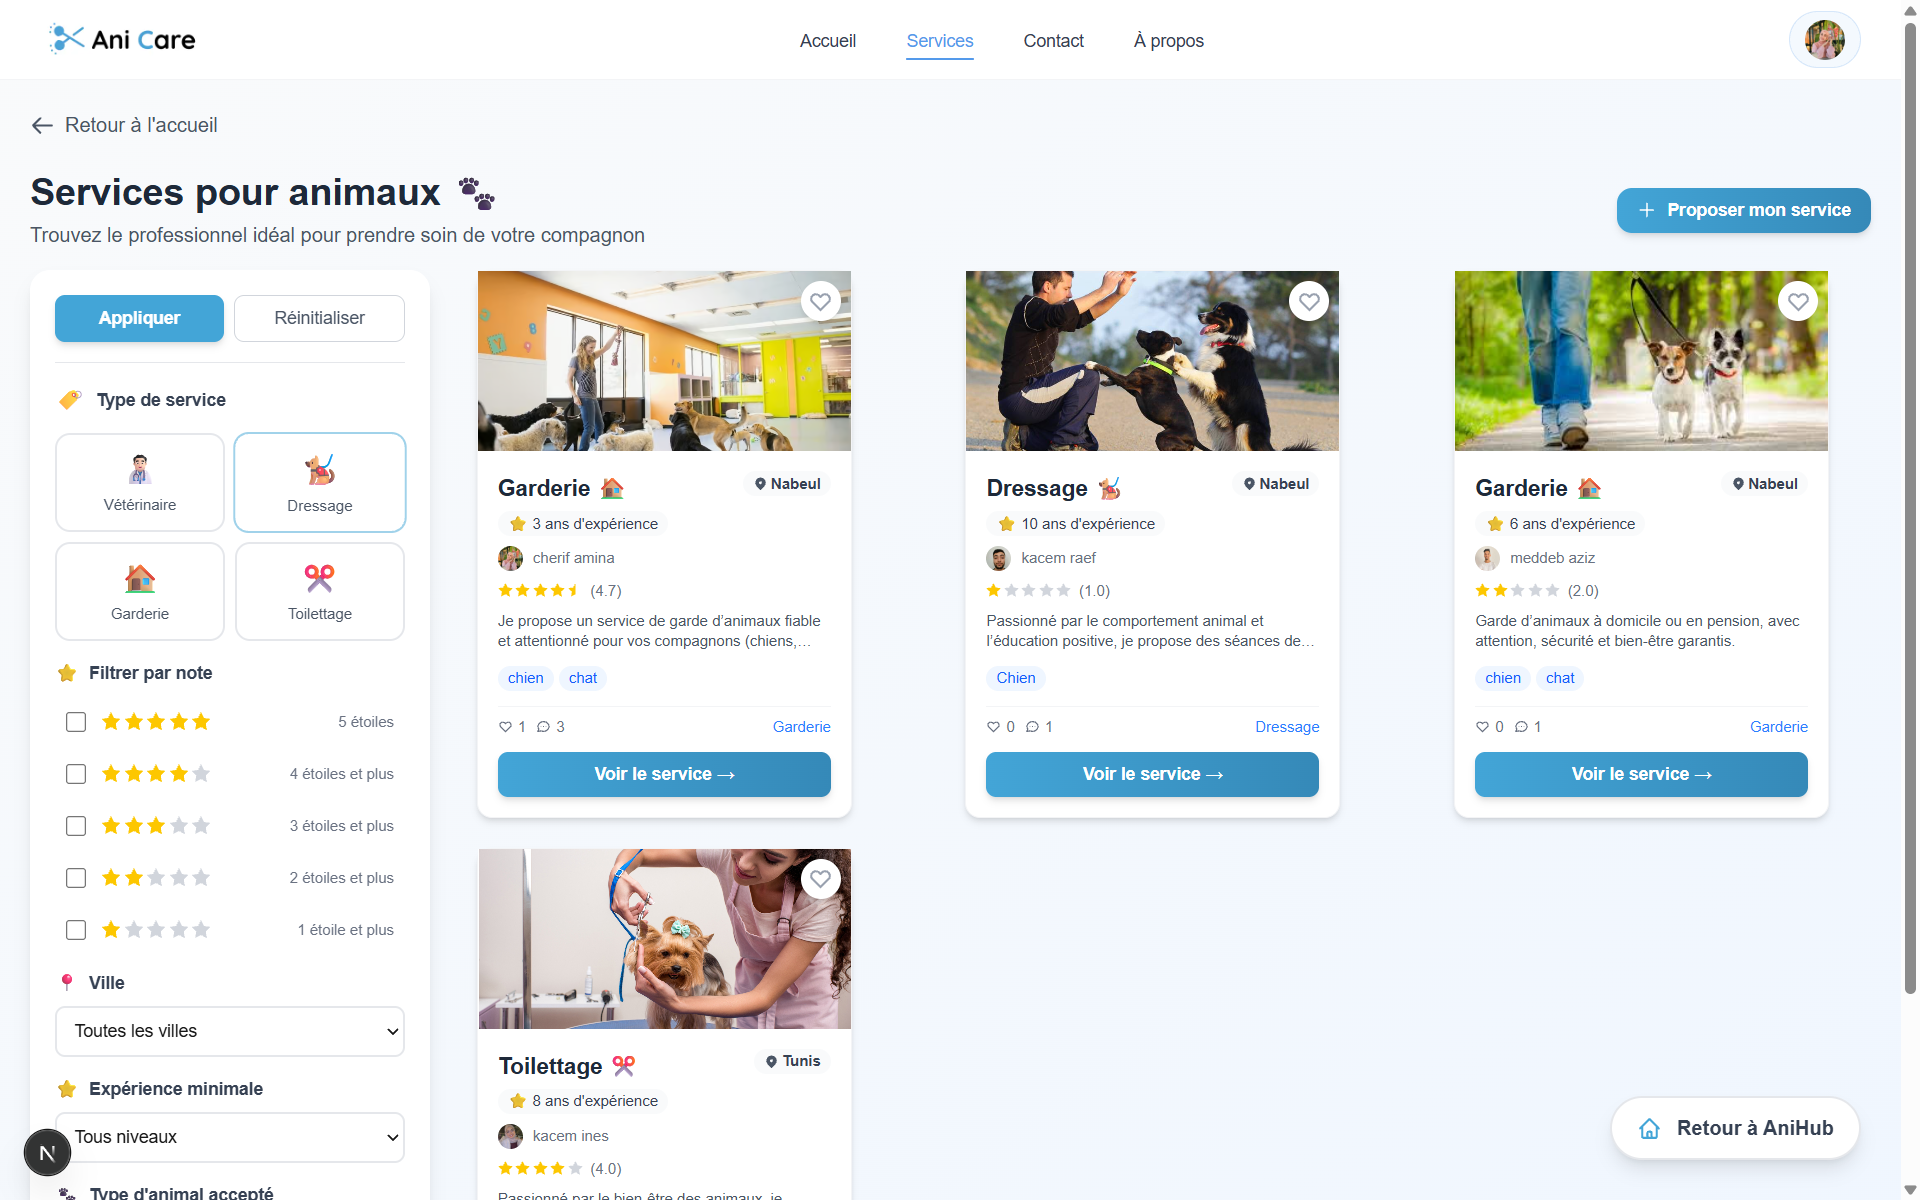
\includegraphics[width=0.73\textwidth]{images/services.png}
    \caption{Interface des annonces de services dans AniCare}
\end{figure}   

\subsubsection{Interface des détails d’un service} 
Cette interface illustre les détails d’un service proposé dans le module AniCare : 
\begin{figure}[h!]
    \centering
    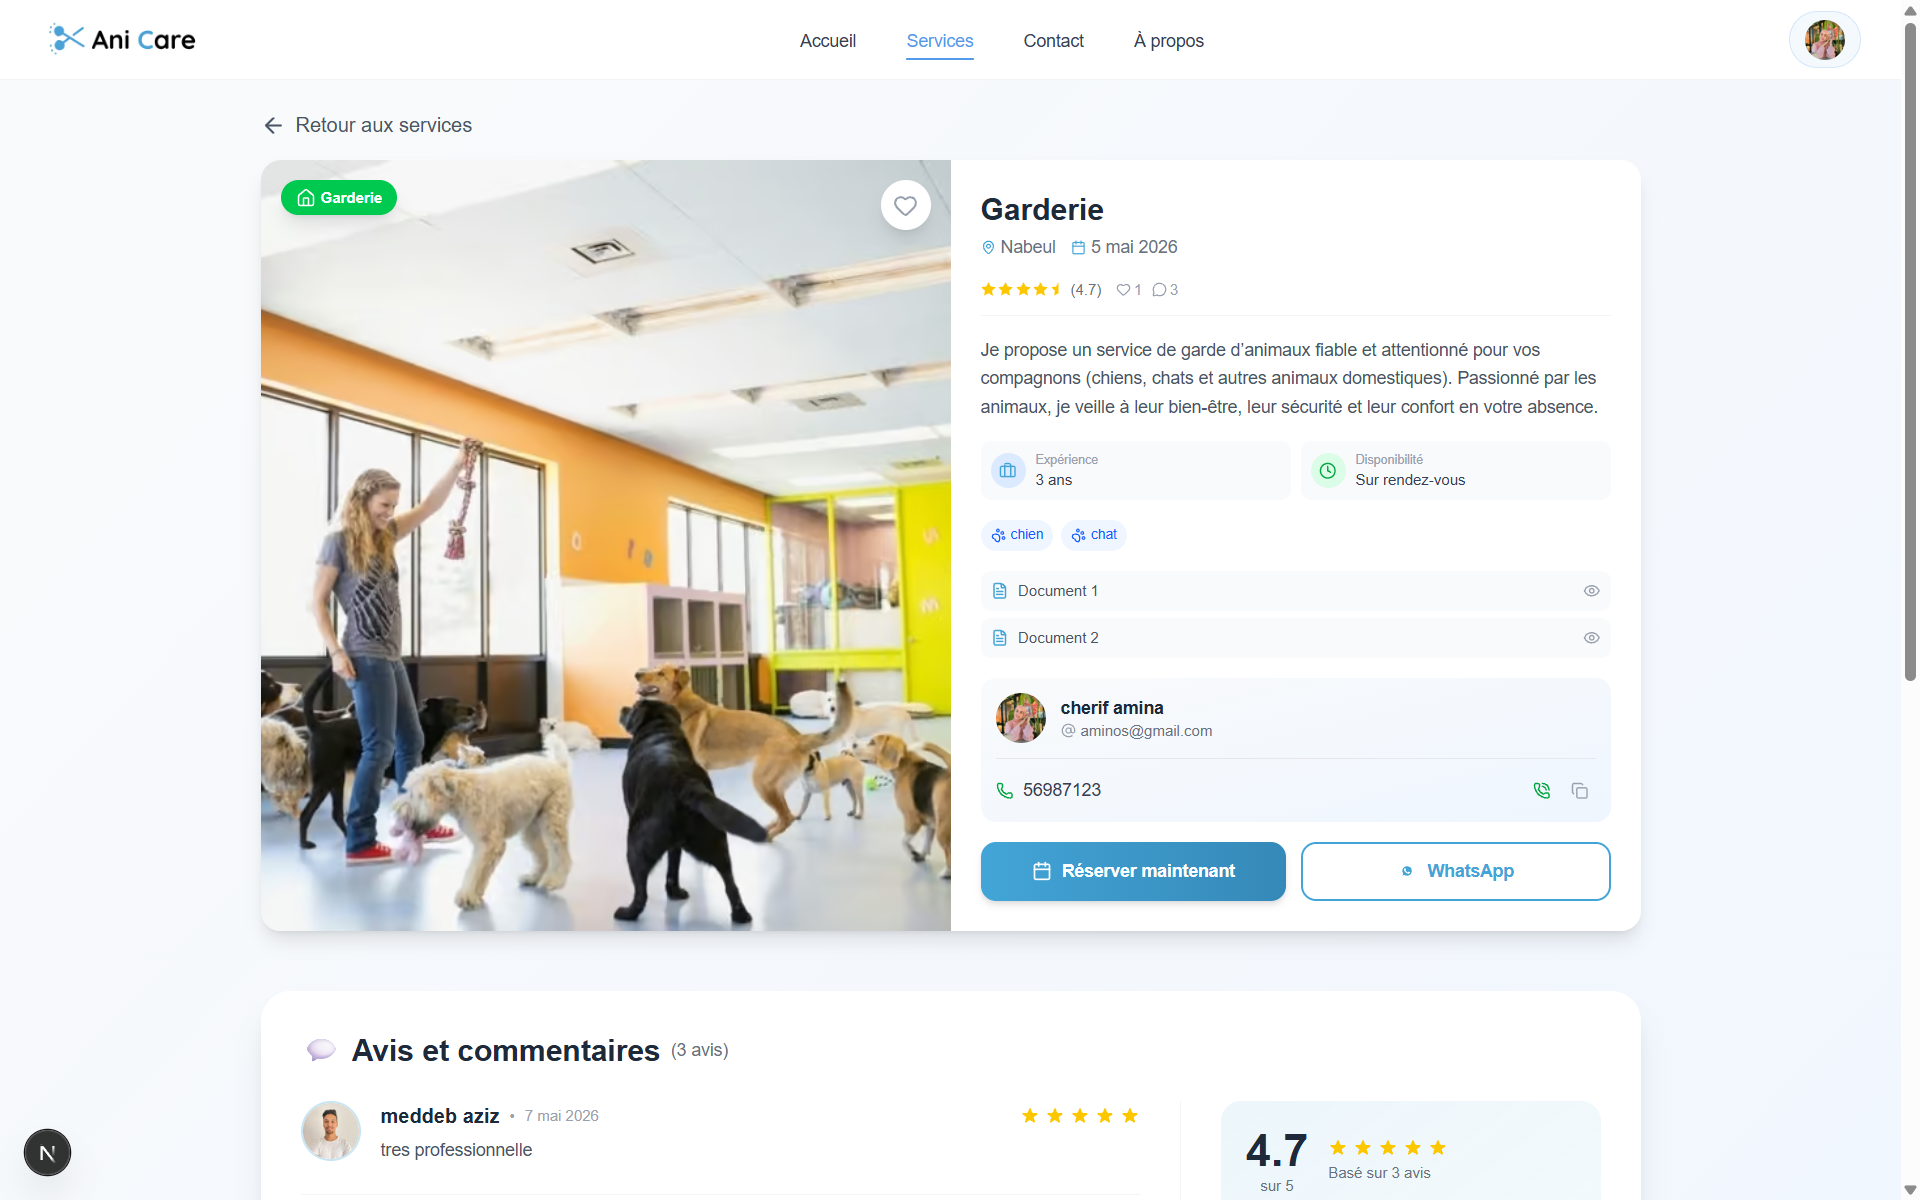
\includegraphics[width=0.73\textwidth]{images/details services.png}
    \caption{Interface des détails d’un service}
\end{figure}   
\newpage 
\subsubsection{Interface de réservation d’un service pour un demandeur} 
Cette interface illustre le processus de réservation d’un service par un demandeur dans le module AniCare : 
\begin{figure}[h!]
    \centering
    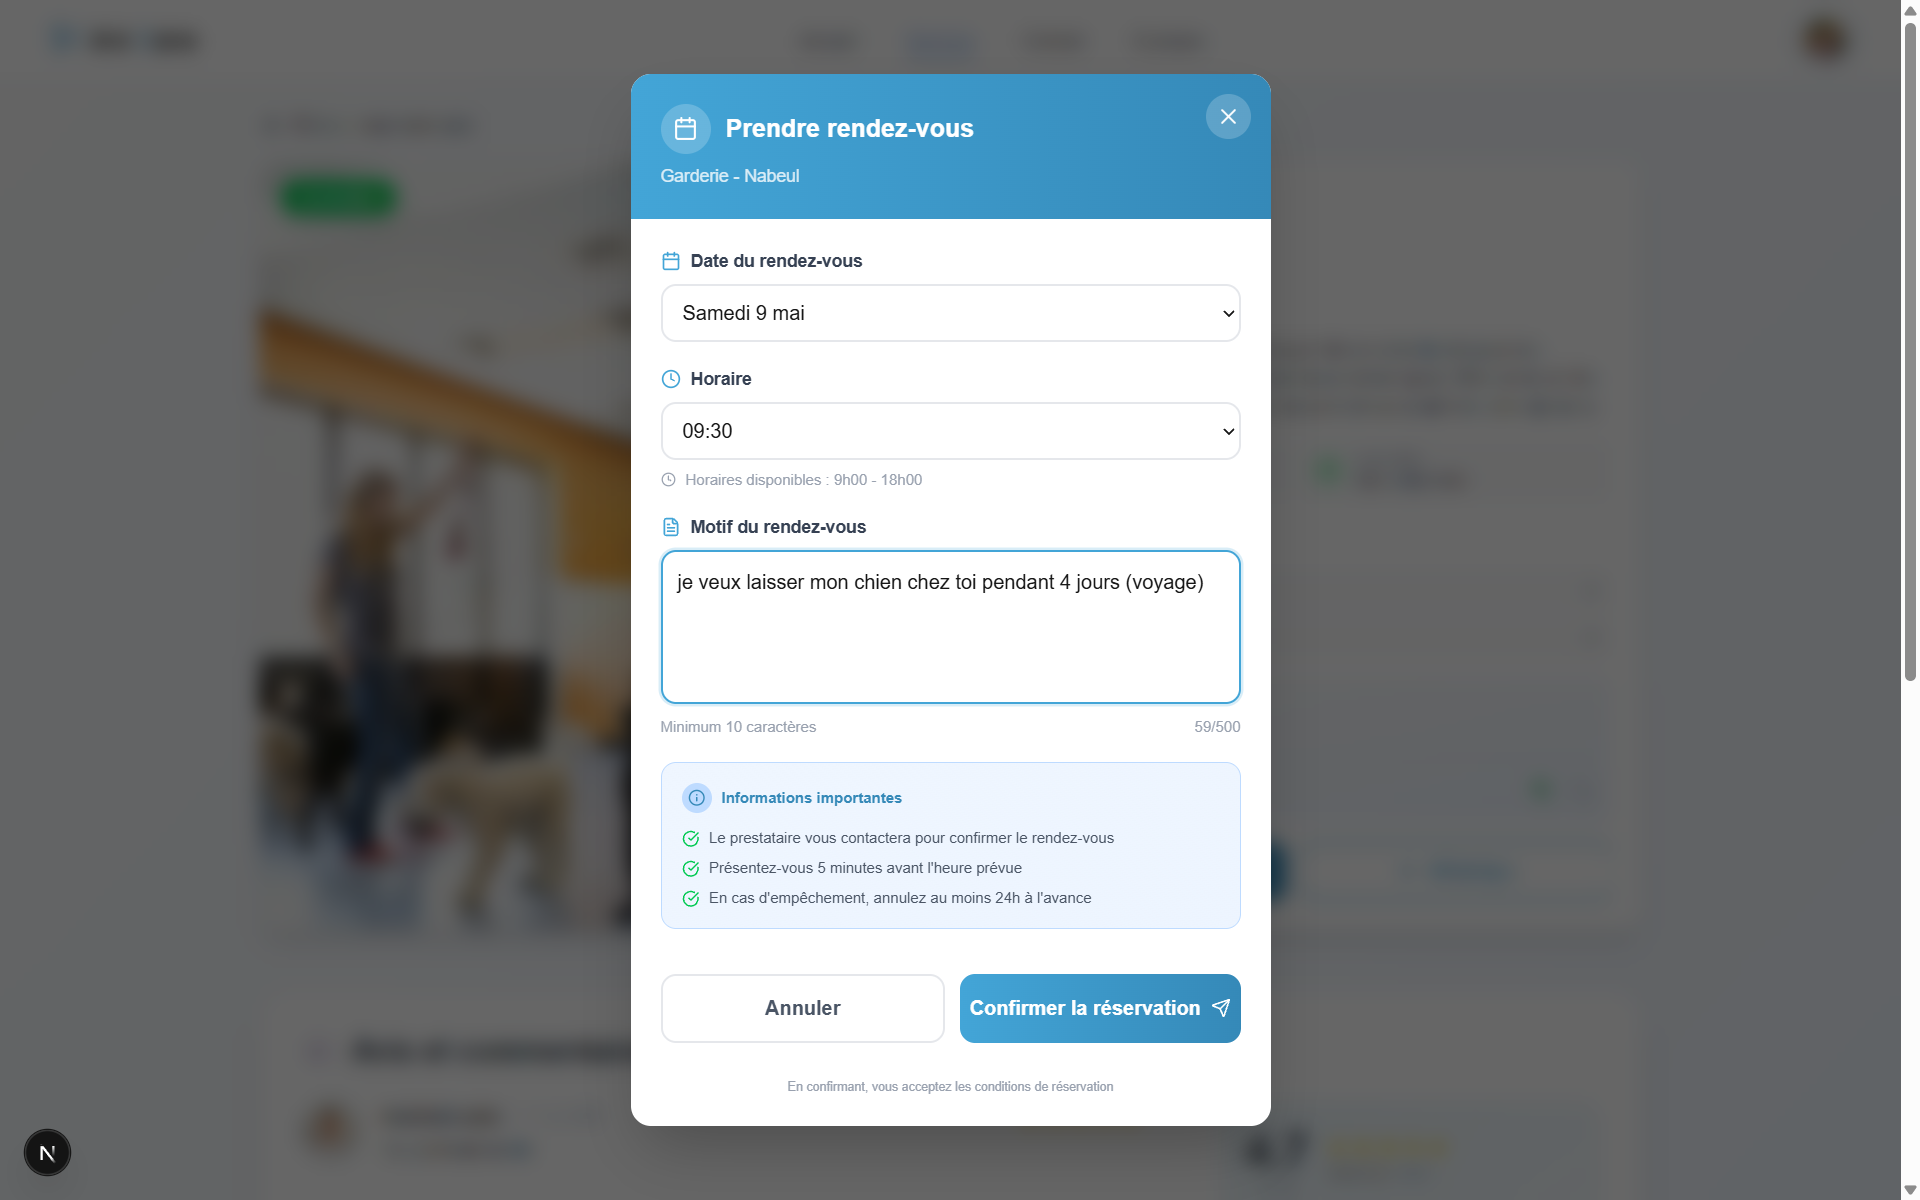
\includegraphics[width=0.73\textwidth]{images/interface reservation.png}
    \caption{Interface de réservation d’un service pour un demandeur}
\end{figure}   

\subsubsection{Interface des avis des clients sur un service}  
Cette interface illustre les avis et évaluations laissés par les clients pour un service dans le module AniCare : 

\begin{figure}[h!]
    \centering
    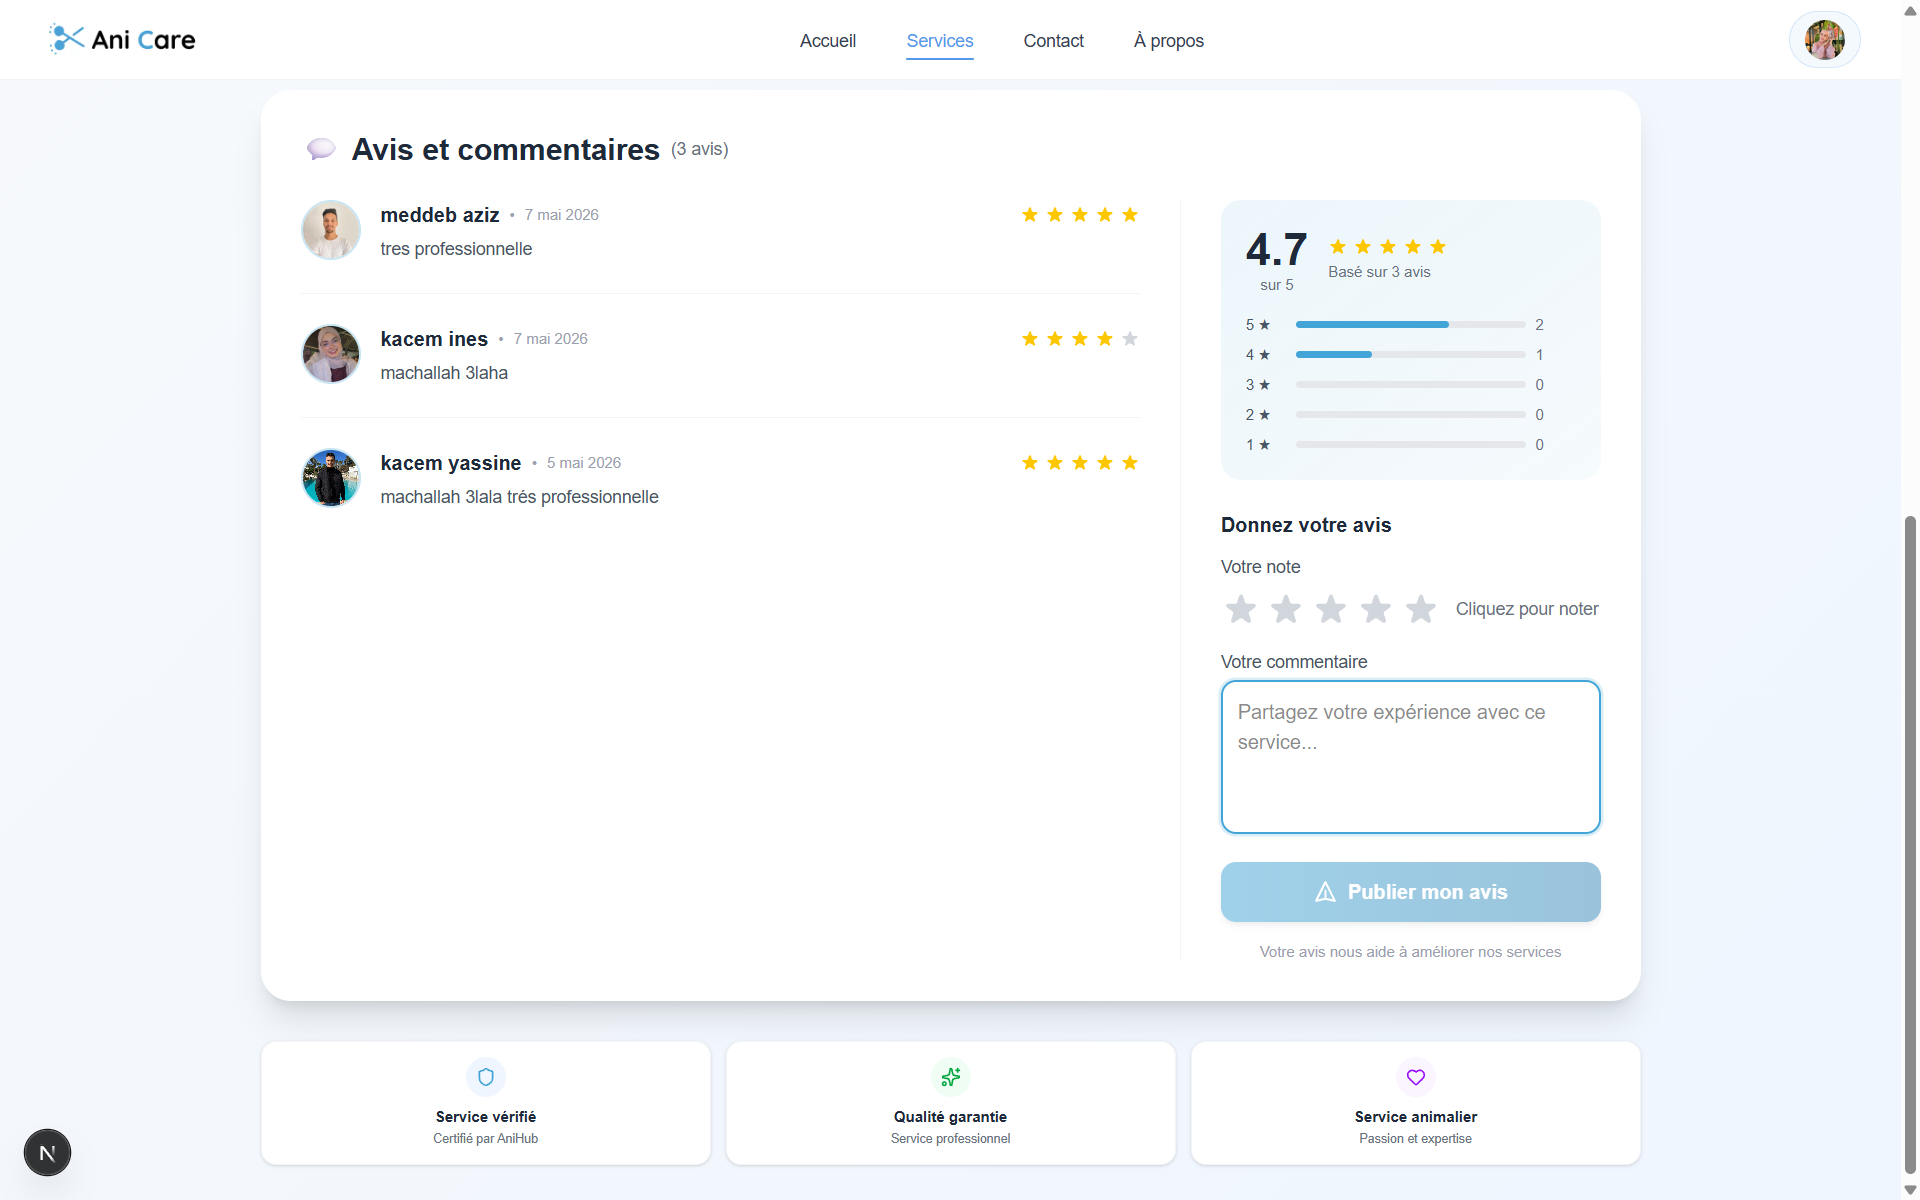
\includegraphics[width=0.73\textwidth]{images/interface avis.png}
    \caption{Interface des avis des clients sur un service}
\end{figure}  
\newpage 
\subsubsection{Interface de l’espace AniCare pour un prestataire} 
Cette interface illustre l’espace personnel du prestataire dans le module AniCare, lui permettant de gérer ses services et ses réservations : 
\begin{figure}[h!]
    \centering
    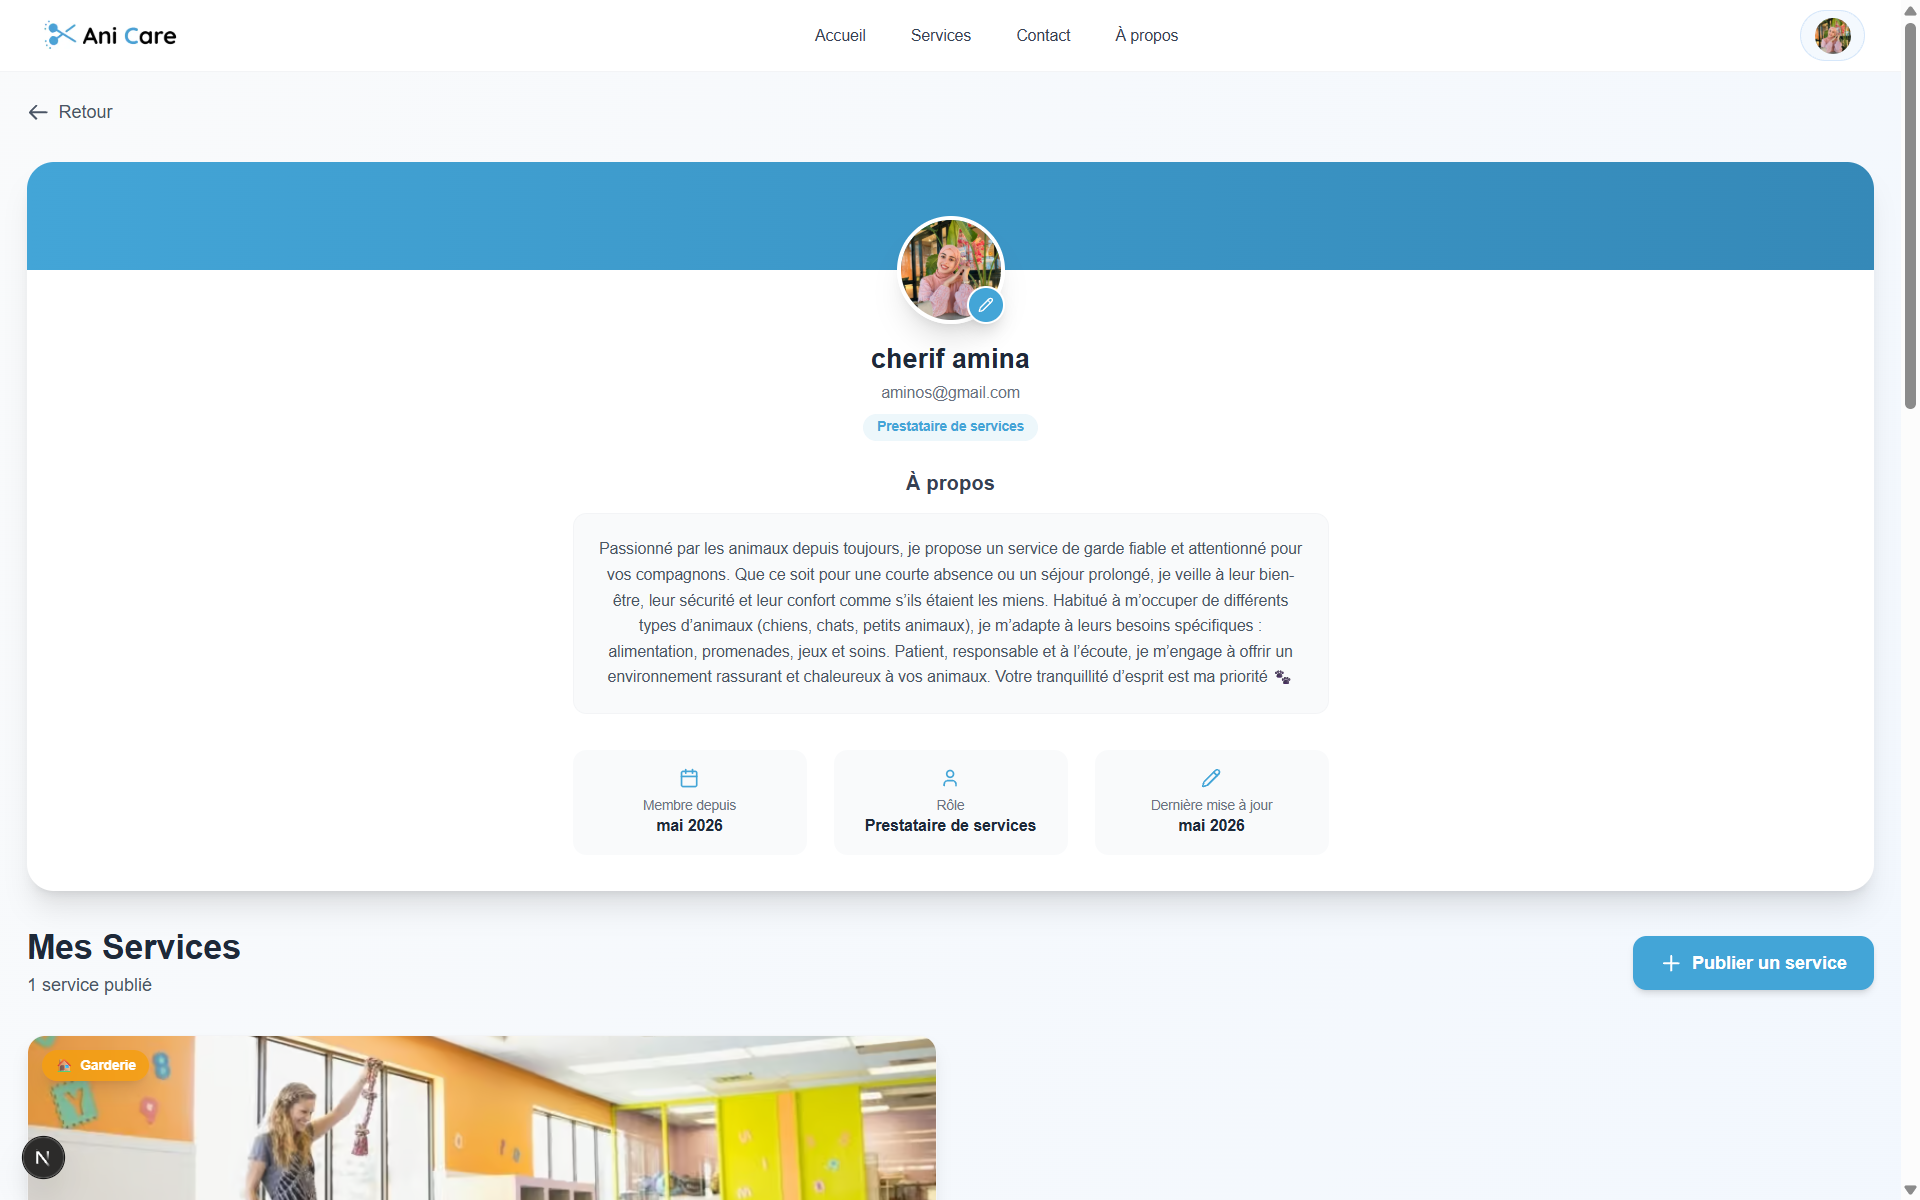
\includegraphics[width=0.73\textwidth]{images/espace anicare.png}
    \caption{Interface de l’espace AniCare pour un prestataire}
\end{figure}    
\subsubsection{Interfaces de modification et de suppression d’un service} 
Ces interfaces illustrent les fonctionnalités de modification et de suppression d’un service dans le module AniCare : 
\begin{figure}[h!]
    \centering
    
    \begin{minipage}{0.48\textwidth}
        \centering
        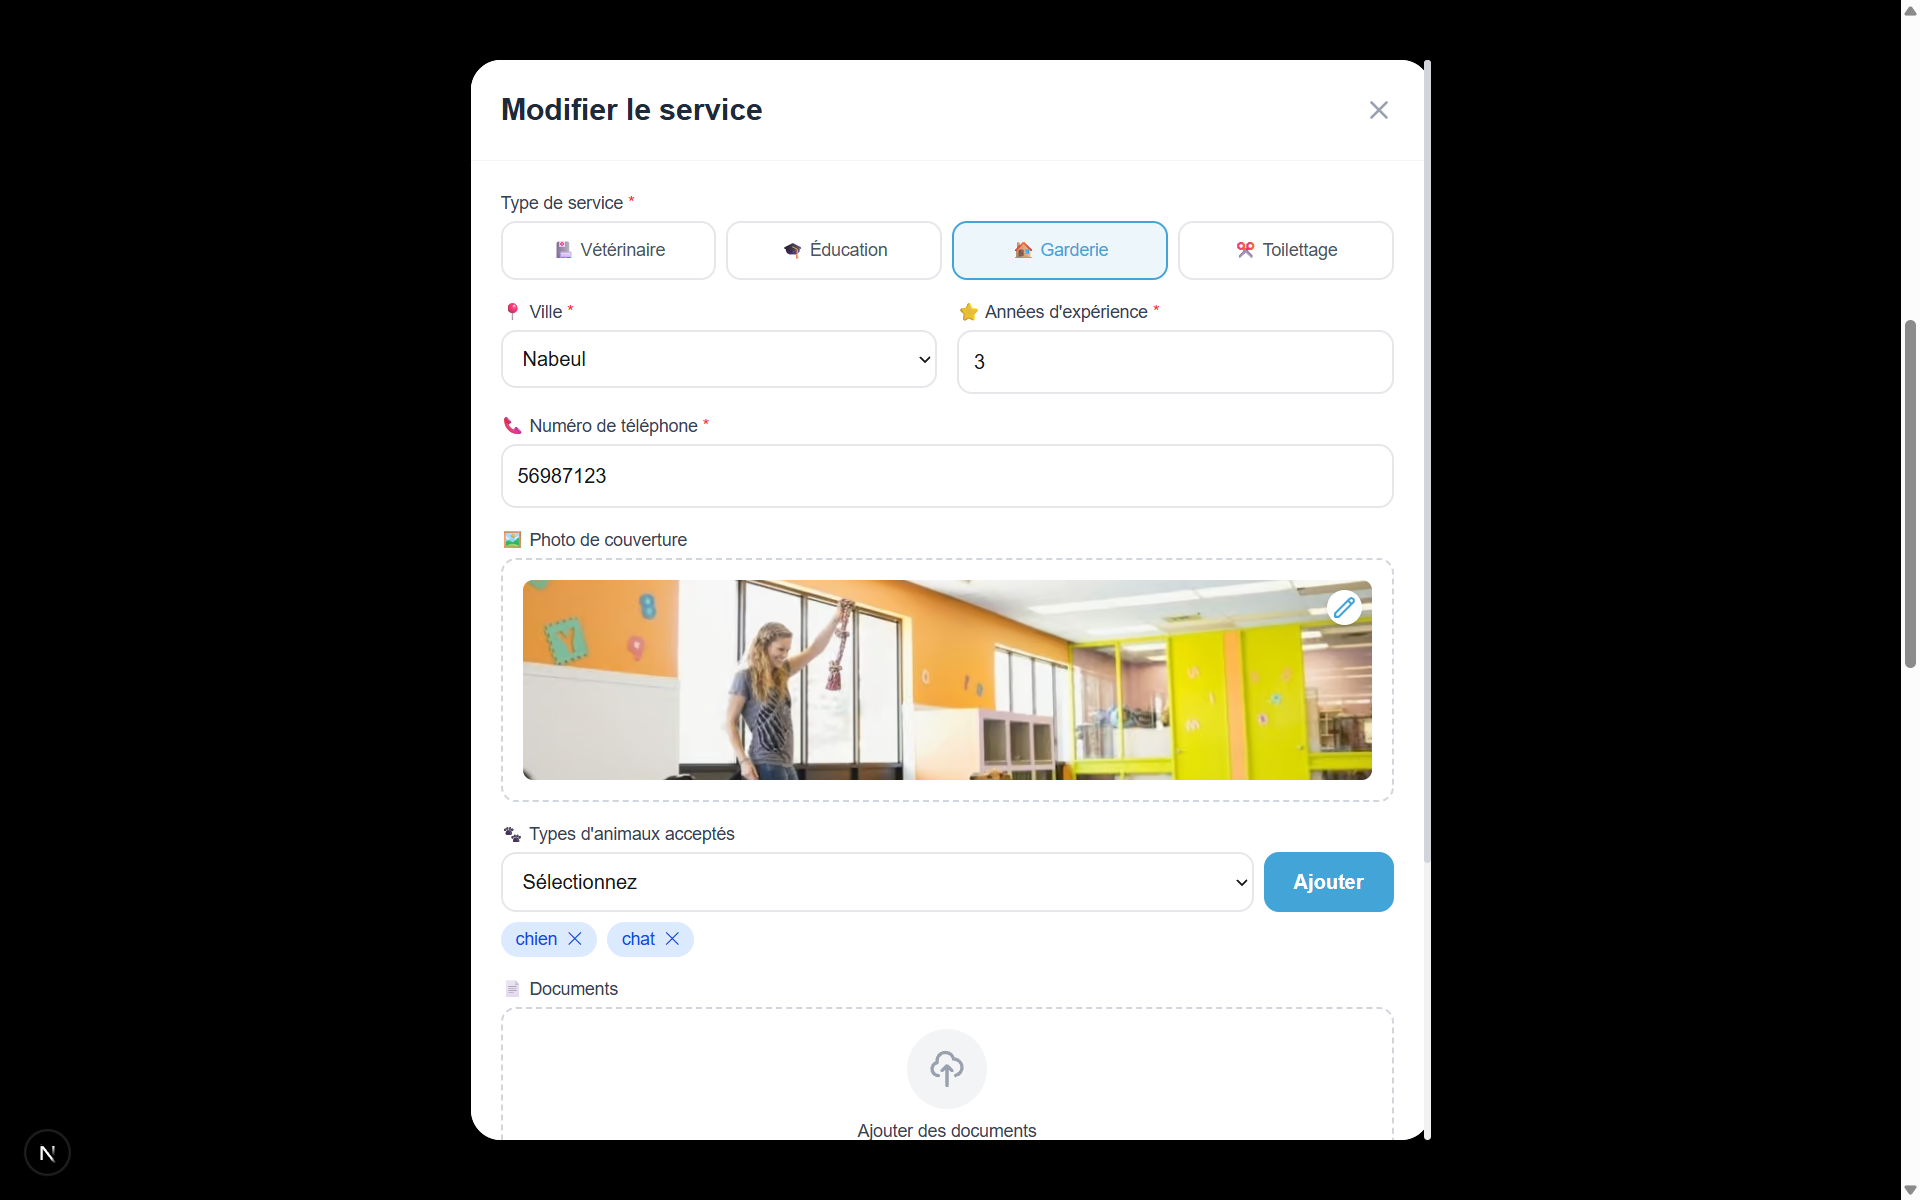
\includegraphics[width=\textwidth]{images/modifieer service.png}
        \caption{Interface modification service}
    \end{minipage}
    \hfill
    \begin{minipage}{0.48\textwidth}
        \centering
        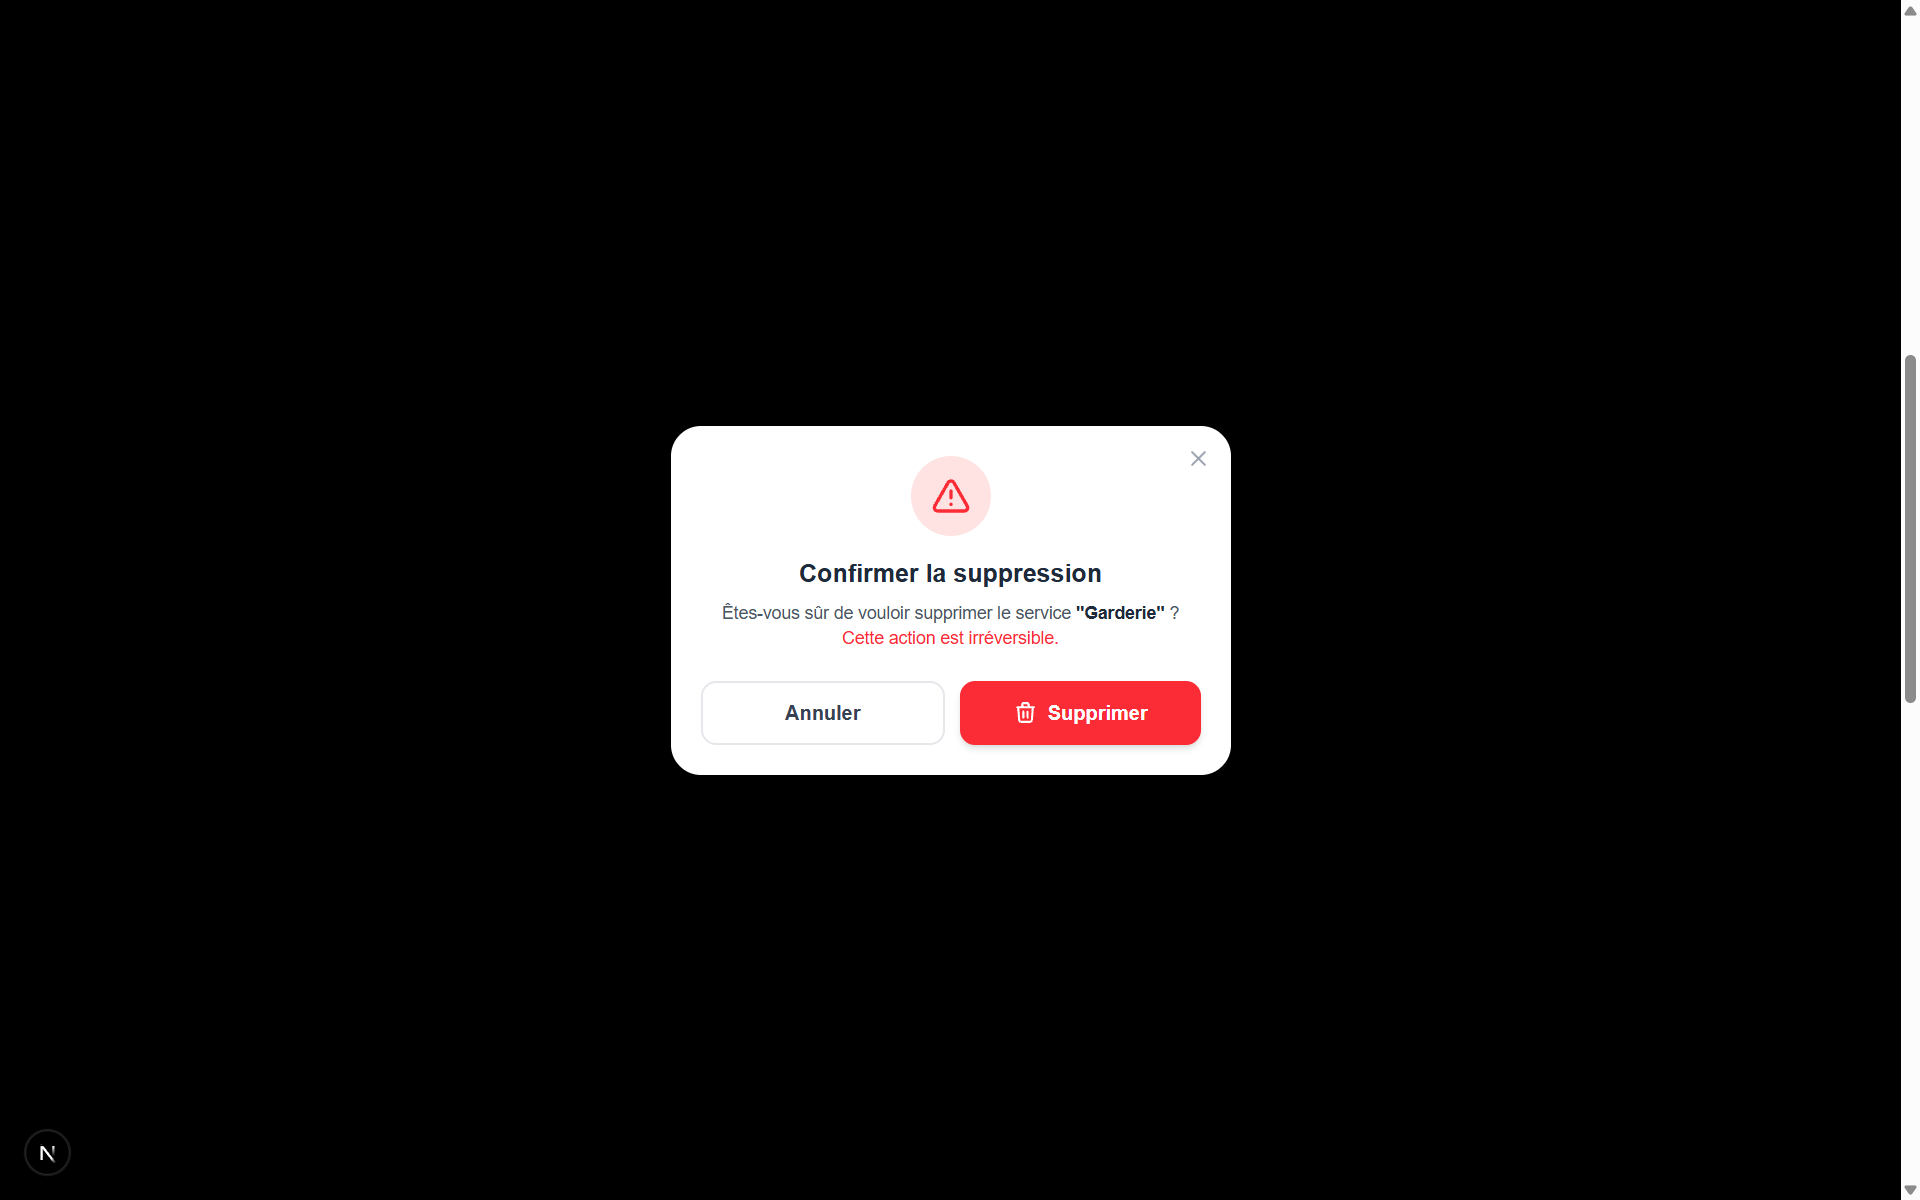
\includegraphics[width=\textwidth]{images/suppression service}
        \caption{Interface suppression service}
    \end{minipage}

\end{figure}  
\newpage 
\subsubsection{Interface de gestion des réservations reçues pour le prestataire} 
Cette interface illustre la gestion des réservations reçues par le prestataire dans le module AniCare : 
\begin{figure}[h!]
    \centering
    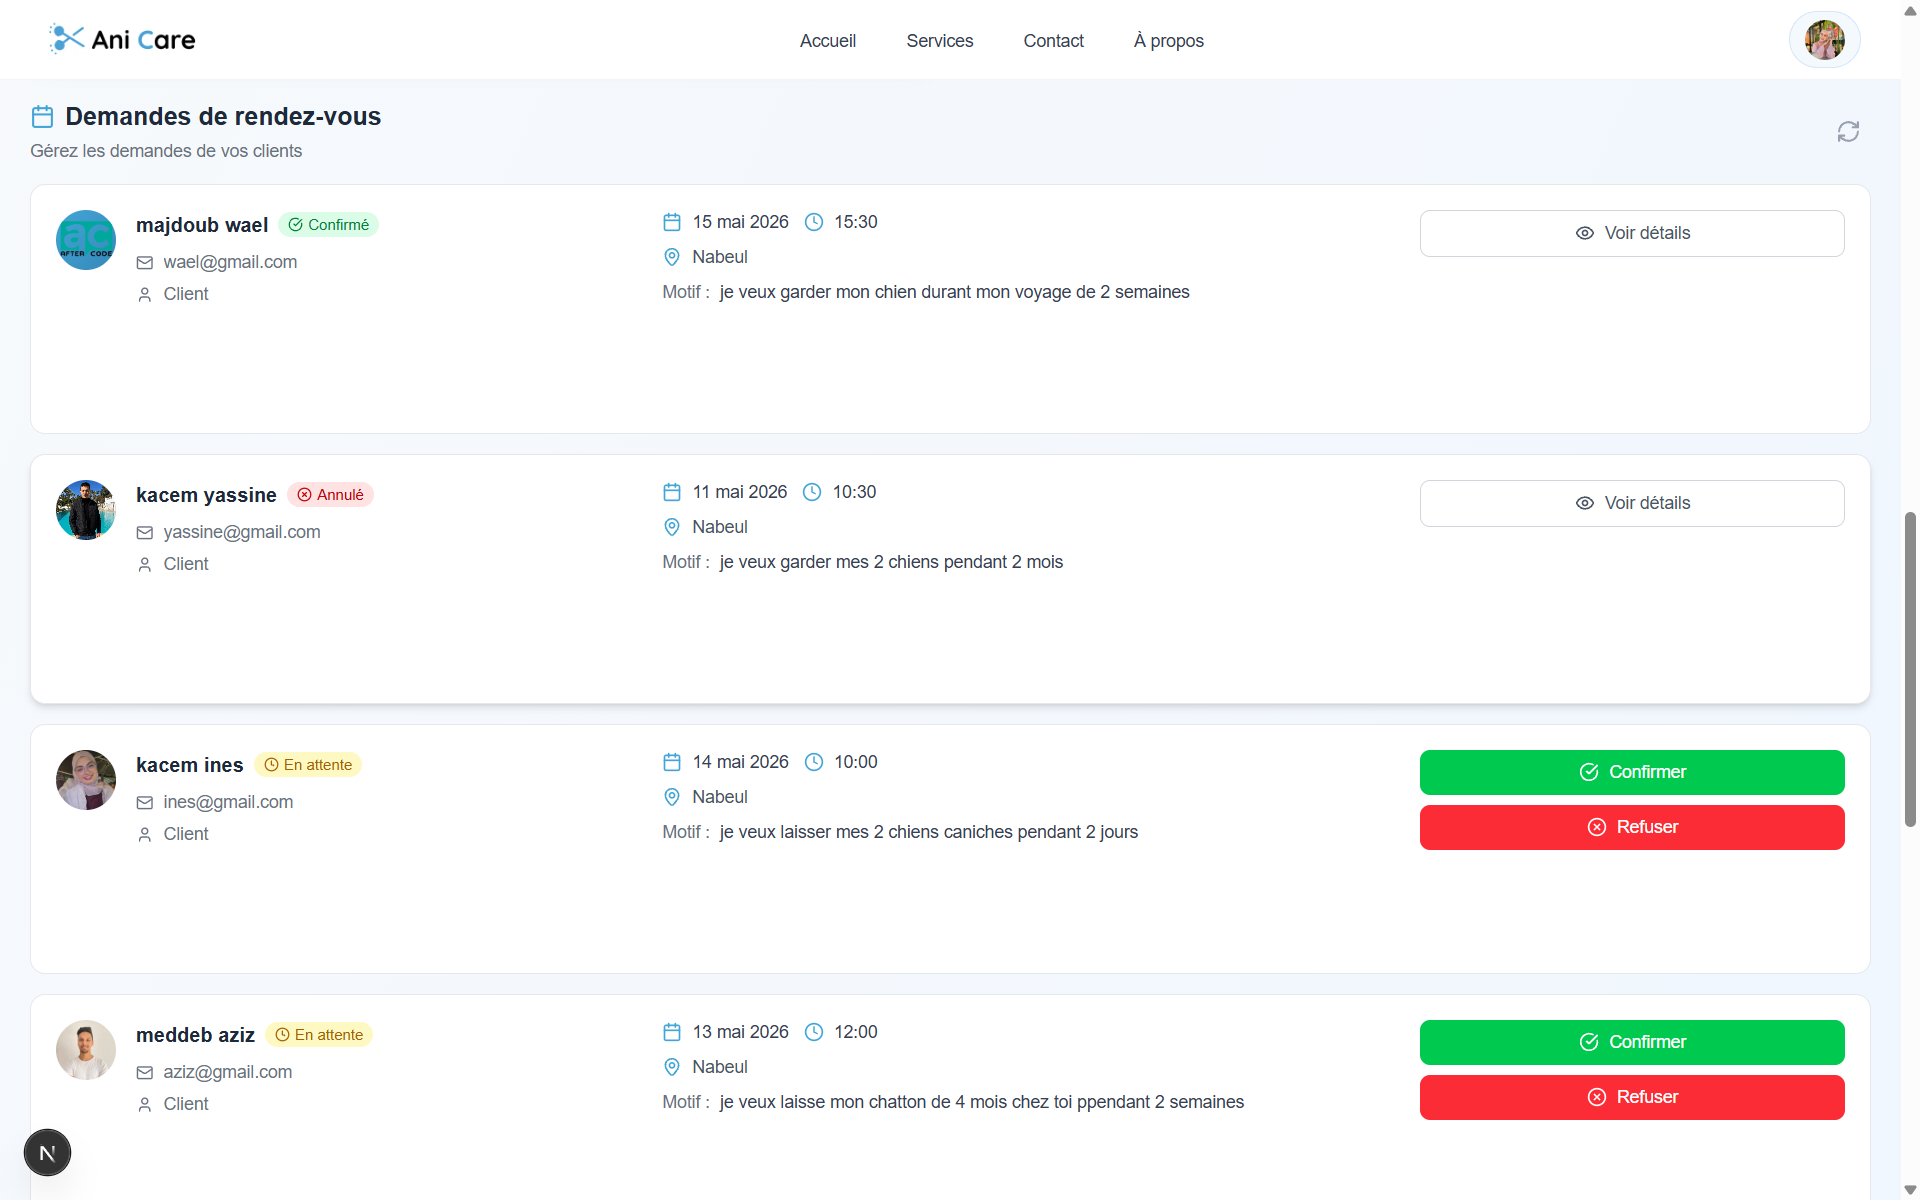
\includegraphics[width=0.73\textwidth]{images/mes reservation recus.png}
    \caption{Interface de gestion des réservations reçues pour le prestataire}
\end{figure}   
\subsubsection{Interface du planning du prestataire} 
Cette interface illustre le planning du prestataire dans le module AniCare, affichant ses horaires, jours et disponibilités : 
\begin{figure}[h!]
    \centering
    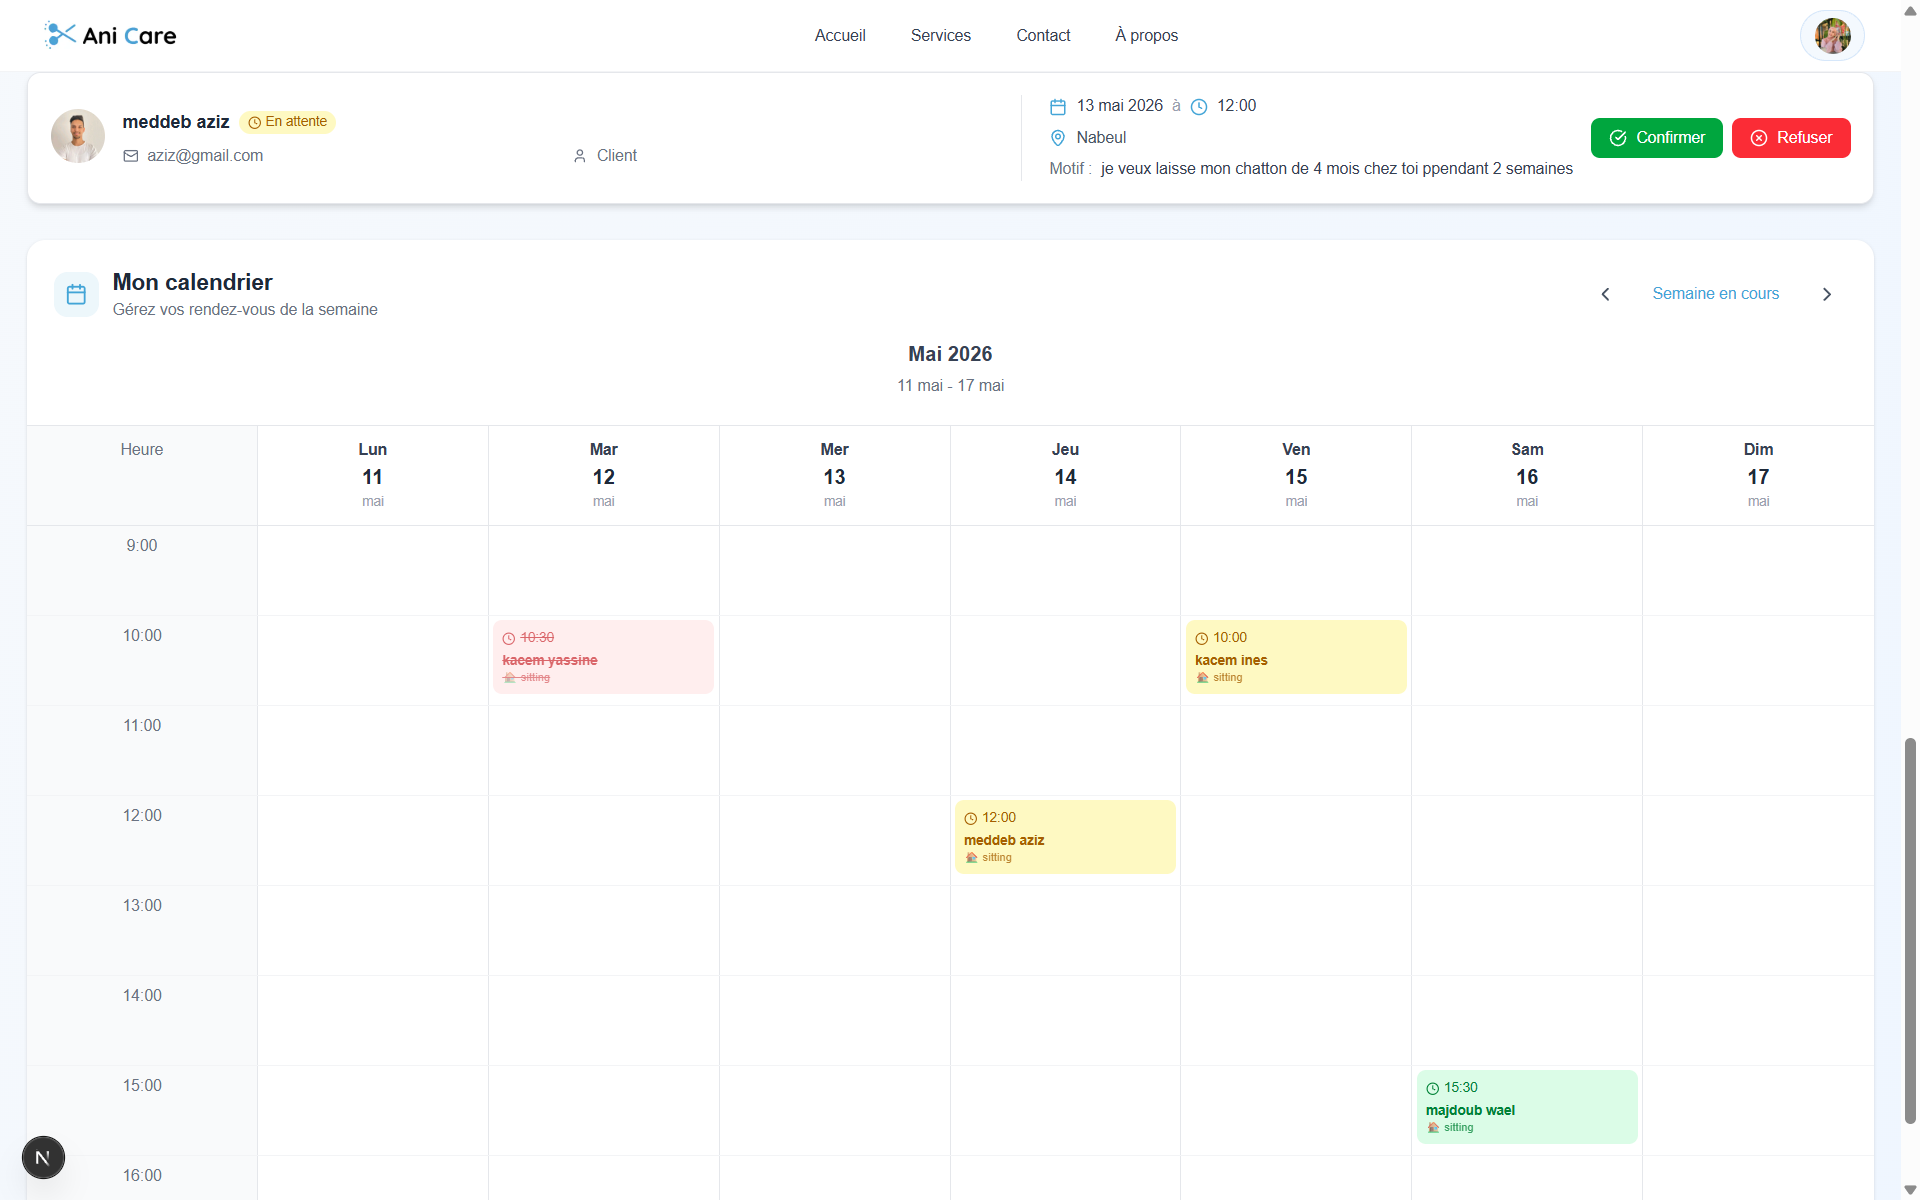
\includegraphics[width=0.73\textwidth]{images/mycalendar.png}
    \caption{Interface du planning du prestataire}
\end{figure}   
\newpage 
\subsubsection{Interface de gestion des réservations envoyées pour le demandeur} 
Cette interface illustre la gestion des réservations envoyées par le demandeur dans le module AniCare :
\begin{figure}[h!]
    \centering
    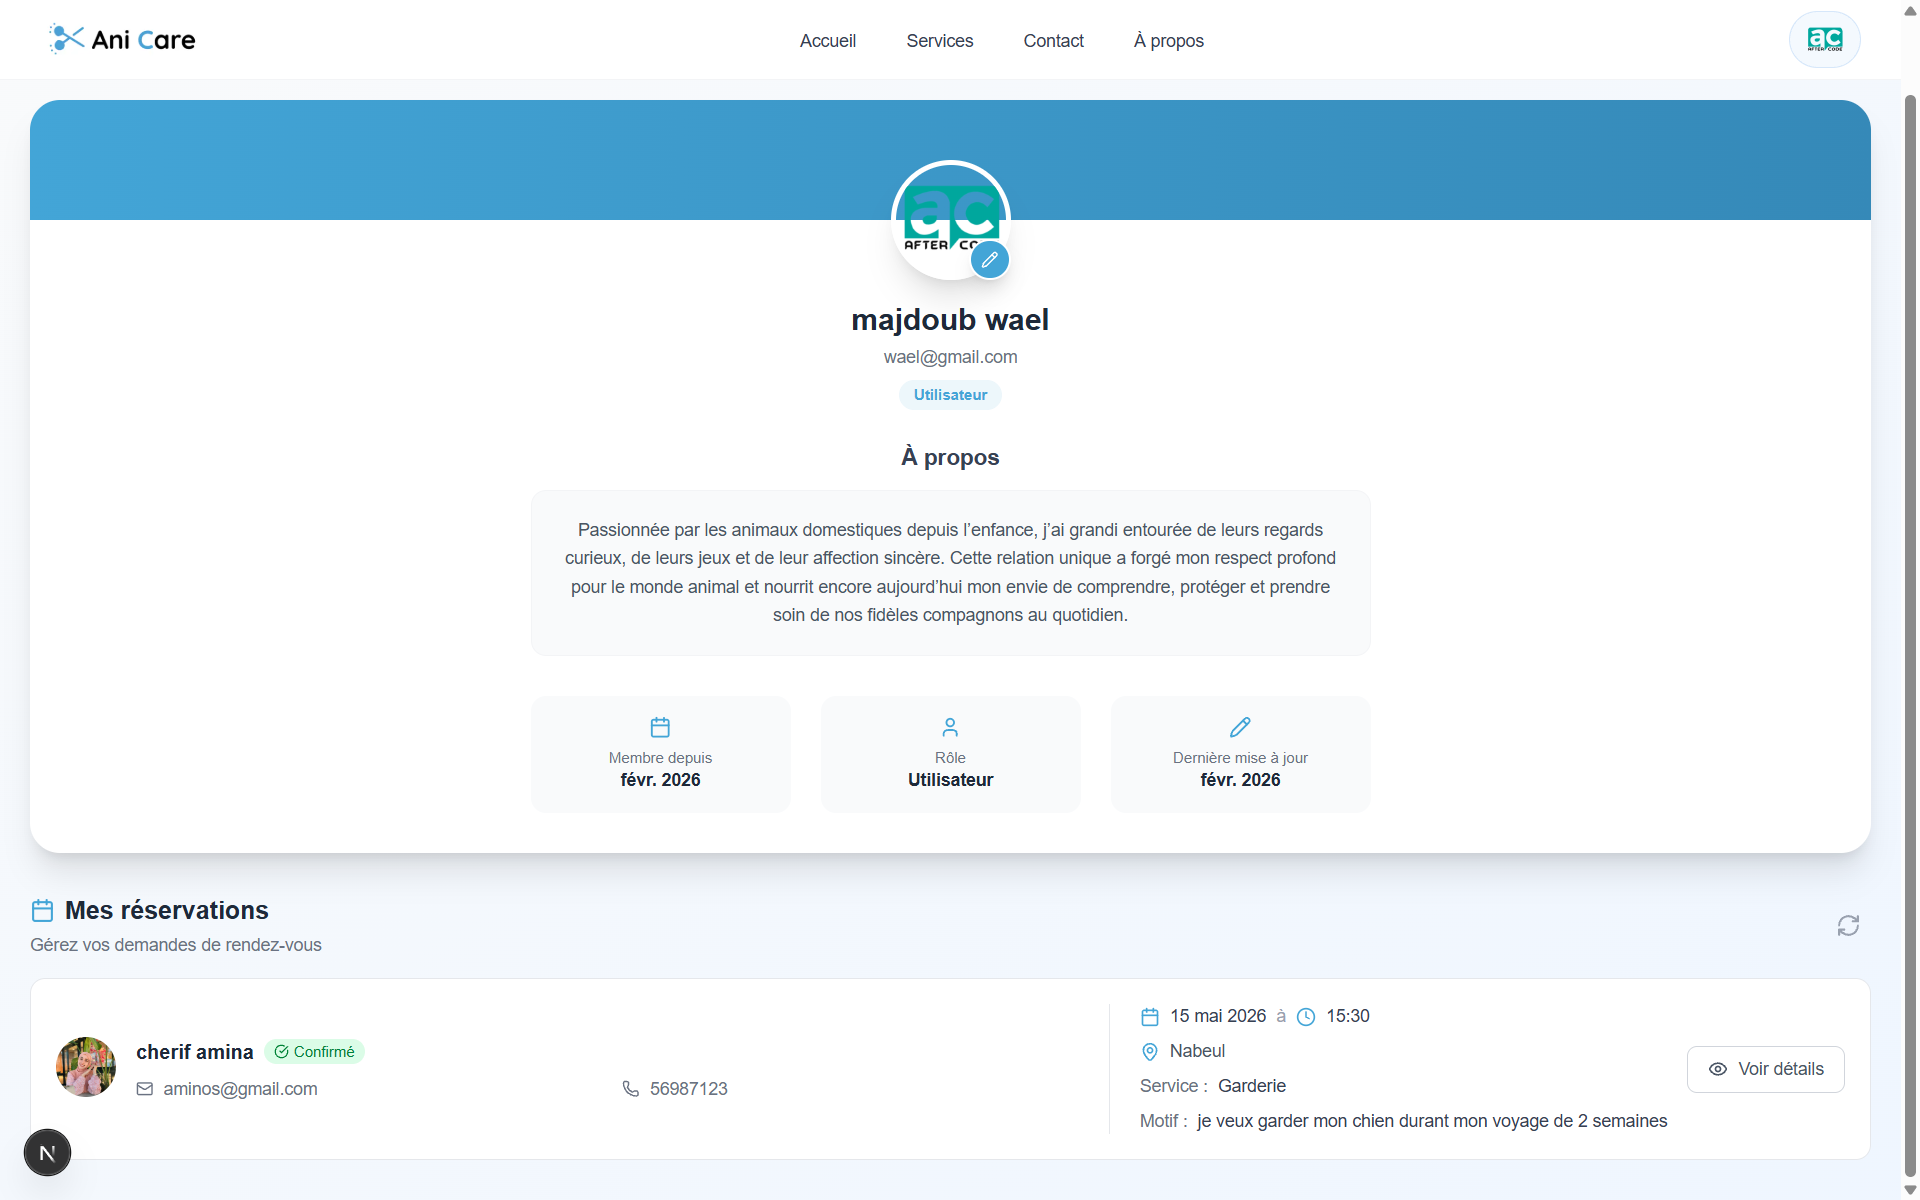
\includegraphics[width=0.73\textwidth]{images/mes reservations.png}
    \caption{Interface de gestion des réservations envoyées pour le demandeur}
\end{figure}   
\subsubsection{Interface des notifications d’acceptation de réservation et de rendez-vous} 
Cette interface illustre les notifications d’acceptation de réservation et de rendez-vous dans le module AniCare : 
\begin{figure}[h!]
    \centering
    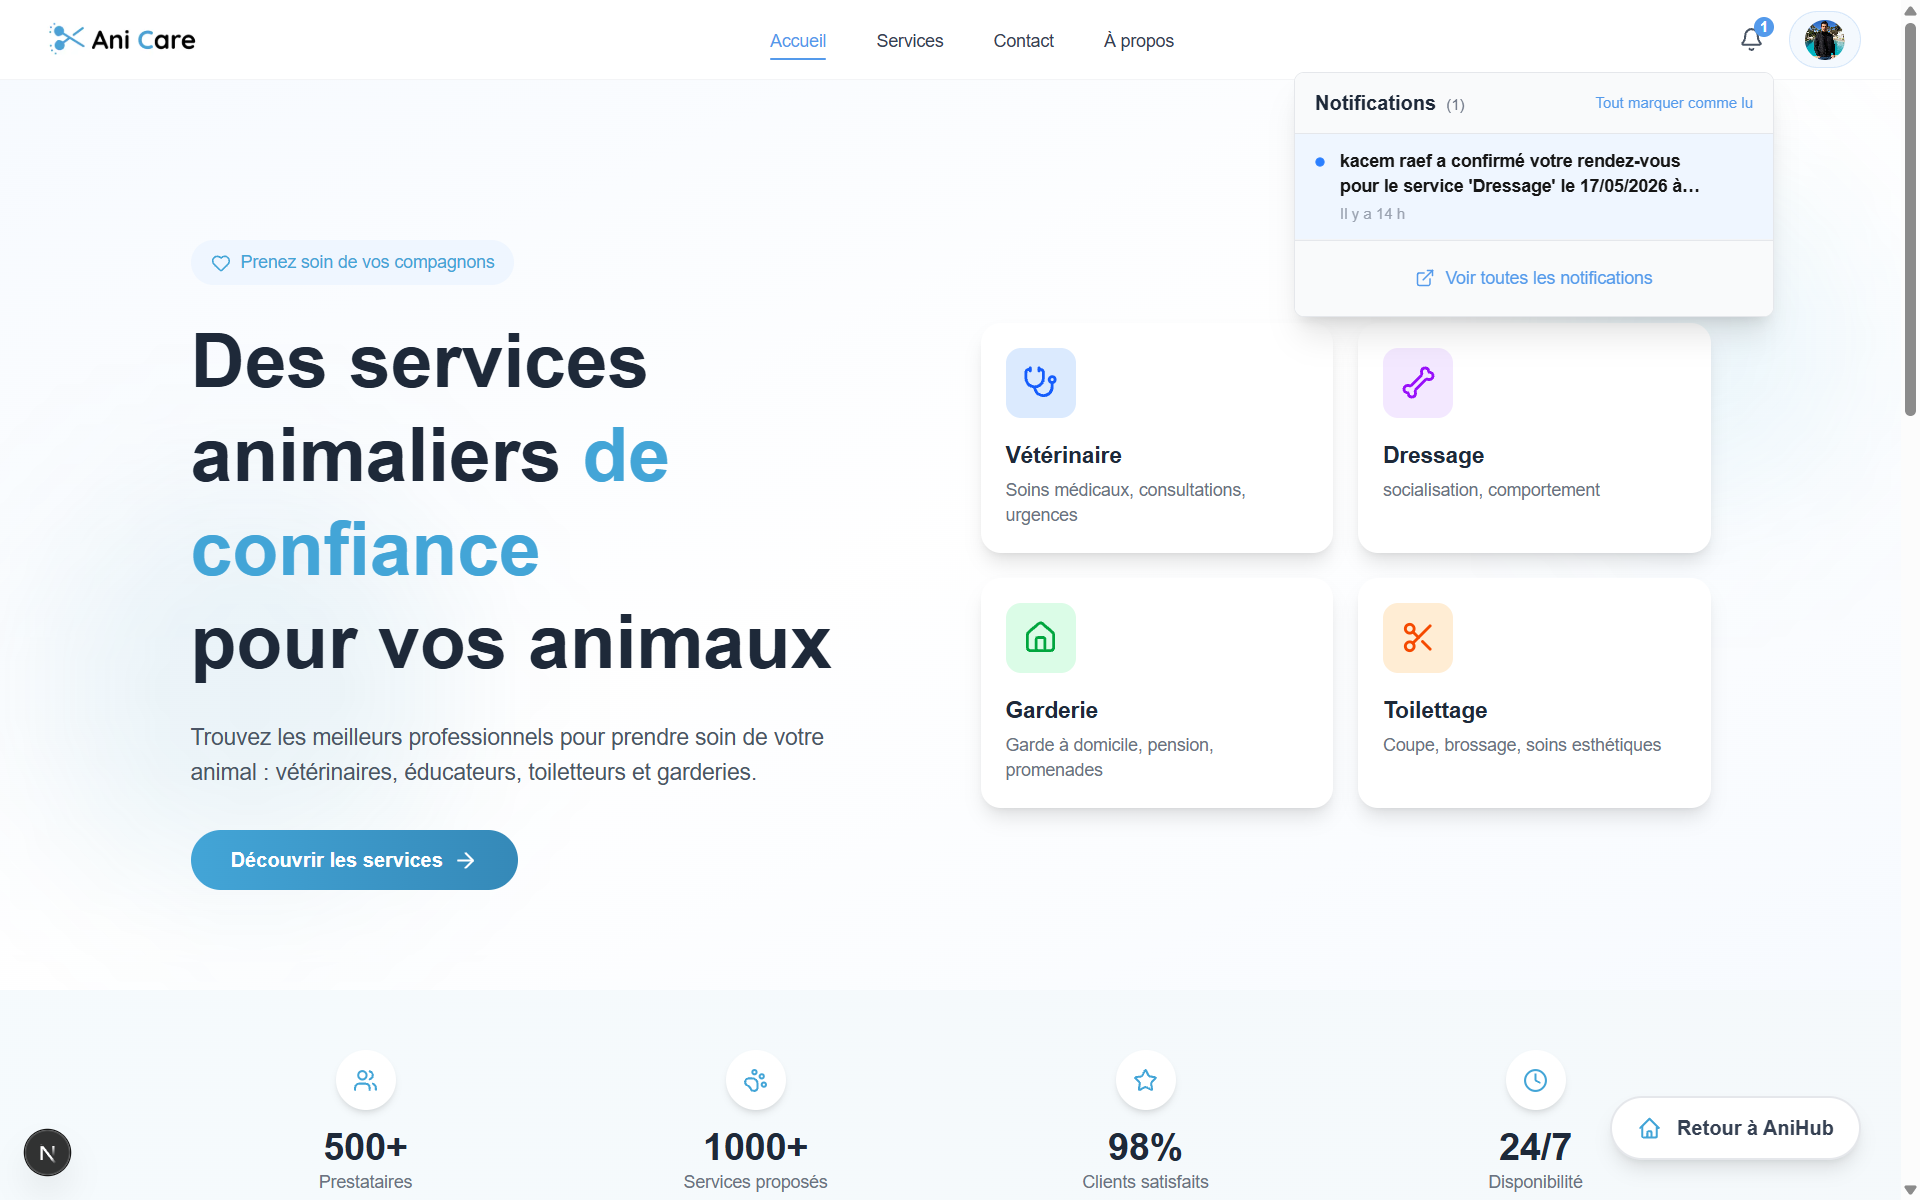
\includegraphics[width=0.73\textwidth]{images/notif anicare.png}
    \caption{Interface des notifications d’acceptation de réservation et de rendez-vous}
\end{figure}   

\newpage
\section{Sprint 6 : Conteneurisation, CI/CD, Déploiement Cloud et Monitoring} 
Dans ce sprint, d’une durée de \textbf{3 semaines}, nous nous sommes concentrés sur la mise en place de l’environnement DevOps de l’application AniHub. Cette étape a permis de conteneuriser les microservices à l’aide de Docker, d’assurer leur orchestration avec Kubernetes et de déployer l’application sur Google Cloud Platform (GCP). Nous avons également mis en œuvre un pipeline CI/CD avec GitHub Actions afin d’automatiser les phases de build et de déploiement. Enfin, un système de monitoring basé sur Grafana et Prometheus a été intégré afin de superviser les performances et la disponibilité des microservices. 
\subsection{Sprint backlog} 
Le tableau suivant présente le Sprint Backlog du sprint 6 avec les user stories, les tâches associées et les efforts estimés : 
\begin{longtable}{|p{1cm}|p{4.7cm}|p{7cm}|p{1.3cm}|}

\caption{Sprint Backlog du sprint 6} \label{tab:sprint6-backlog} \\

\hline
\multicolumn{1}{|c|}{\cellcolor{coloranihub}\textbf{ID}} &
\multicolumn{1}{c|}{\cellcolor{coloranihub}\textbf{User Story}} &
\multicolumn{1}{c|}{\cellcolor{coloranihub}\textbf{Tâches}} &
\multicolumn{1}{c|}{\cellcolor{coloranihub}\textbf{Effort}} \\
\hline
\endfirsthead

\hline
\multicolumn{1}{|c|}{\cellcolor{coloranihub}\textbf{ID}} &
\multicolumn{1}{c|}{\cellcolor{coloranihub}\textbf{User Story}} &
\multicolumn{1}{c|}{\cellcolor{coloranihub}\textbf{Tâches}} &
\multicolumn{1}{c|}{\cellcolor{coloranihub}\textbf{Effort}} \\
\hline
\endhead

% ===================== US61 =====================
\multirow{5}{2cm}{US61}
& \multirow{5}{5cm}{Conteneuriser les microservices avec Docker afin de garantir un environnement d’exécution stable et portable.}
& Création des Dockerfile pour chaque microservice & 1 j \\
\cline{3-4}
& & Build des images Docker & 0.5 j \\
\cline{3-4}
& & Push des images vers Docker Hub & 0.5 j \\
\cline{3-4}
& & Configuration de Docker Compose pour l’environnement local & 0.5 j \\
\cline{3-4}
& & Vérification de l’exécution des conteneurs & 0.5 j \\
\hline

% ===================== US62 =====================
\multirow{5}{2cm}{US62}
& \multirow{5}{5cm}{Déployer les microservices sur Kubernetes afin d’assurer l’orchestration et la disponibilité de l’application.}
& Création des fichiers Deployment et Service Kubernetes & 1 j \\
\cline{3-4}
& & Configuration des pods et replicas & 0.5 j \\
\cline{3-4}
& & Mise en place des Ingress pour l’accès aux services & 0.5 j \\
\cline{3-4}
& & Déploiement sur le cluster Kubernetes & 0.5 j \\
\cline{3-4}
& & Tests de communication entre microservices & 0.5 j \\
\hline

% ===================== US63 =====================
\multirow{4}{2cm}{US63}
& \multirow{4}{5cm}{Déployer l’application sur Google Cloud Platform (GCP) afin de rendre la plateforme accessible en ligne.}
& Création du cluster Kubernetes sur GCP & 1 j \\
\cline{3-4}
& & Configuration de l’environnement cloud & 0.5 j \\
\cline{3-4}
& & Déploiement des microservices sur GCP & 0.5 j \\
\cline{3-4}
& & Validation de l’accès externe & 0.5 j \\
\hline

% ===================== US64 =====================
\multirow{4}{2cm}{US64}
& \multirow{4}{5cm}{Automatiser le build et le déploiement avec GitHub Actions afin d’assurer un processus CI/CD rapide et fiable.}
& Création du workflow GitHub Actions & 0.5 j \\
\cline{3-4}
& & Automatisation du build Docker & 0.5 j \\
\cline{3-4}
& & Pull des images depuis Docker Hub & 0.5 j \\
\cline{3-4}
& & Déploiement automatique sur Kubernetes & 0.5 j \\
\hline

% ===================== US65 =====================
\multirow{4}{2cm}{US65}
& \multirow{4}{5cm}{Surveiller les microservices avec Grafana afin de suivre les performances et détecter les anomalies du système.}
& Installation de Prometheus pour la collecte des métriques & 0.5 j \\
\cline{3-4}
& & Configuration de Grafana & 0.5 j \\
\cline{3-4}
& & Création des dashboards de monitoring & 0.5 j \\
\cline{3-4}
& & Surveillance des pods et ressources Kubernetes & 0.5 j \\
\hline
\end{longtable}  


\subsection{Conteneurisation des microservices avec Docker}  

\subsubsection{Création des fichiers Dockerfile}

Cette figure présente un exemple de Dockerfile du microservice \textit{AniMatch}, utilisé pour définir et automatiser la création d’une image Docker pour ce microservice :   

\begin{figure}[H]
    \centering
    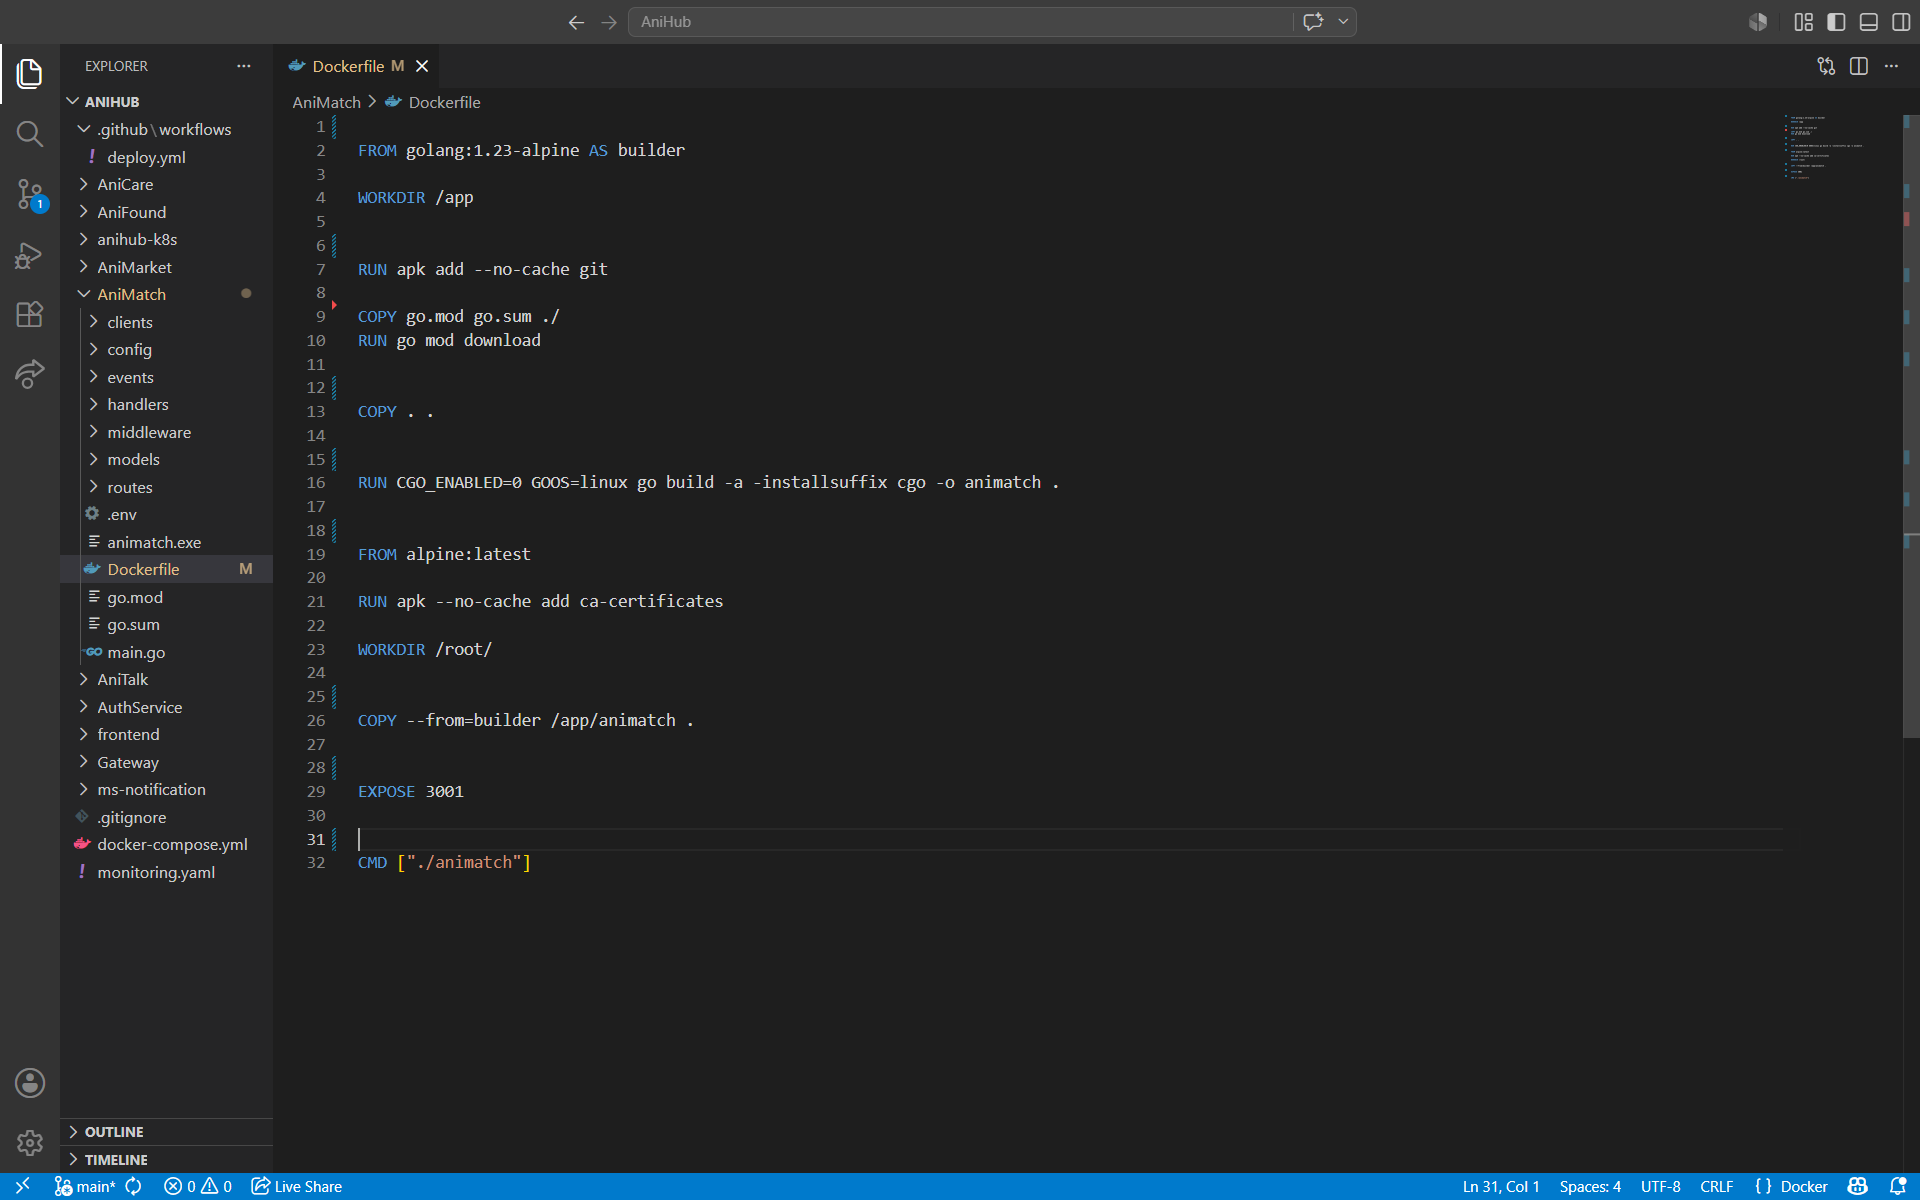
\includegraphics[width=0.65\linewidth]{images/dokcer file.png}
    \caption{Exemple de fichier Dockerfile du microservice \textit{AniMatch}}
    \label{fig:dockerfile-animatch}
\end{figure}

 \newpage
\subsubsection{Configuration de Docker Compose}

Cette figure illustre notre fichier \textit{docker-compose.yml}, utilisé pour orchestrer et exécuter l’ensemble des microservices ainsi que leurs dépendances dans des conteneurs Docker : 

\begin{figure}[H]
    \centering
    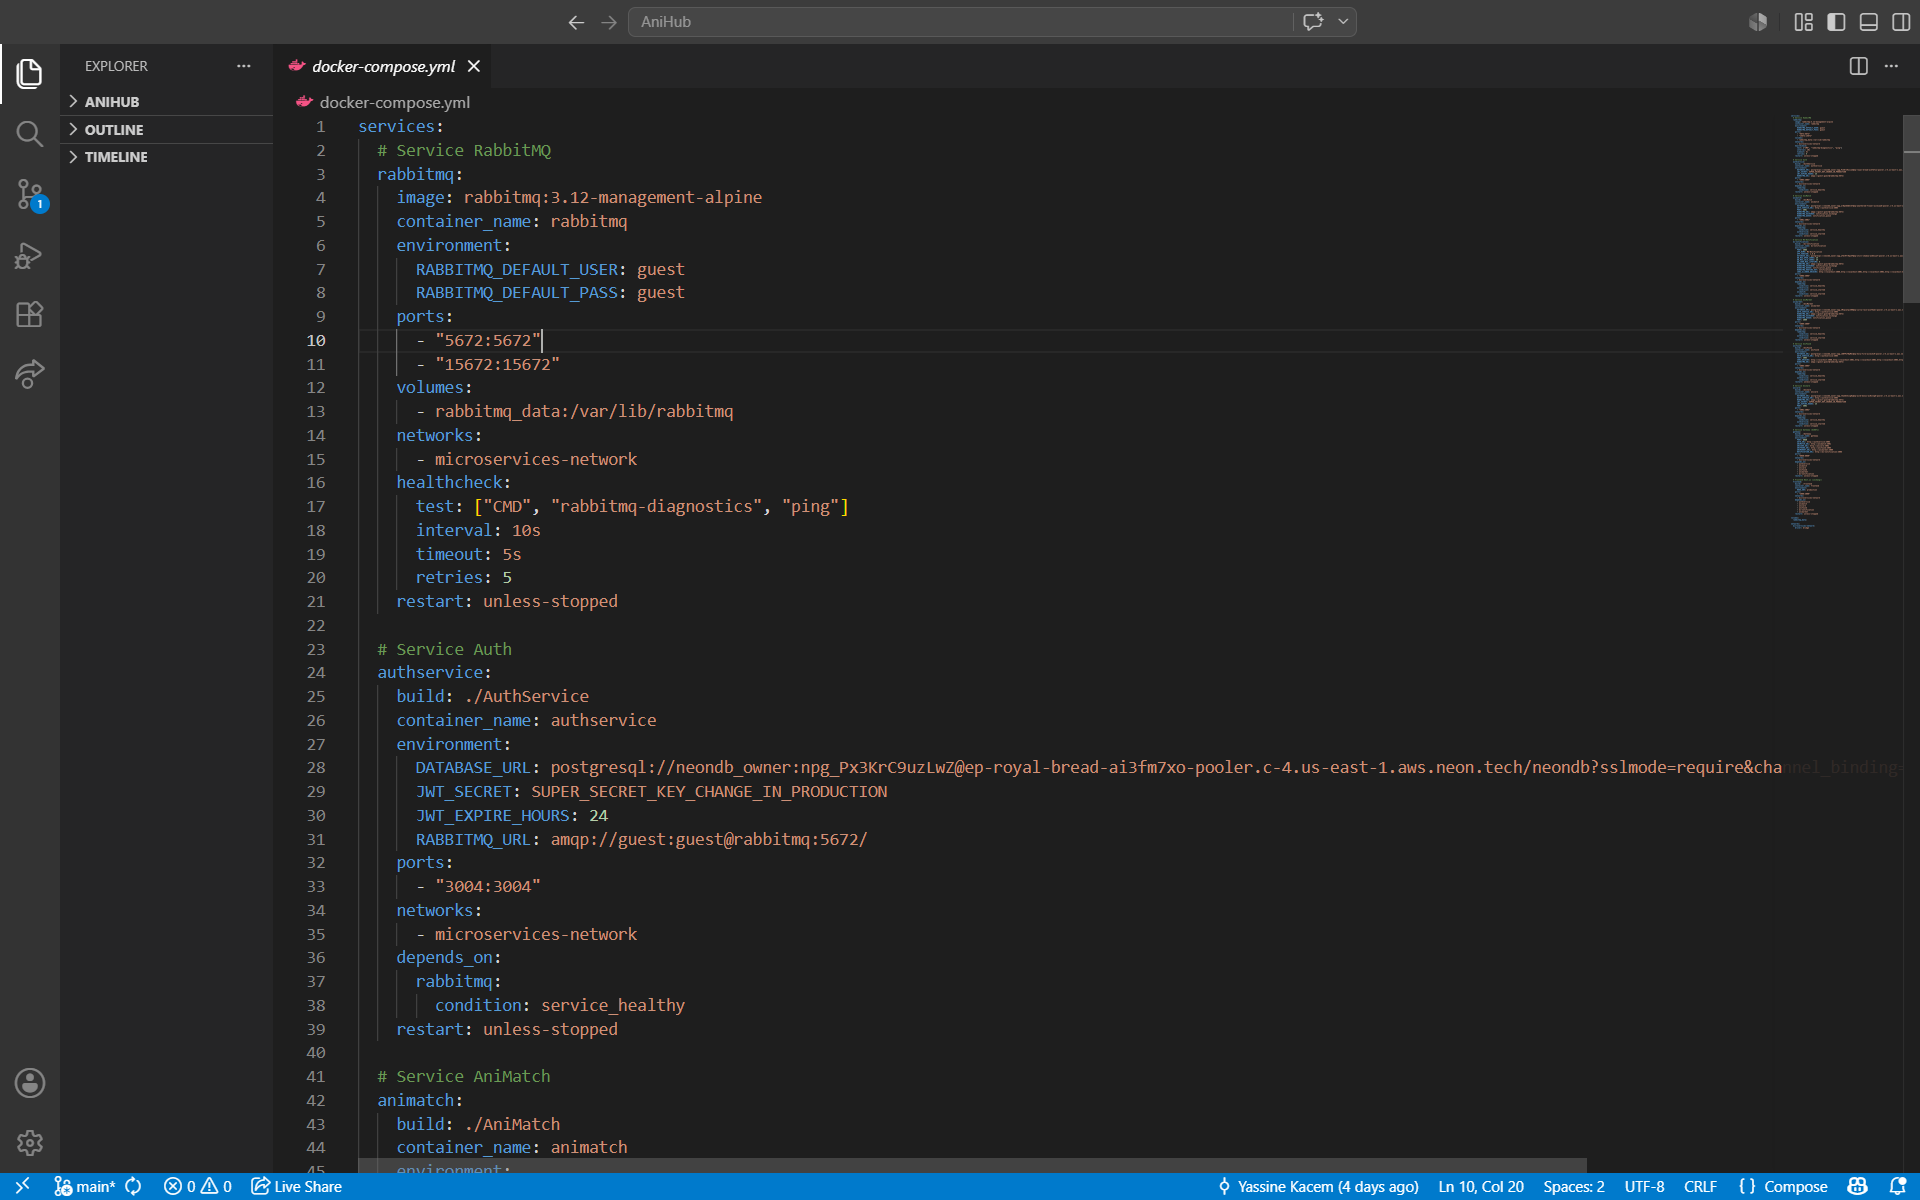
\includegraphics[width=0.75\linewidth]{images/docker compose.png}
    \caption{Configuration du fichier Docker Compose}
    \label{fig:docker-compose}
\end{figure}  
\subsubsection{Construction et exécution des conteneurs} 
Ces figures présentent les différentes étapes de construction et de lancement des conteneurs de l’application.
\begin{figure}[h!]
    \centering
    
    \begin{minipage}{0.48\textwidth}
        \centering
        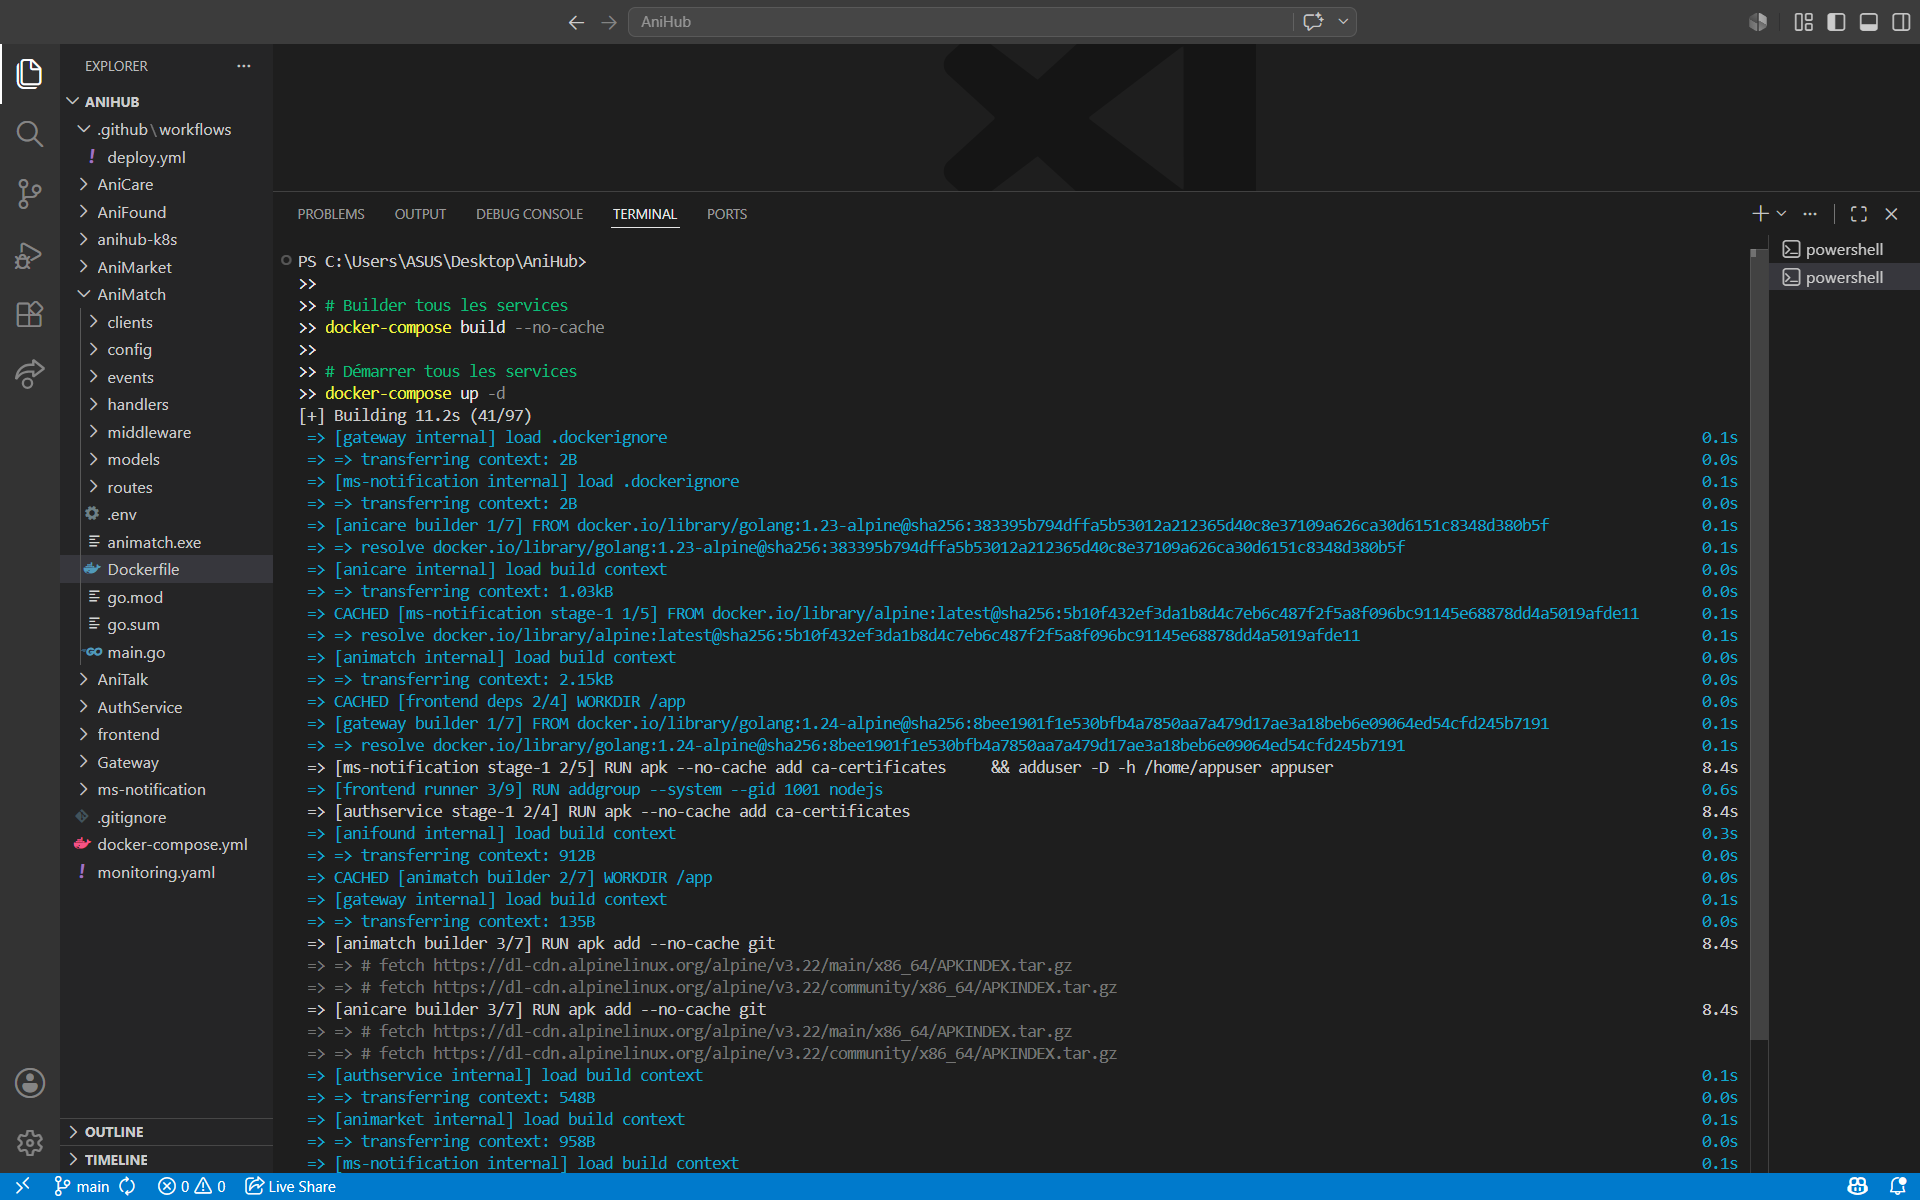
\includegraphics[width=\textwidth,height=5.6cm]{images/creation des conteneurs.png}
        \caption{Construction et démarrage des conteneurs}
    \end{minipage}
    \hfill
    \begin{minipage}{0.48\textwidth}
        \centering
        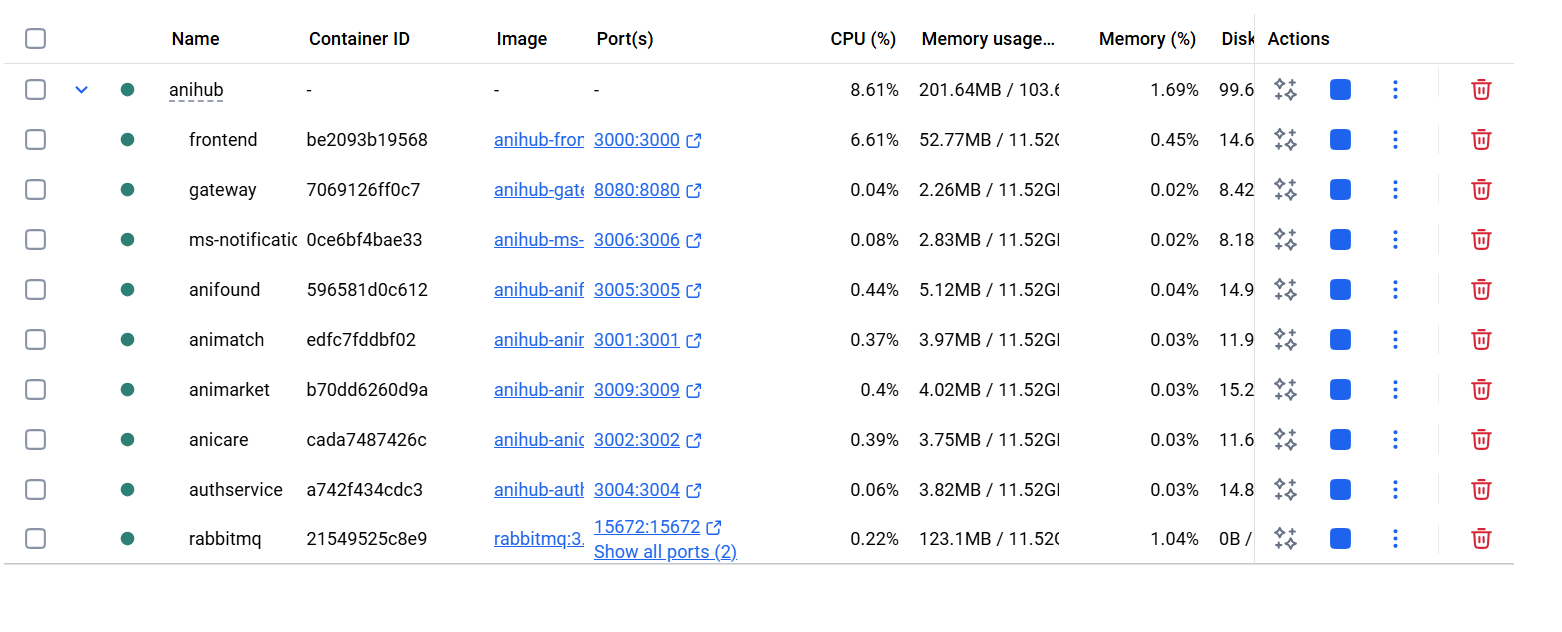
\includegraphics[width=\textwidth,height=5.6cm]{images/execution des conteneurs.png}
        \caption{Conteneurs Docker en cours d’exécution}
    \end{minipage}

\end{figure}
 \newpage
\subsection{Déploiement des microservices avec Kubernetes}  
\subsubsection{Création des fichiers Deployment et Service}

Cette figure illustre le fichier \textit{deployment-anifound.yaml}, utilisé pour définir et déployer le microservice \textit{AniFound} dans l’environnement Kubernetes.

\begin{figure}[H]
    \centering
    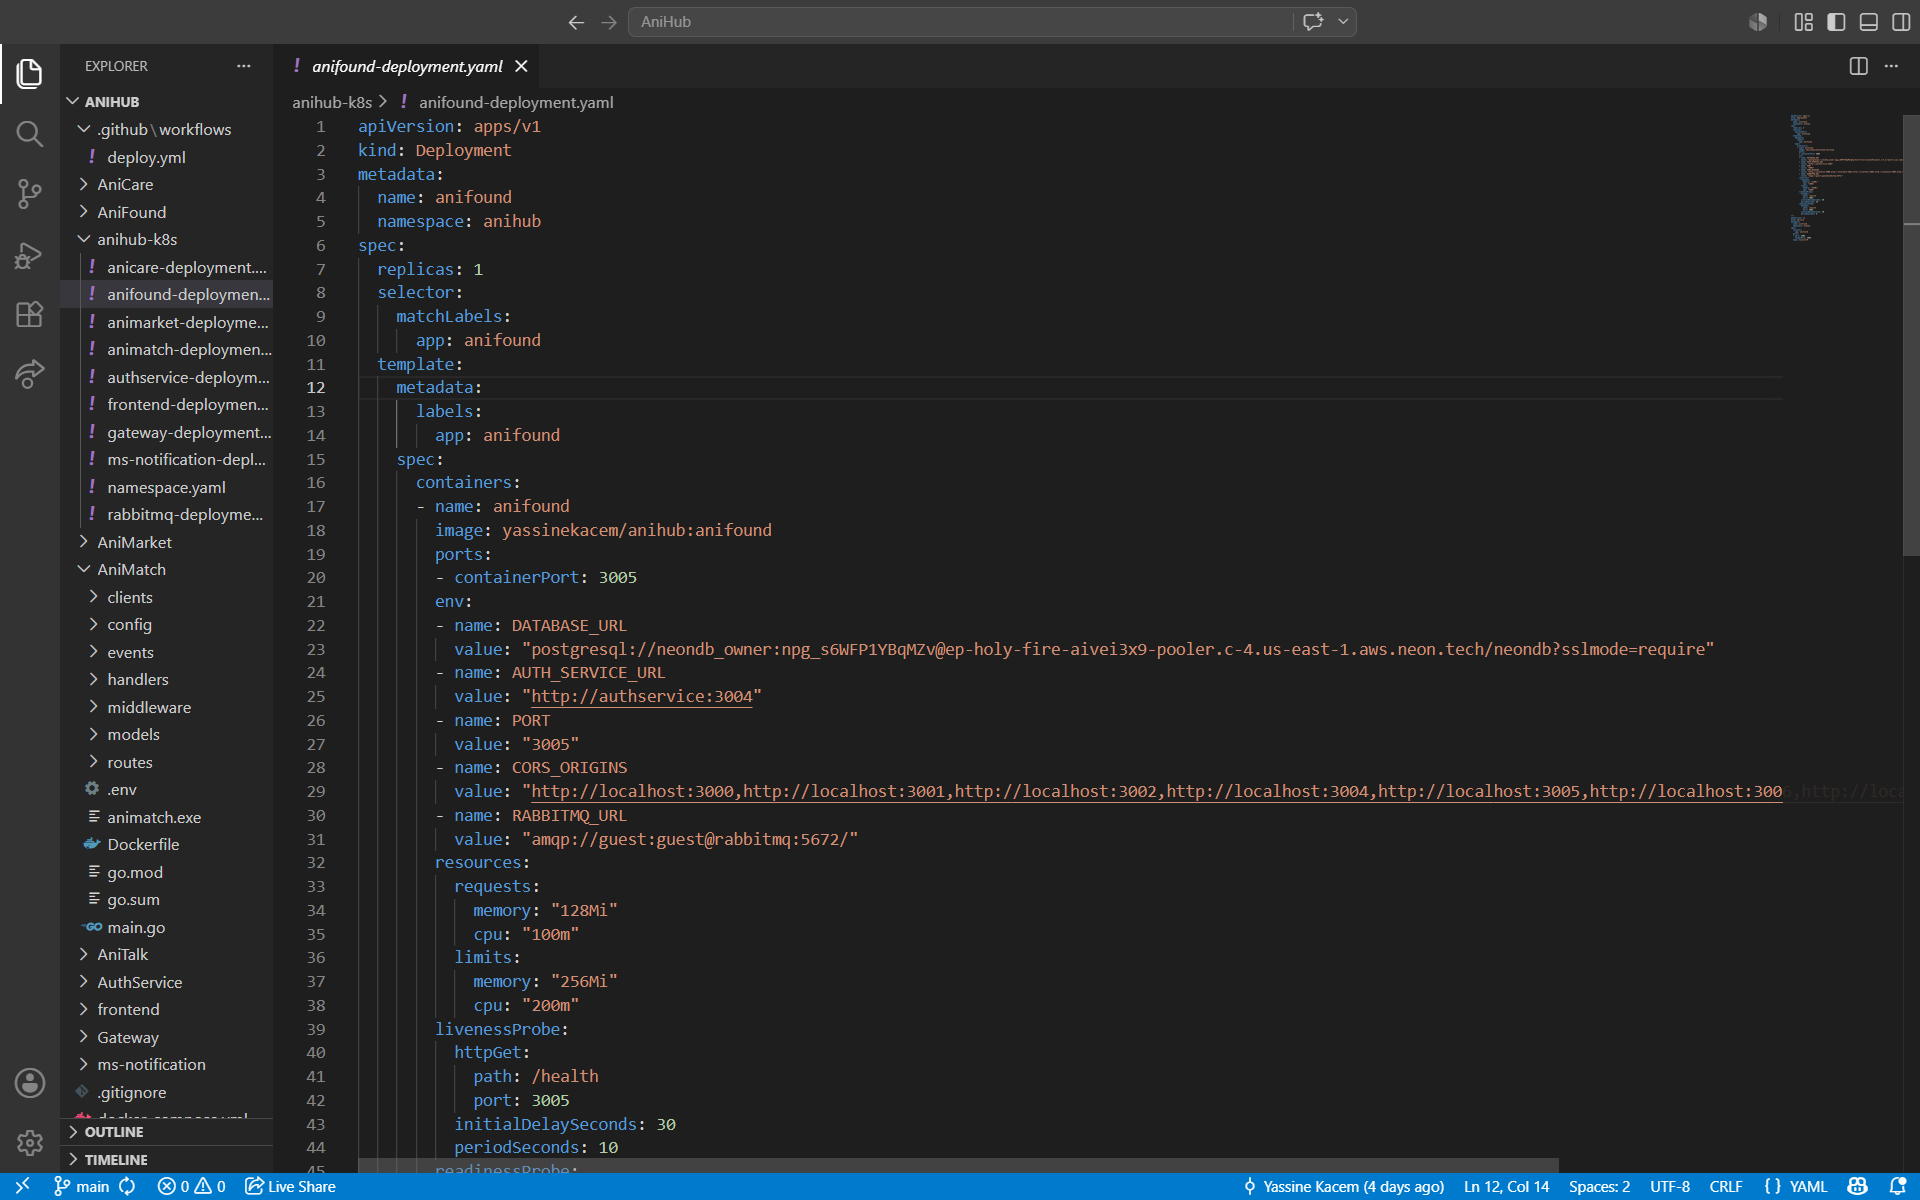
\includegraphics[width=0.7\linewidth]{images/deploymentservice k8s.png}
    \caption{Fichier Deployment du microservice \textit{AniFound}}
    \label{fig:deployment-anifound}
\end{figure}   

\subsubsection{Application des fichiers YAML dans Kubernetes pour le déploiement d’AniHub} 
Cette figure illustre l’application des fichiers de configuration YAML dans Kubernetes pour déployer les microservices d’AniHub : 
\begin{figure}[H]
    \centering
    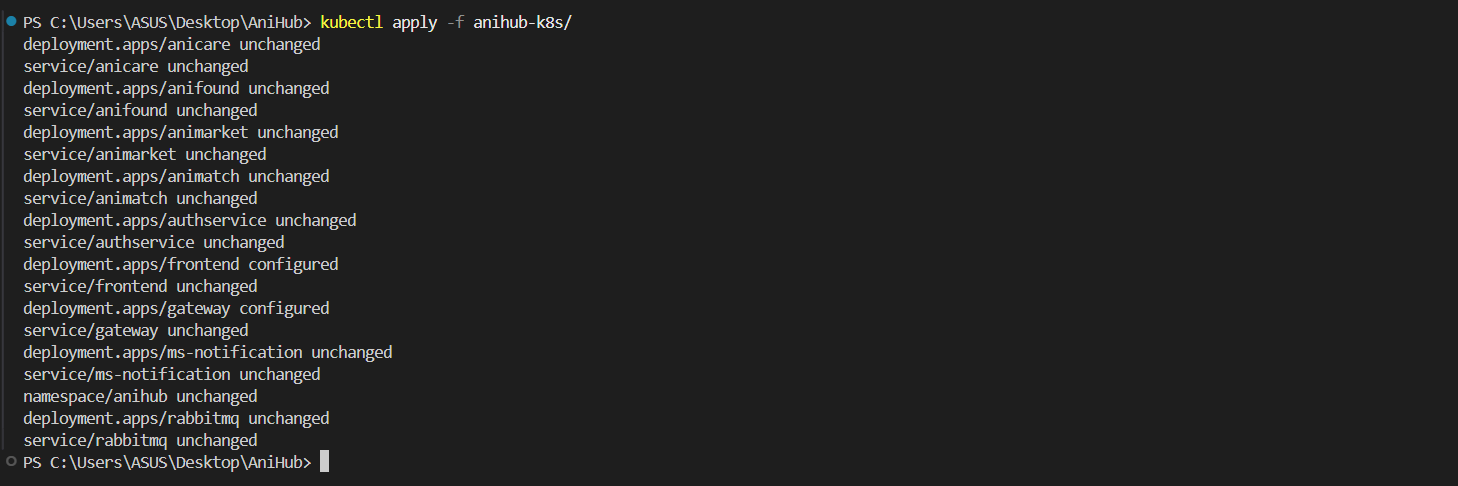
\includegraphics[width=0.9\linewidth]{images/apply files k8s.png}
    \caption{Application des fichiers YAML dans Kubernetes pour le déploiement d’AniHub}
    \label{fig:deploiement-k8s} 
\end{figure}
\newpage 
\subsubsection{Vérification de l’état des pods}  

Cette figure illustre l’état des pods déployés sur Kubernetes afin de vérifier le bon fonctionnement des différents microservices de l’application AniHub : 
\begin{figure}[H]
    \centering
    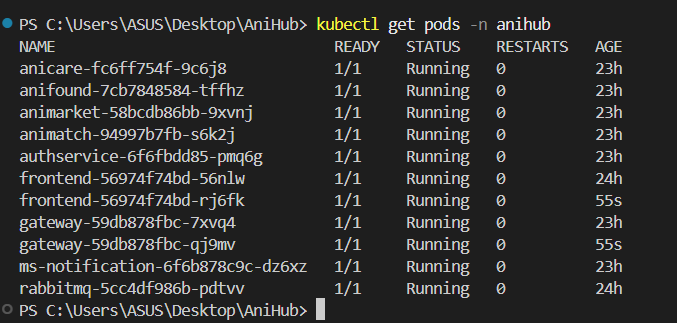
\includegraphics[width=0.56\linewidth]{images/get pods.png}
    \caption{Vérification de l’état des pods sur Kubernetes}
    \label{fig:pods-k8s}
\end{figure} 

\subsubsection{Exécution des conteneurs via Kubernetes}

Cette figure illustre l’exécution des conteneurs de l’application AniHub dans Docker Desktop, orchestrés par Kubernetes avec un nombre de replicas égal à 1 pour chaque microservice : 
\begin{figure}[H]
    \centering
    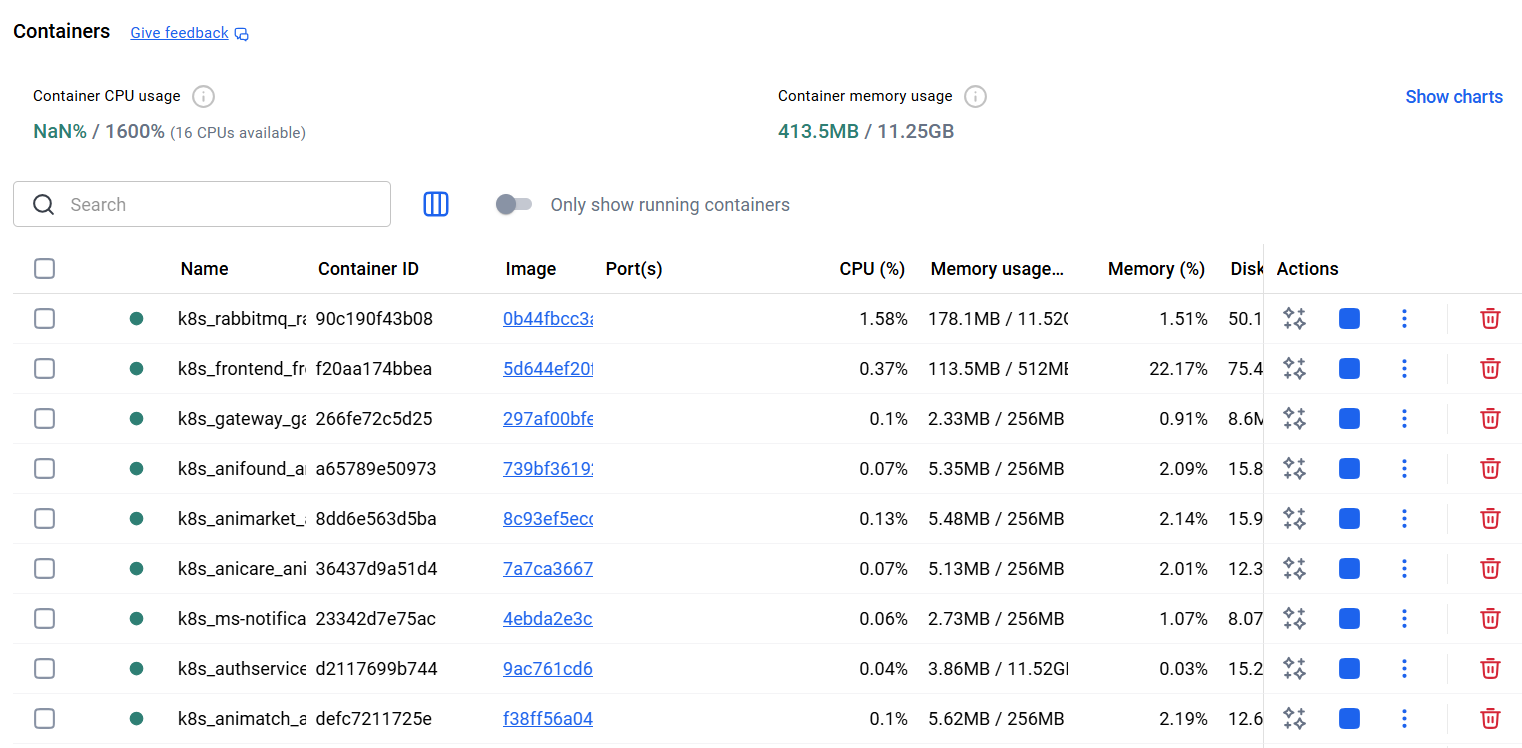
\includegraphics[width=0.56\linewidth]{images/conatiner run from k8s.png}
    \caption{Exécution des conteneurs de l’application AniHub via Kubernetes}
    \label{fig:containers-k8s}
\end{figure} 
\subsubsection{Accès au frontend via port-forward sur le port 3000}
Cette figure illustre l’accès à l’interface frontend de l’application AniHub via un port-forward Kubernetes sur le port 3000, afin de tester l’application en local après le déploiement : 
\begin{figure}[H]
    \centering
    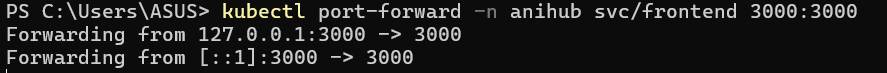
\includegraphics[width=0.66\linewidth]{images/forward.png}
    \caption{Accès au frontend via port-forward sur le port 3000}
    \label{fig:port-forward}
\end{figure} 
\newpage
\subsection{Déploiement Cloud sur Google Cloud Platform} 


\subsubsection{Vérification du contexte cloud}

Cette étape consiste à vérifier que le contexte Kubernetes est bien configuré sur le cluster cloud d’AniHub. Elle permet de s’assurer que les commandes kubectl sont exécutées sur le bon cluster GCP et que l’environnement cible est correctement sélectionné avant le déploiement ou les tests : 

\begin{figure}[H]
    \centering
    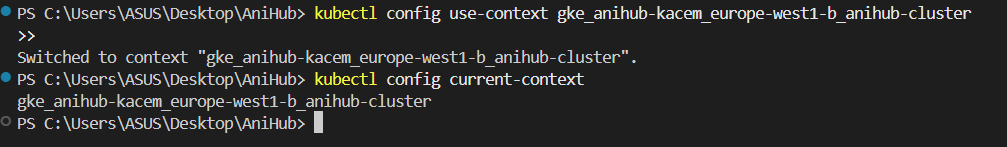
\includegraphics[width=0.76\linewidth]{images/verifons context cloud 1.png}
    \caption{Vérification du contexte Kubernetes sur le cluster cloud de GCP}
    \label{fig:context-cloud}
\end{figure} 

\subsubsection{Affichage des clusters disponibles sur GCP}
Cette figure illustre la liste des clusters Kubernetes disponibles sur Google Cloud Platform (GCP) afin de confirmer que le cluster destiné au déploiement d’AniHub est bien présent et accessible : 
\begin{figure}[H]
    \centering
    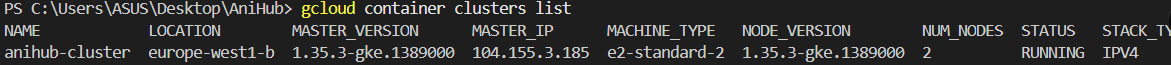
\includegraphics[width=0.96\linewidth]{images/Voir les clusters GCP disponibles 2.png}
    \caption{Affichage des clusters Kubernetes disponibles sur GCP}
    \label{fig:clusters-gcp}
\end{figure}  

\subsubsection{État des pods dans le cluster AniHub sur GCP} 
Cette figure illustre l’état des pods déployés dans le cluster Kubernetes d’AniHub sur Google Cloud Platform (GCP) afin de vérifier que les microservices sont correctement déployés et en cours d’exécution : 
\begin{figure}[H]
    \centering
    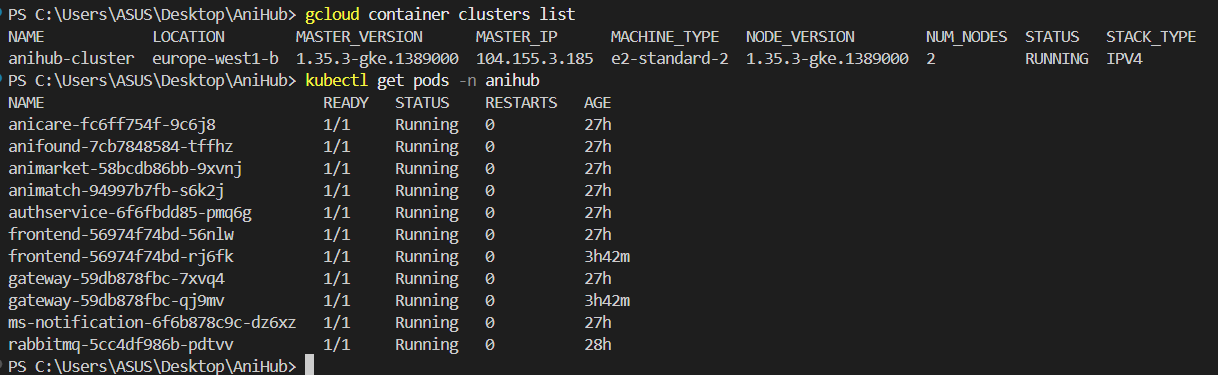
\includegraphics[width=0.76\linewidth]{images/etat des pods dans le cluster.png}
    \caption{État des pods dans le cluster AniHub sur GCP}
    \label{fig:pods-gcp}
\end{figure} 

\newpage  
\subsubsection{Accès cloud et tests de communication entre les microservices } 
Cette figure illustre l’accès à l’application déployée sur le cloud ainsi que les tests de communication entre les microservices frontend et authservice : 
\begin{figure}[H]
    \centering
    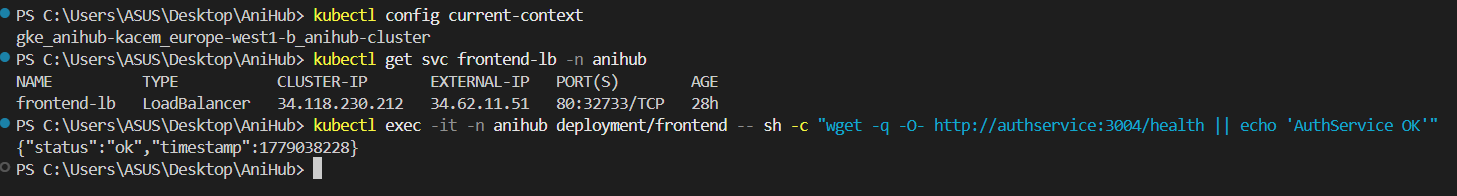
\includegraphics[width=0.76\linewidth]{images/Accès cloud et tests de communication entre microservices.png}
    \caption{Accès cloud et tests de communication entre les microservices}
    \label{fig:communication-microservices}
\end{figure}

\subsubsection{Liste des services Kubernetes et accès à l’application via l’IP externe} 
Cette figure illustre la liste des services Kubernetes ainsi que l’accès à l’application déployée sur le cloud via l’IP externe : 
\begin{figure}[H]
    \centering
    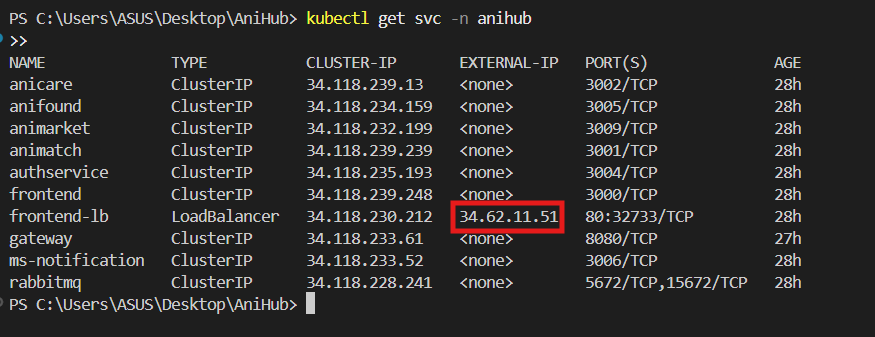
\includegraphics[width=0.62\linewidth]{images/Liste des services Kubernetes et accès à l’application via l’IP externe 4.png}
    \caption{Liste des services Kubernetes et accès à l’application via l’IP externe}
    \label{fig:services-k8s}
\end{figure} 

\subsubsection{Test de l’application déployée via l’IP externe 34.62.11.51 sur le navigateur} 
Cette figure illustre le test de l’application AniHub déployée sur le cloud via l’IP externe : 
\begin{figure}[H]
    \centering
    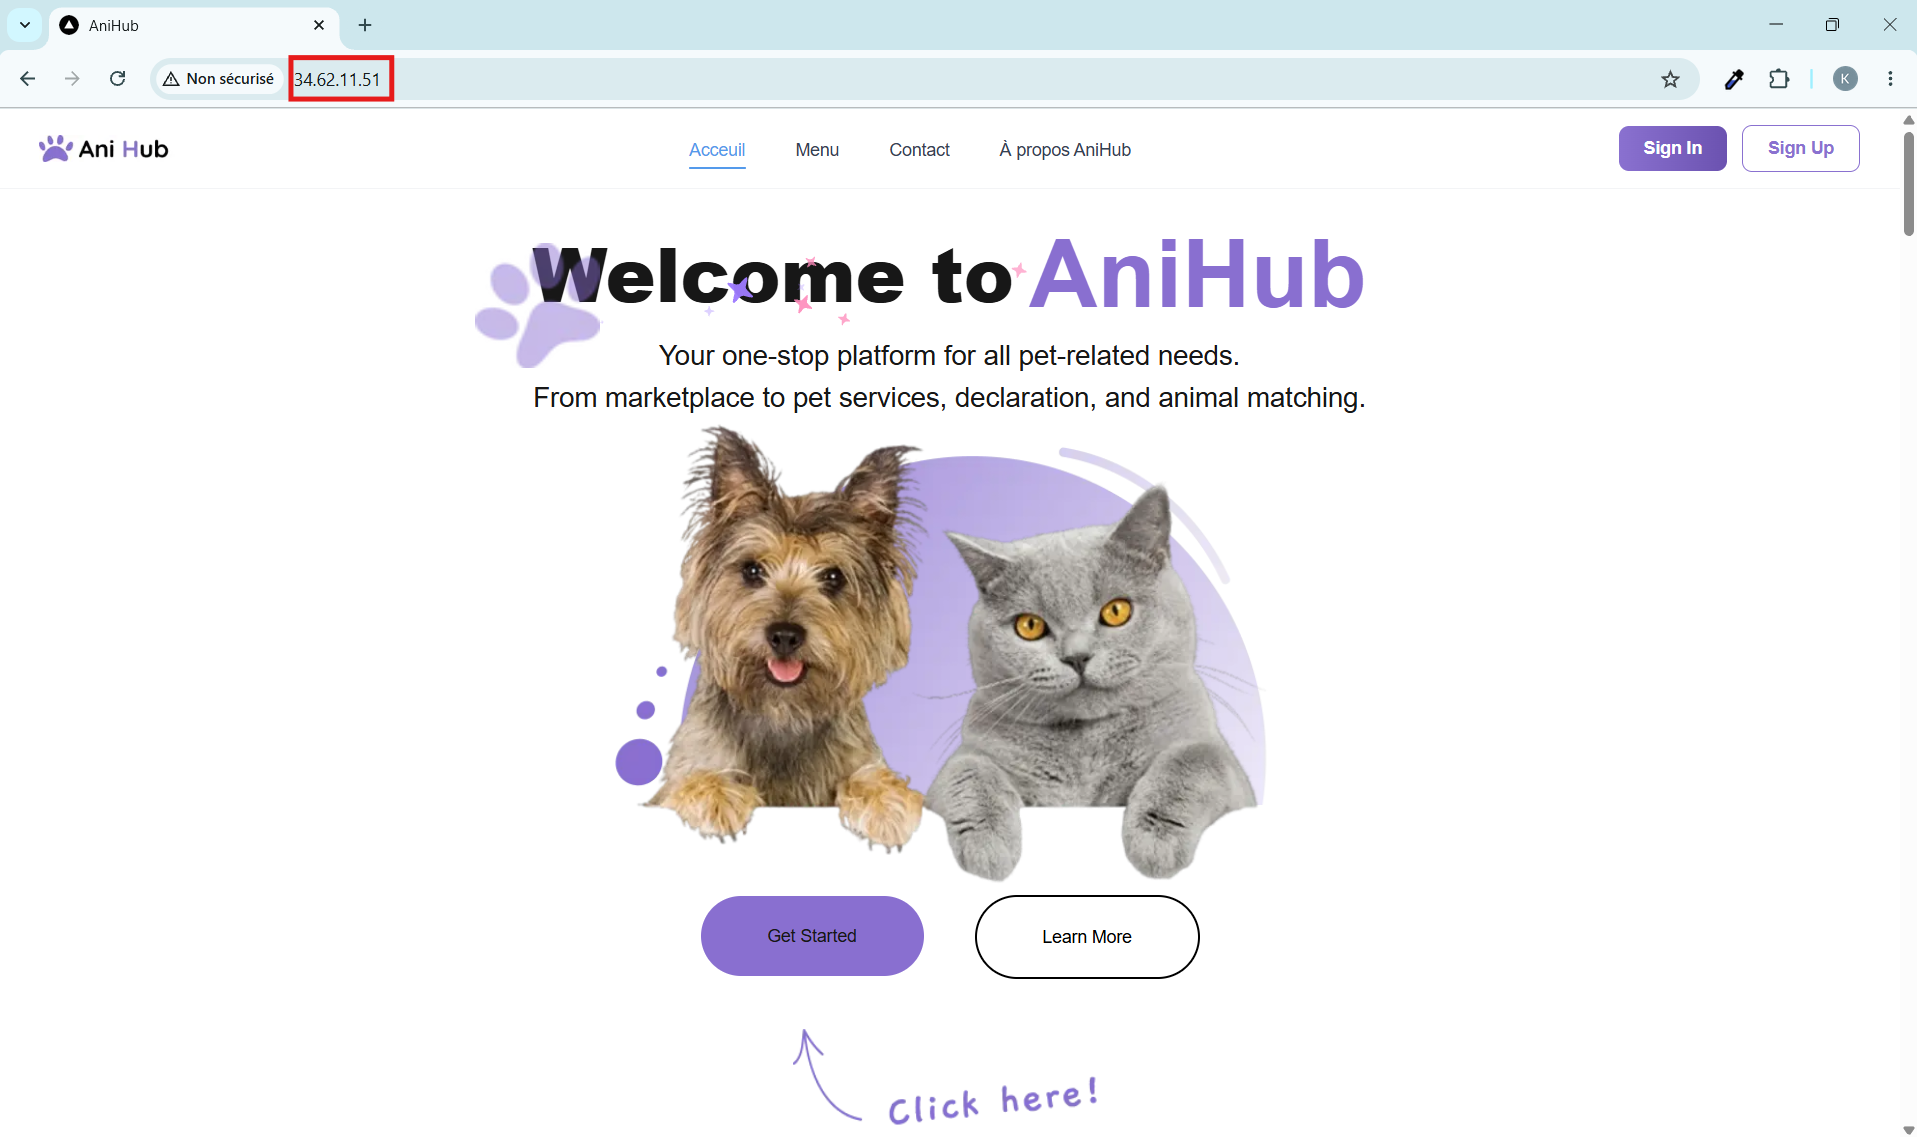
\includegraphics[width=0.72\linewidth]{images/app deployé sur cloud 6.png}
    \caption{Test de l’application déployée via l’IP externe sur le navigateur}
    \label{fig:test-application-cloud}
\end{figure} 
\newpage

\subsection{Mise en place du pipeline CI/CD} 
\subsubsection{Création du workflow GitHub Actions}

Cette figure illustre le fichier \textbf{.github/workflow/deploy.yml} qui définit les étapes nécessaires de la pipeline CI/CD, à savoir :

\begin{itemize}
    \item Authentification à Docker Hub
    \item Construction des images Docker des microservices
    \item Scan et validation des images Docker
    \item Publication des images sur Docker Hub
    \item Authentification à Google Cloud Platform (GCP)
    \item Configuration du SDK Google Cloud
    \item Récupération des identifiants du cluster Kubernetes (GKE)
    \item Déploiement des microservices sur Kubernetes
    \item Redémarrage des déploiements Kubernetes
    \item Attente de la disponibilité des services
    \item Vérification du statut du déploiement
\end{itemize}  

\begin{figure}[H]
    \centering
    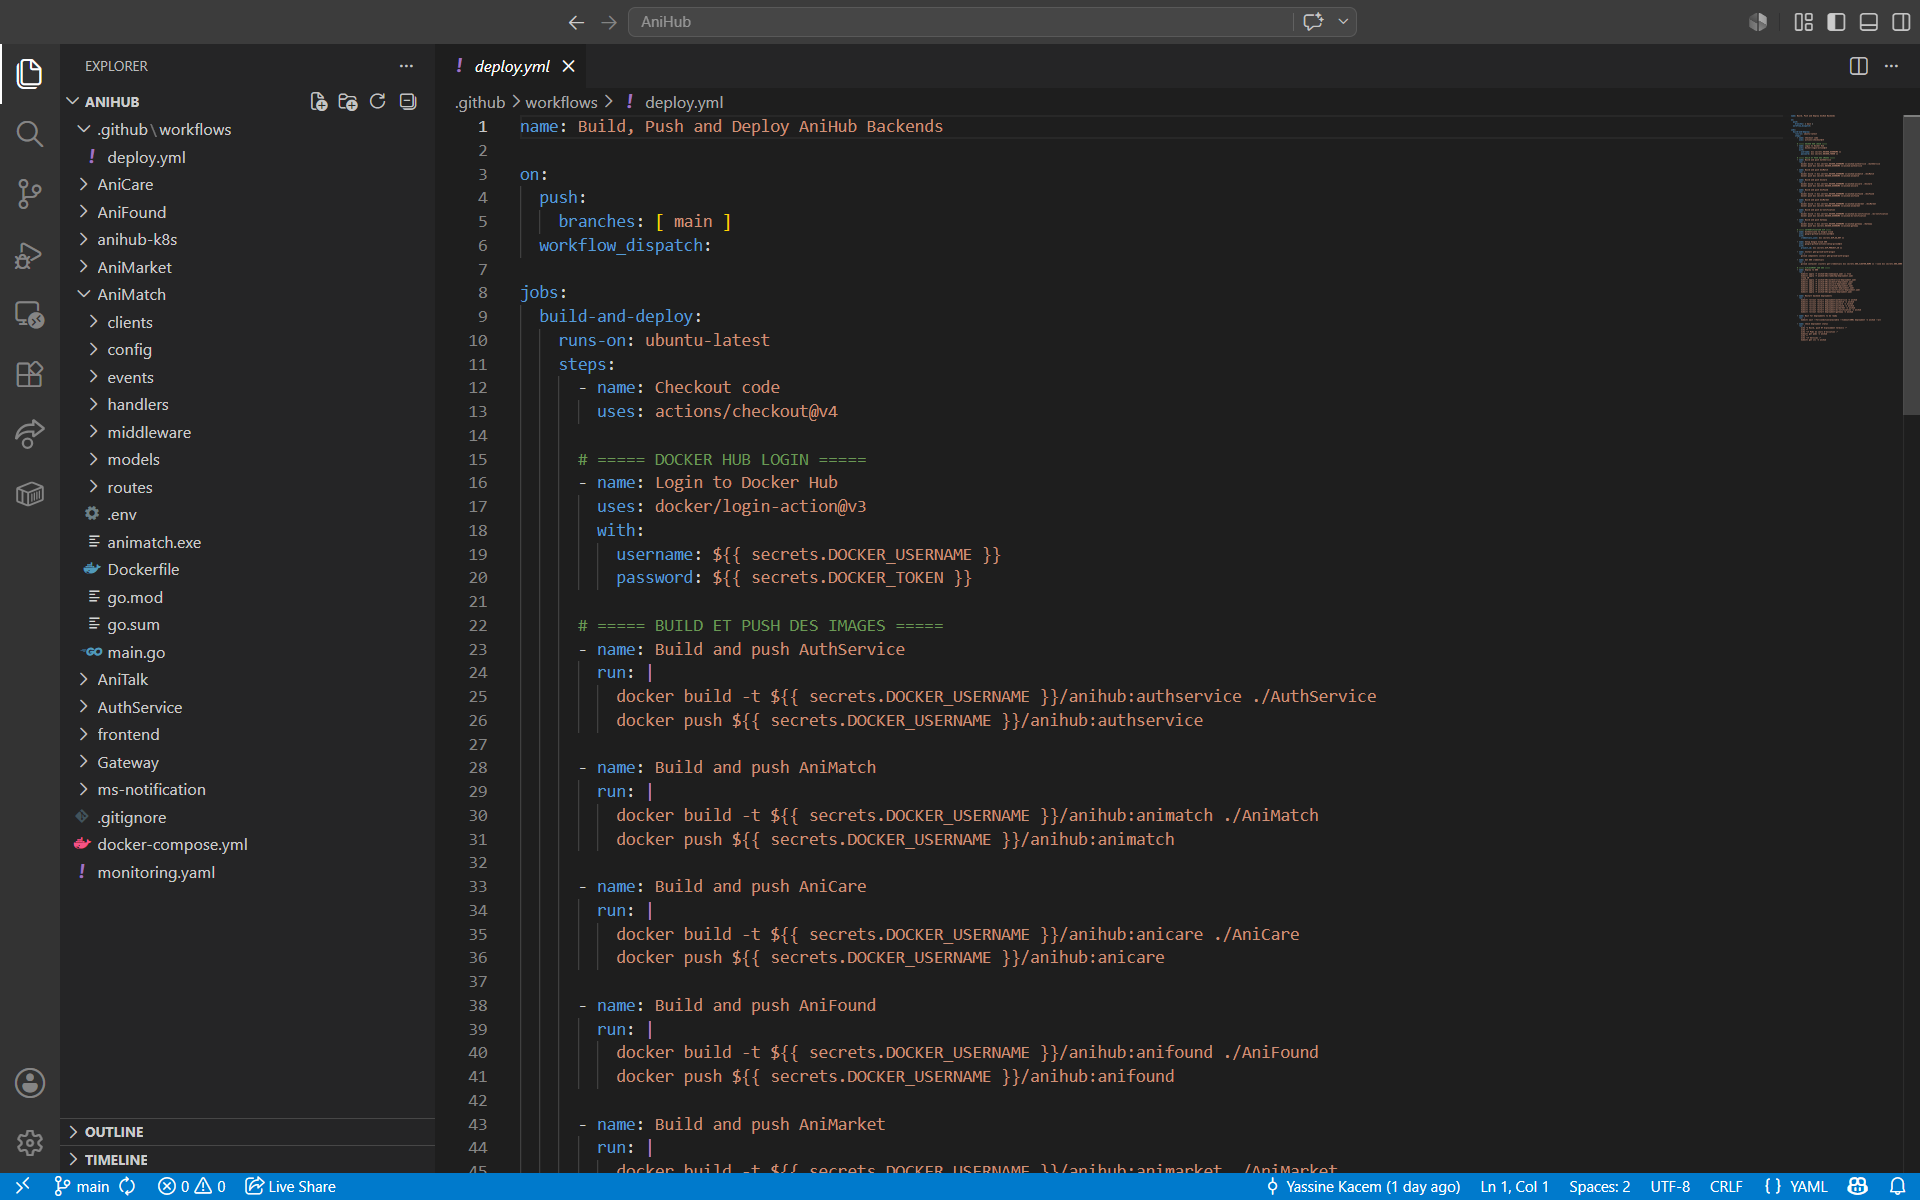
\includegraphics[width=0.68\linewidth]{images/pipeline1.png}
    \caption{Fichier de workflow GitHub Actions pour la pipeline CI/CD}
    \label{fig:workflow-ci-cd}
\end{figure}

\subsubsection{Déclenchement de la pipeline CI/CD par un push sur GitHub} 
Cette figure illustre un push vers le dépôt GitHub permettant de déclencher automatiquement la pipeline CI/CD : 
\begin{figure}[H]
    \centering
    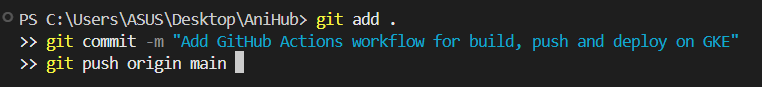
\includegraphics[width=0.55\linewidth]{images/declenche pipeline.png}
    \caption{Déclenchement de la pipeline CI/CD par un push sur GitHub}
    \label{fig:trigger-ci-cd} 
\end{figure}    

\newpage
\subsubsection{Exécution de la pipeline dans GitHub Actions} 
Cette figure illustre l’exécution de la pipeline CI/CD dans GitHub Actions après un push sur le dépôt GitHub : 
\begin{figure}[H]
    \centering
    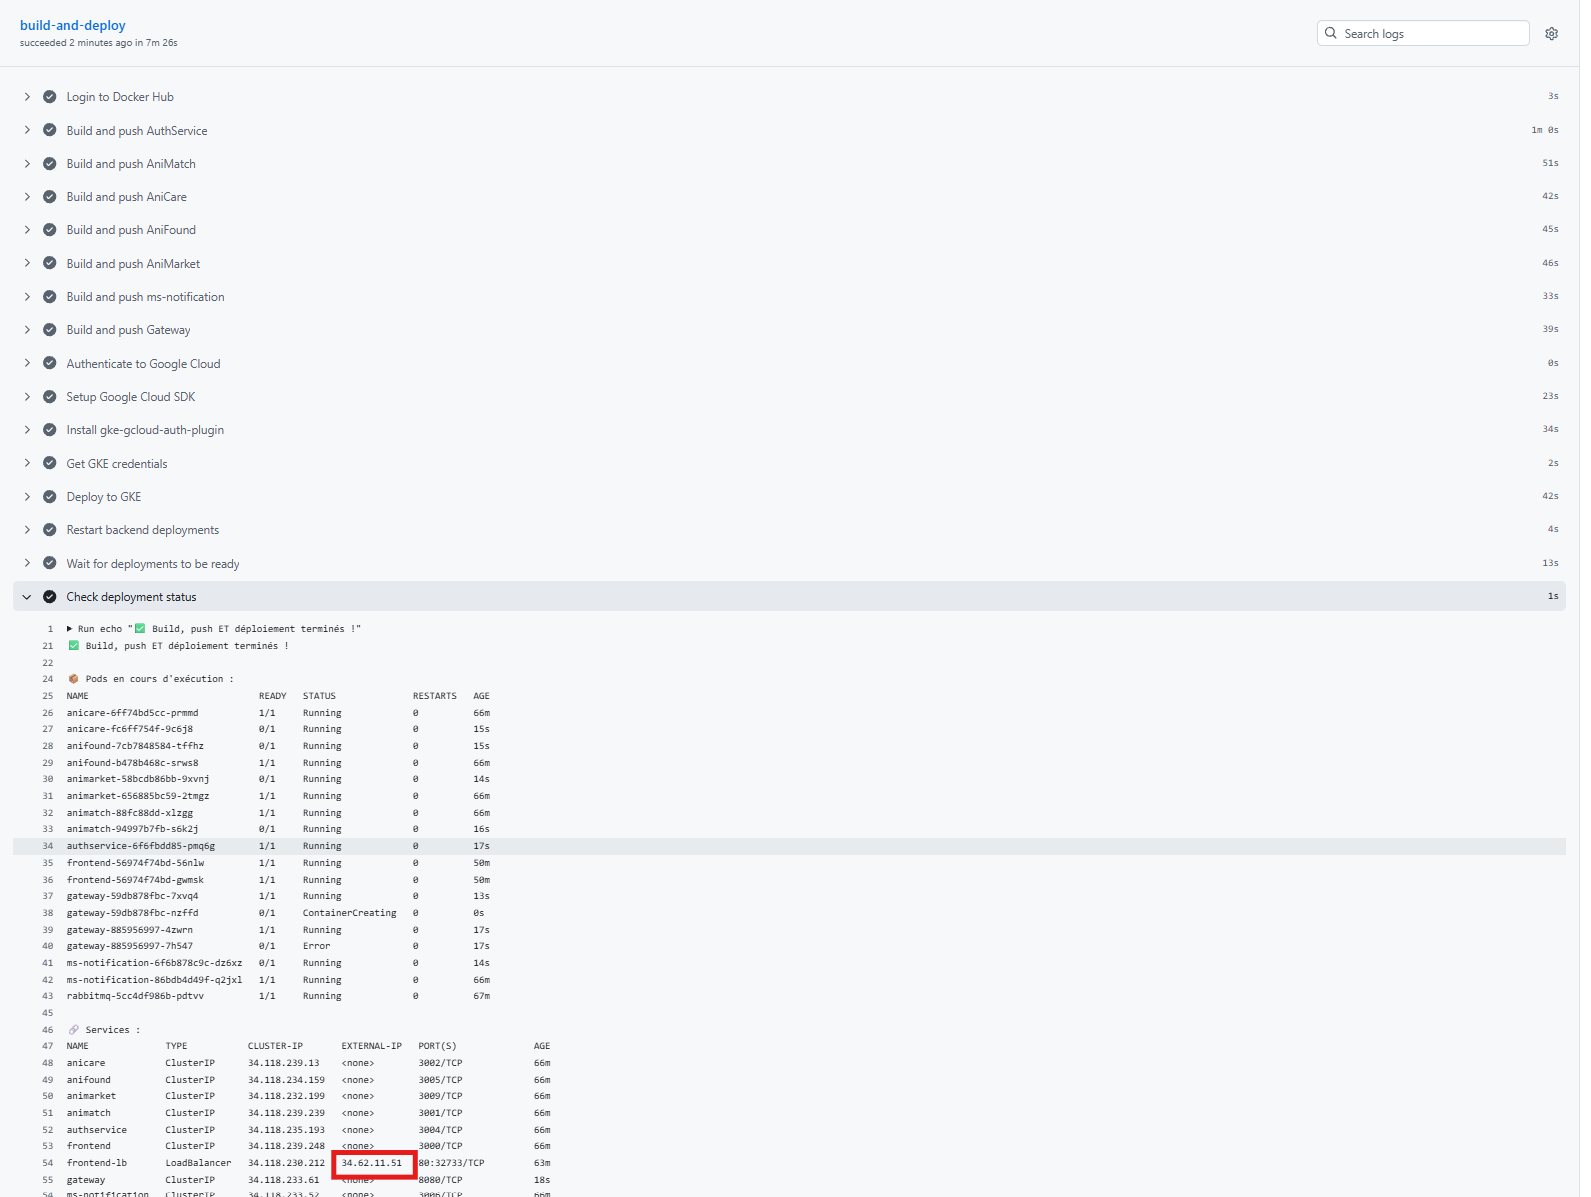
\includegraphics[width=1.3\linewidth]{images/pipeline2.png}
    \caption{Exécution de la pipeline CI/CD dans GitHub Actions}
    \label{fig:execution-ci-cd}
\end{figure} 

\newpage 
\subsection{Monitoring et supervision} 
\subsubsection{Configuration de Prometheus et Grafana sur Kubernetes}

Cette figure illustre le fichier \textbf{monitoring.yml} utilisé pour déployer et configurer Prometheus et Grafana sur Kubernetes afin d’assurer le monitoring des microservices d’AniHub : 
\begin{figure}[H]
    \centering
    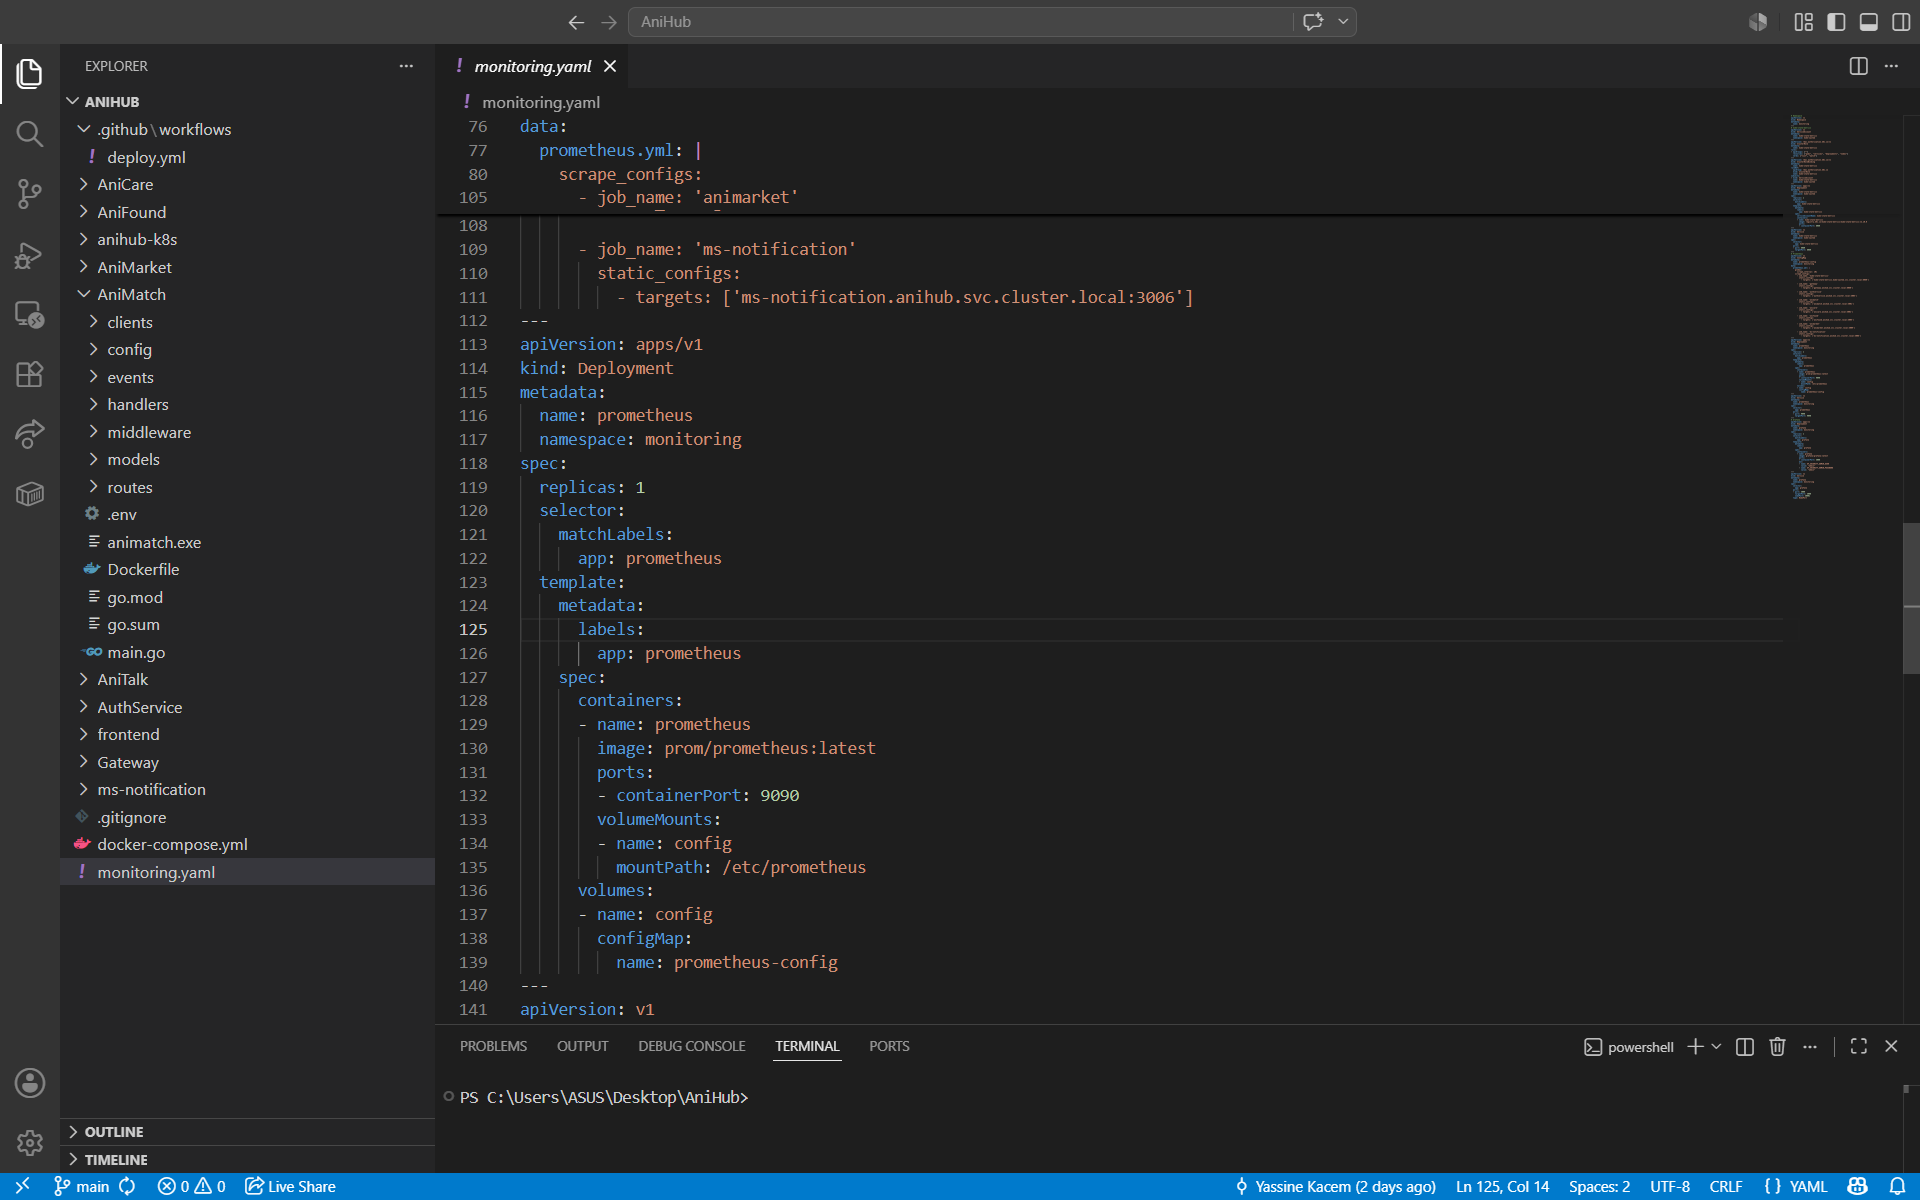
\includegraphics[width=0.4\linewidth]{images/monitoring.yaml.png}
    \caption{Configuration de Prometheus et Grafana sur Kubernetes}
    \label{fig:monitoring-k8s}
\end{figure}  

\subsubsection{Ajout de la route des métriques dans les microservices}

Cette étape permet à Prometheus de collecter les métriques des microservices via la route \texttt{/metrics} afin d’assurer le monitoring de l’application. 
\begin{figure}[H]
    \centering
    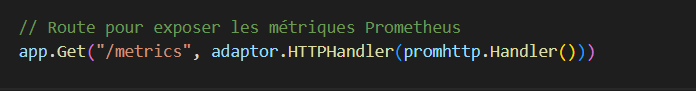
\includegraphics[width=0.6\linewidth]{images/route metric.png}
    \caption{Ajout de la route des métriques dans les microservices}
    \label{fig:metrics-route}
\end{figure} 

\subsubsection{Surveillance des microservices avec Prometheus} 


Cette figure illustre la surveillance des microservices par Prometheus via les targets configurées. Par exemple, le microservice \textbf{gateway} est en état \textbf{UP}, confirmant son bon fonctionnement et la collecte des métriques : 
\begin{figure}[H]
    \centering
    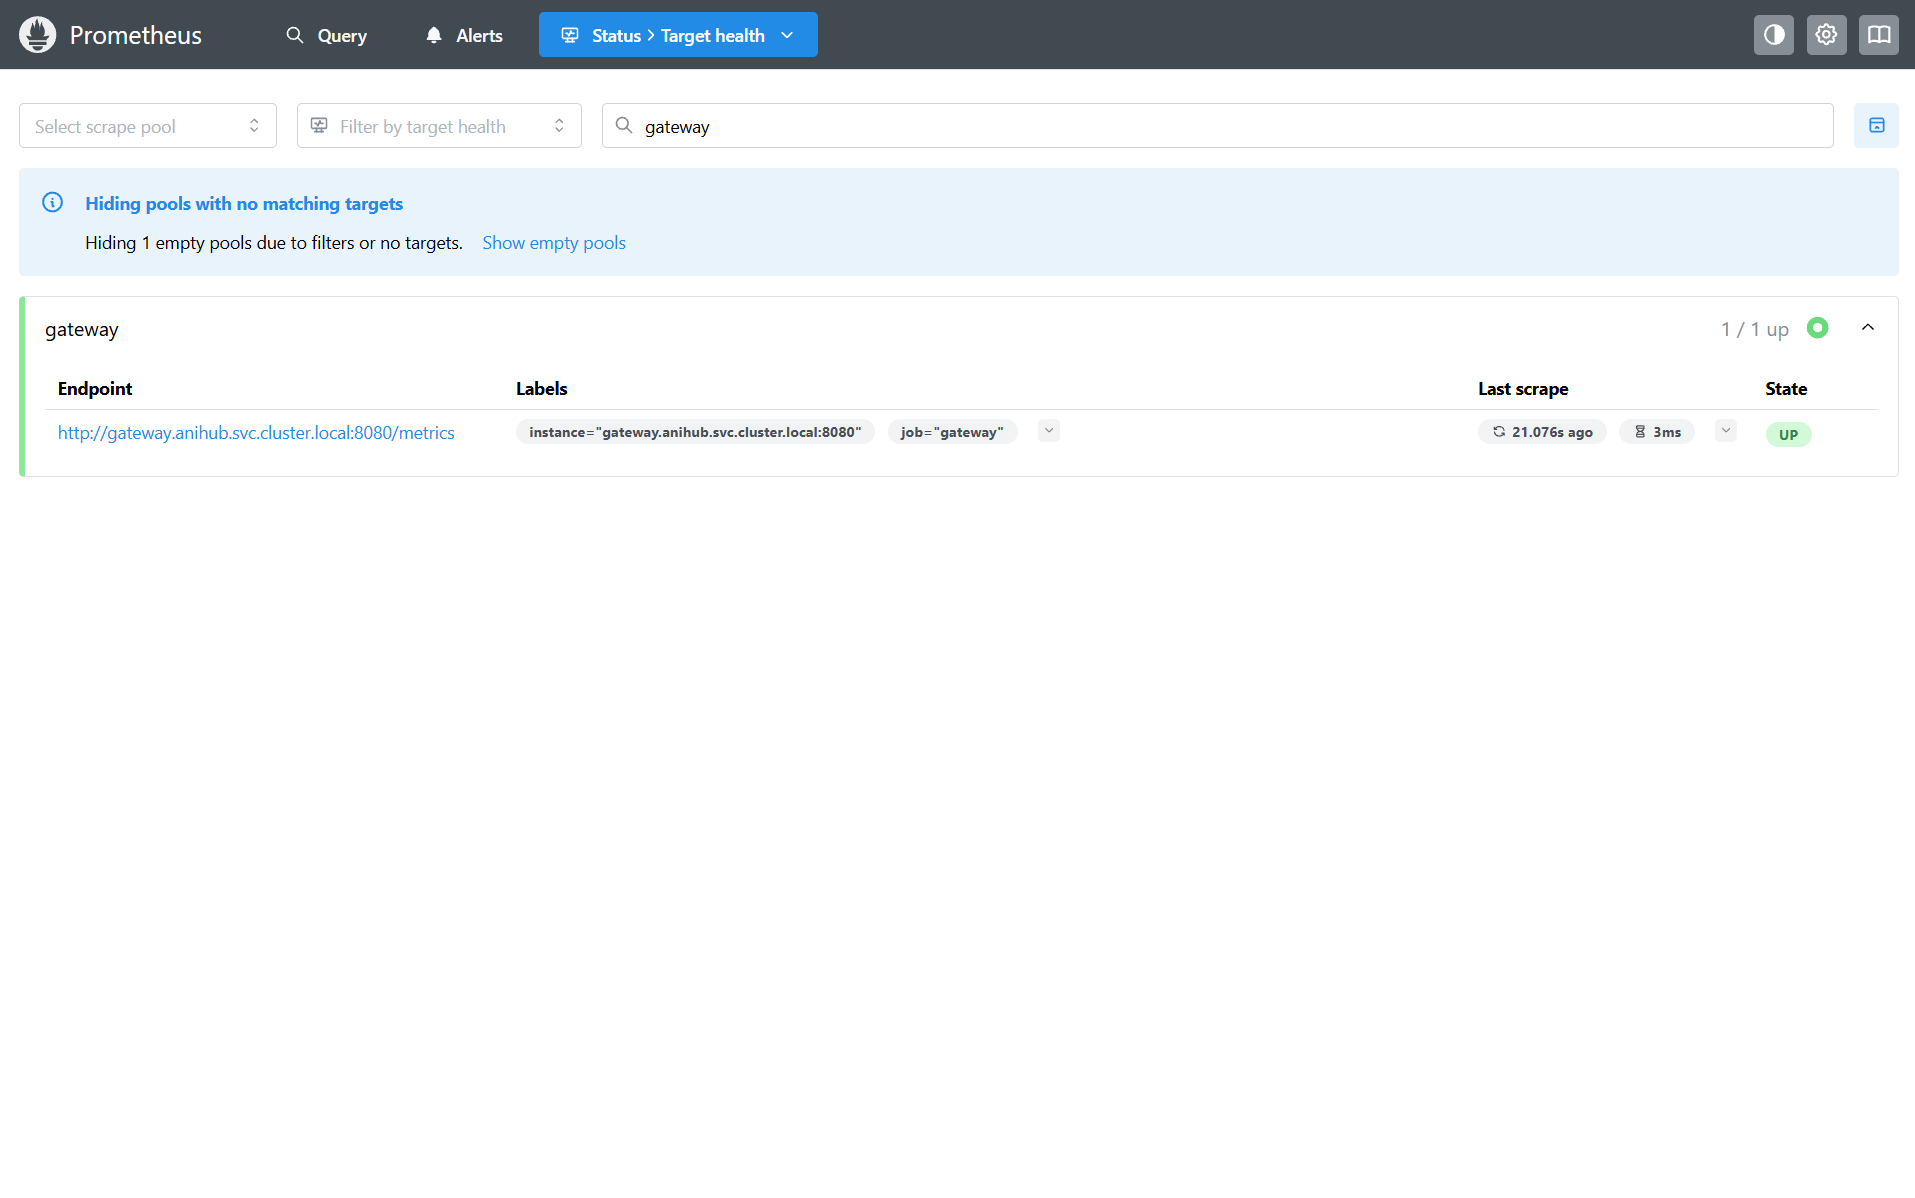
\includegraphics[width=0.5\linewidth]{images/prometheus target.png}
    \caption{Surveillance des microservices avec Prometheus}
    \label{fig:prometheus-monitoring}
\end{figure}
\newpage  
\subsubsection{Page de connexion de Grafana}

Cette figure illustre la page de connexion de Grafana permettant d’accéder à l’interface de monitoring des microservices et du cluster Kubernetes d’AniHub 
\begin{figure}[H]
    \centering
    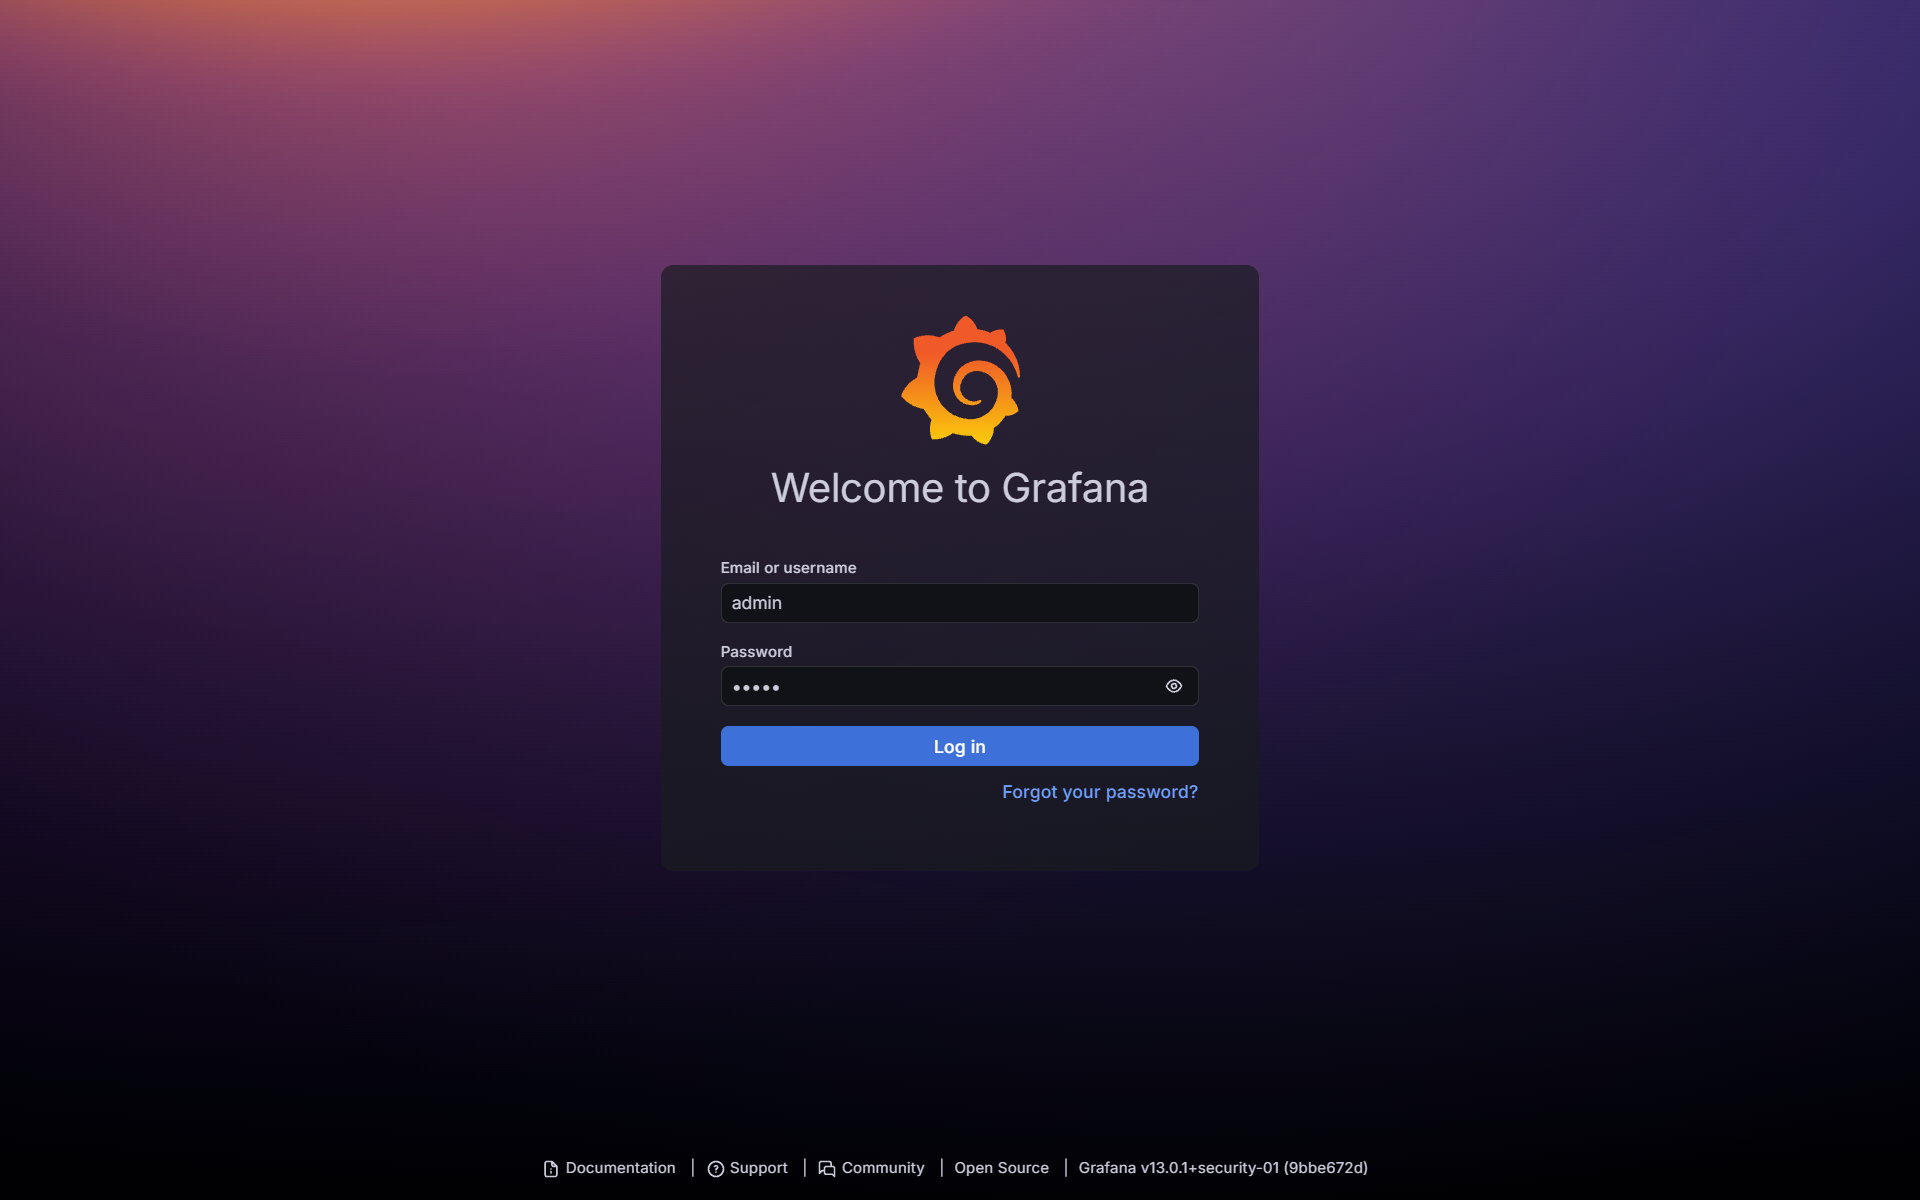
\includegraphics[width=0.6\linewidth]{images/grafana login.png}
    \caption{Page de connexion de Grafana}
    \label{fig:grafana-login}
\end{figure}  

\subsubsection{Tableau de bord Grafana : état de santé des microservices AniHub} 
Cette figure illustre un tableau de bord Grafana affichant l’état de santé des microservices d’AniHub : 
\begin{figure}[H]
    \centering
    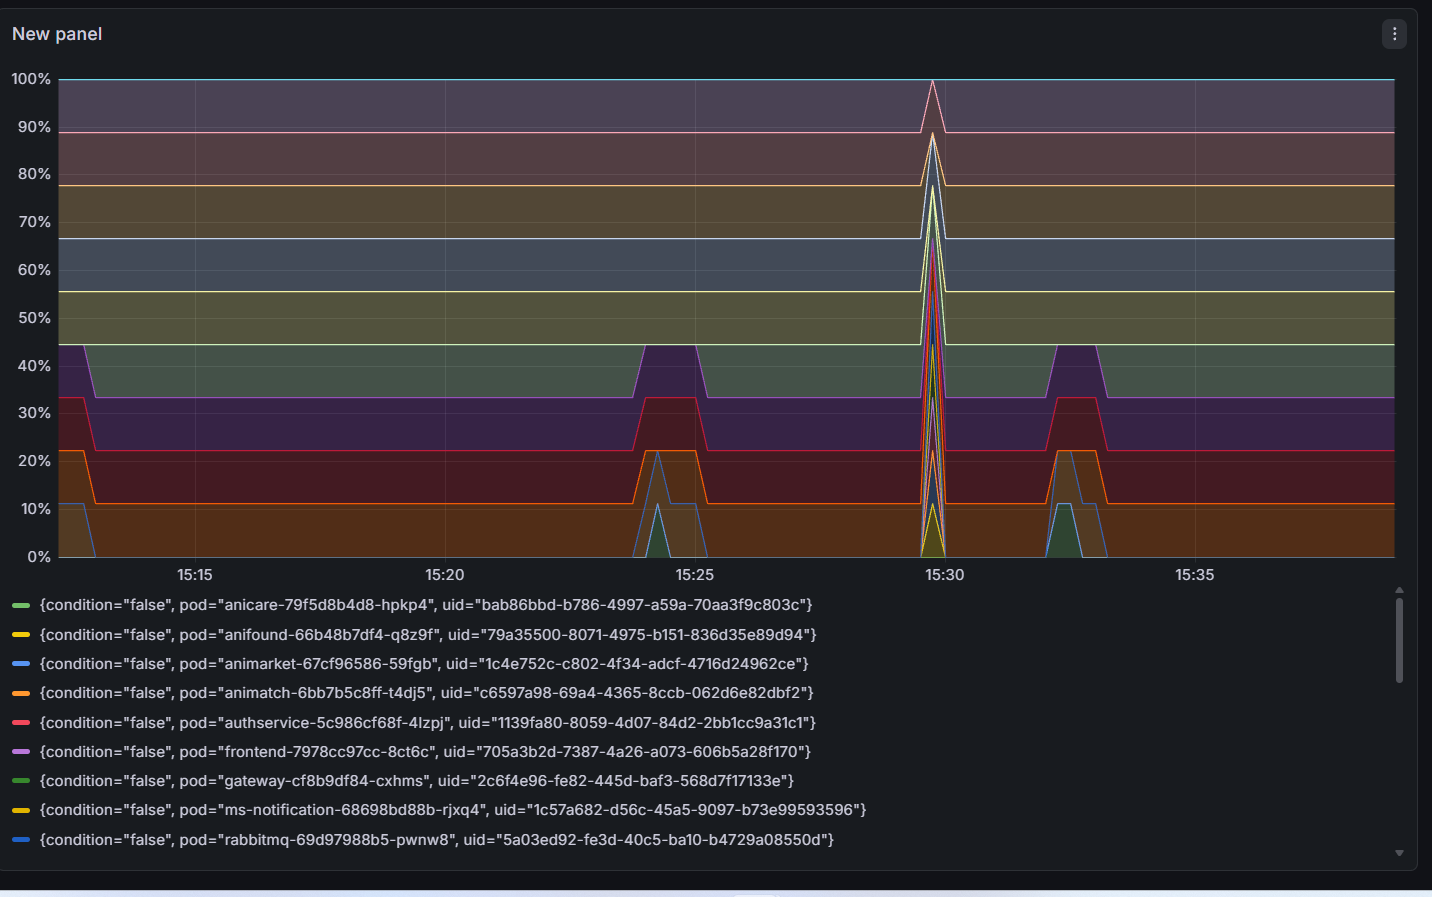
\includegraphics[width=0.9\linewidth]{images/etat de santé des microservices anihub grafana.png}
    \caption{Tableau de bord Grafana : état de santé des microservices AniHub}
    \label{fig:grafana-dashboard}
\end{figure} 
\newpage  


\subsubsection{Tableau de bord Grafana : Utilisation de la mémoire vive (RAM) par pod} 
Cette figure illustre la quantité de mémoire vive (RAM) actuellement consommée par chaque pod du namespace anihub, exprimée en octets : 
\begin{figure}[H]
    \centering
    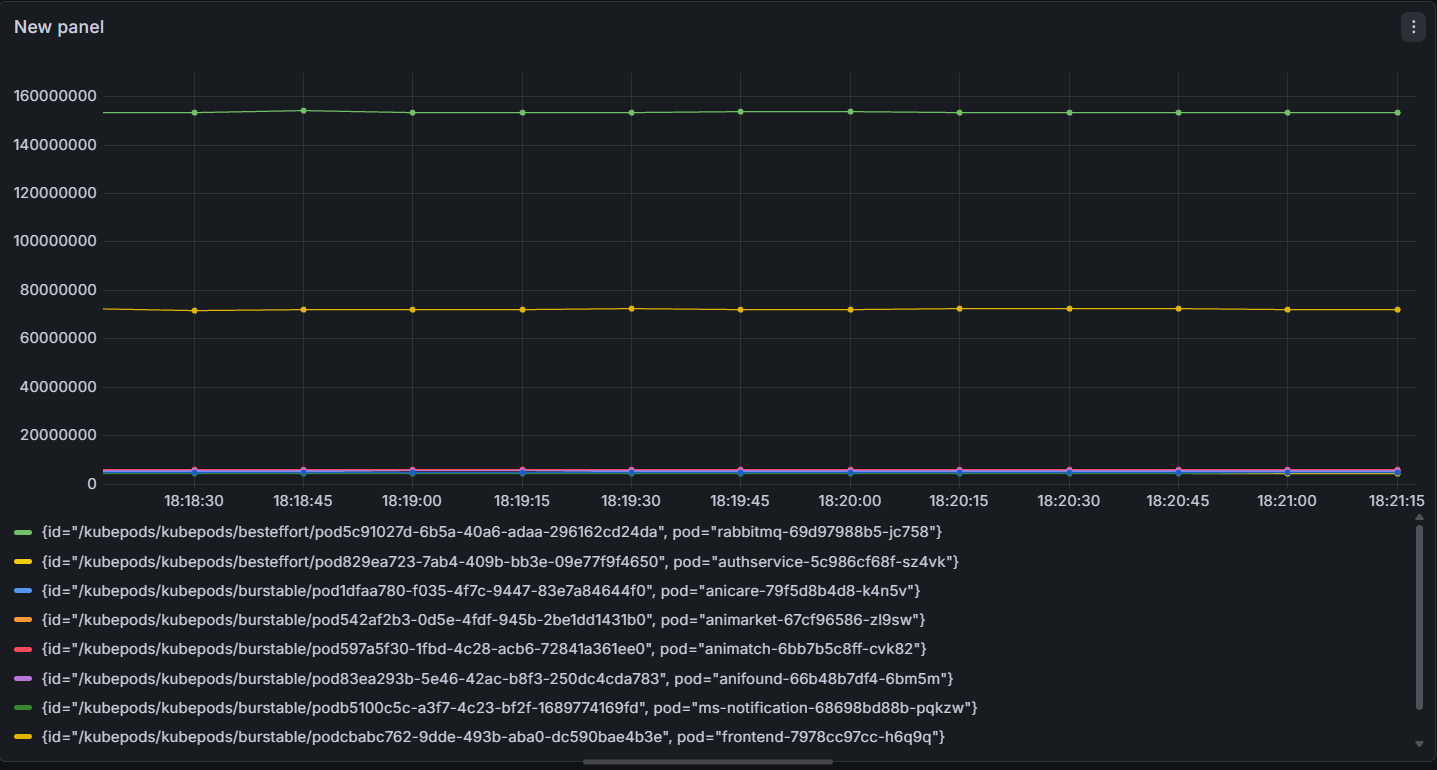
\includegraphics[width=0.8\linewidth]{images/consommation memoire ram.png}
    \caption{Tableau de bord Grafana : Utilisation de la mémoire vive (RAM) par pod}
    \label{fig:ram-usage}   
\end{figure}

\subsubsection{Tableau de bord Grafana : Consommation CPU des microservices AniHub} 
Cette figure illustre le taux d’utilisation du CPU par les microservices de la plateforme AniHub : 
\begin{figure}[H]
    \centering
    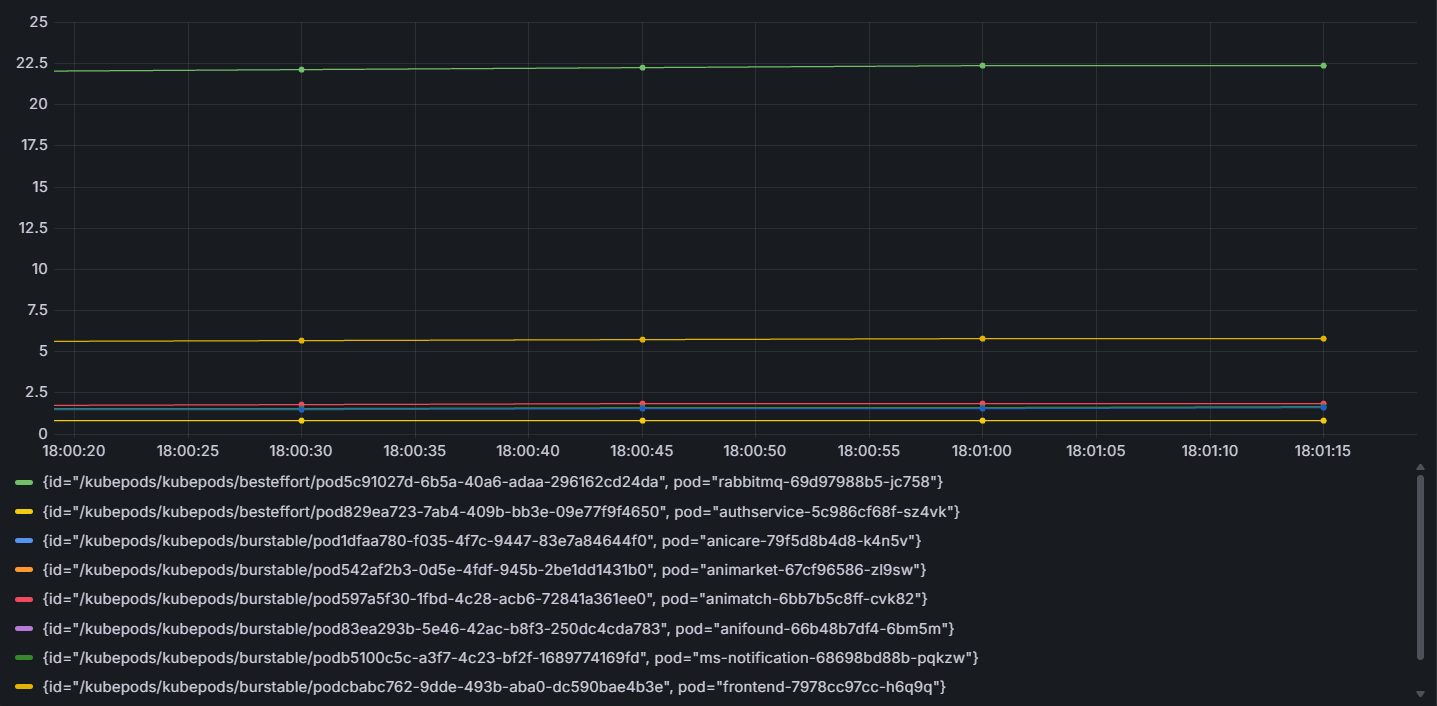
\includegraphics[width=0.8\linewidth]{images/consommation cpu.png}
    \caption{Tableau de bord Grafana : Consommation CPU des microservices AniHub}
    \label{fig:cpu-usage}   
\end{figure} 
\newpage

\subsubsection{Tableau de bord Grafana : Nombre de conteneurs actifs} 
Cette figure affiche le nombre total de conteneurs actuellement en cours d’exécution dans le namespace anihub. Au début, le nombre de conteneurs était de 9. Ensuite, afin de tester le mécanisme de scalabilité, le nombre de réplicas a été modifié à 2, ce qui a entraîné l’augmentation du nombre total de conteneurs à 18 : 
\begin{figure}[H]
    \centering
    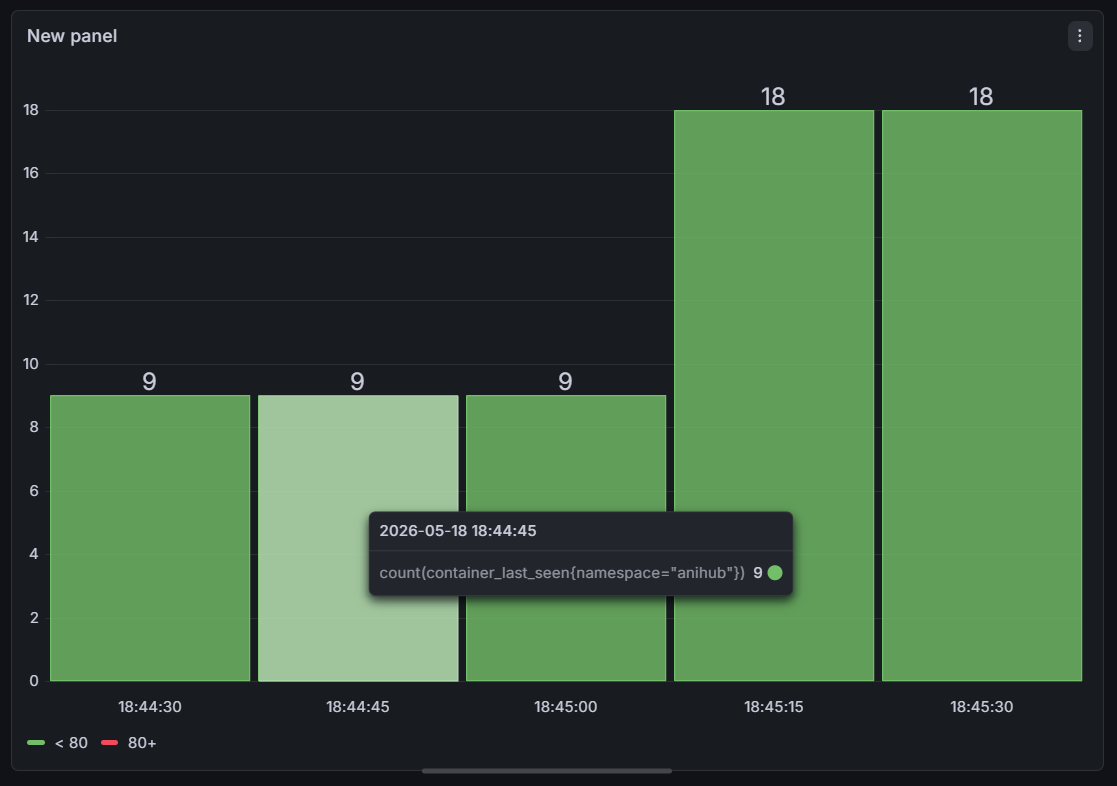
\includegraphics[width=0.7\linewidth]{images/Compteur de conteneurs actifs.png}
    \caption{Tableau de bord Grafana : Nombre de conteneurs actifs}
    \label{fig:containers-active}
\end{figure} 
\subsubsection{Tableau de bord grafana : État de santé de la Gateway} 
Cette figure illustre l’état de fonctionnement instantané de la Gateway, indiquant si elle est active ou indisponible à un instant donné : 
\begin{figure}[H]
    \centering
    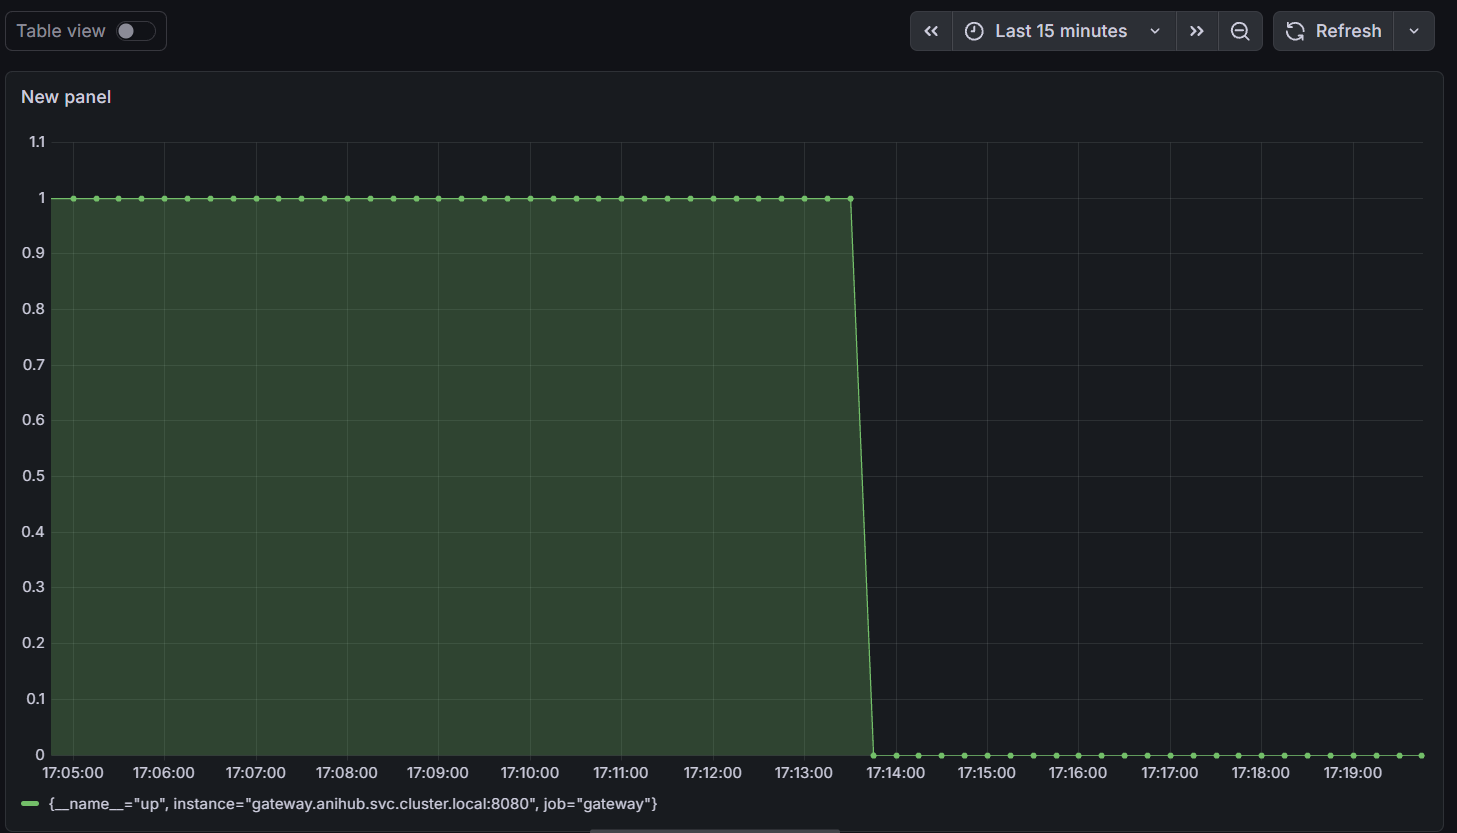
\includegraphics[width=0.7\linewidth]{images/etat de santé gateway.png}
    \caption{Tableau de bord Grafana : État de santé de la Gateway}
    \label{fig:gateway-health}
\end{figure}



\newpage
\subsubsection{Tableau de bord Grafana : Nombre de requêtes du microservice AniMatch} 
Cette figure illustre le nombre de requêtes HTTP du microservice AniMatch sur les deux dernières minutes, réparties selon les méthodes GET, POST, PUT et DELETE, afin d’analyser son activité et sa charge : 
\begin{figure}[H]
    \centering
    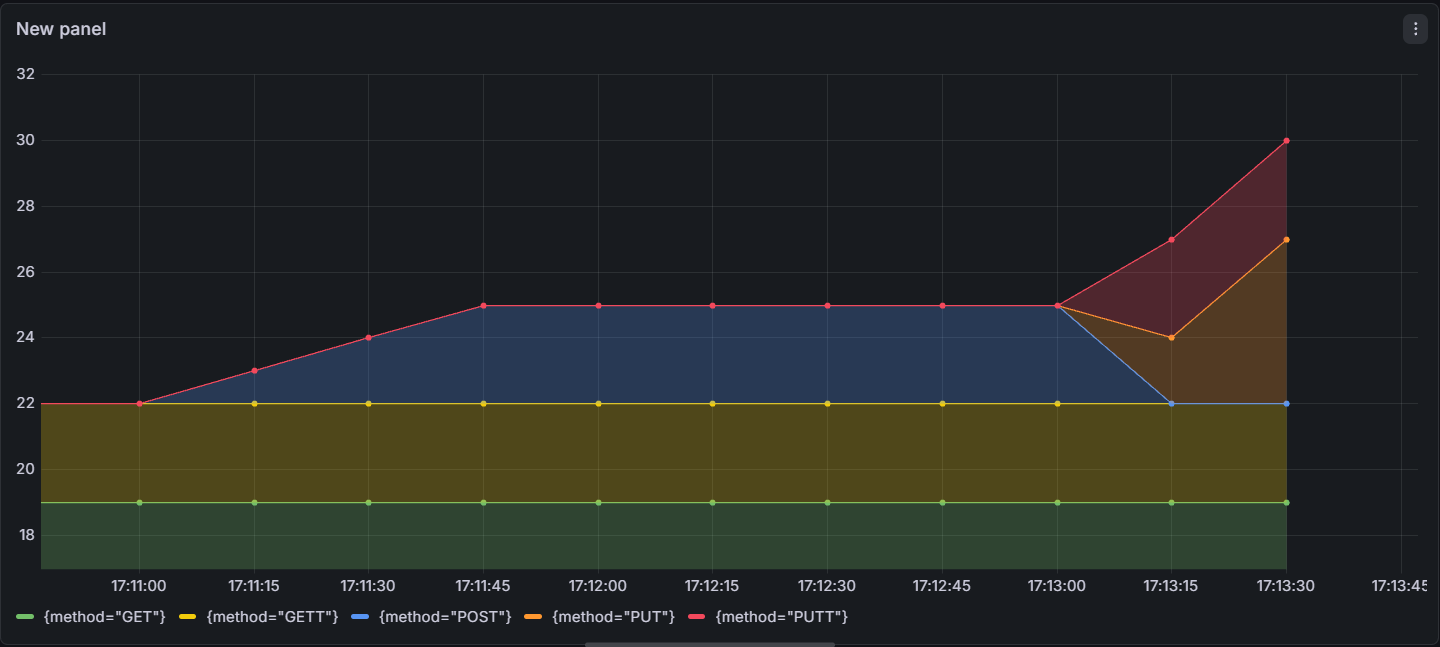
\includegraphics[width=0.9\linewidth]{images/nb requests vers animatch.png}
    \caption{Nombre de requêtes du microservice AniMatch(GET, POST, PUT, DELETE)}
    \label{fig:requests-animatch}
\end{figure}    
\subsubsection{Tableau de bord Grafana :Nombre de requêtes par microservices}
Cette figure illustre le nombre de requêtes traitées par chaque microservice de l’application AniHub, permettant d’analyser la charge et l’activité de chaque service : 

\begin{figure}[H]
    \centering
    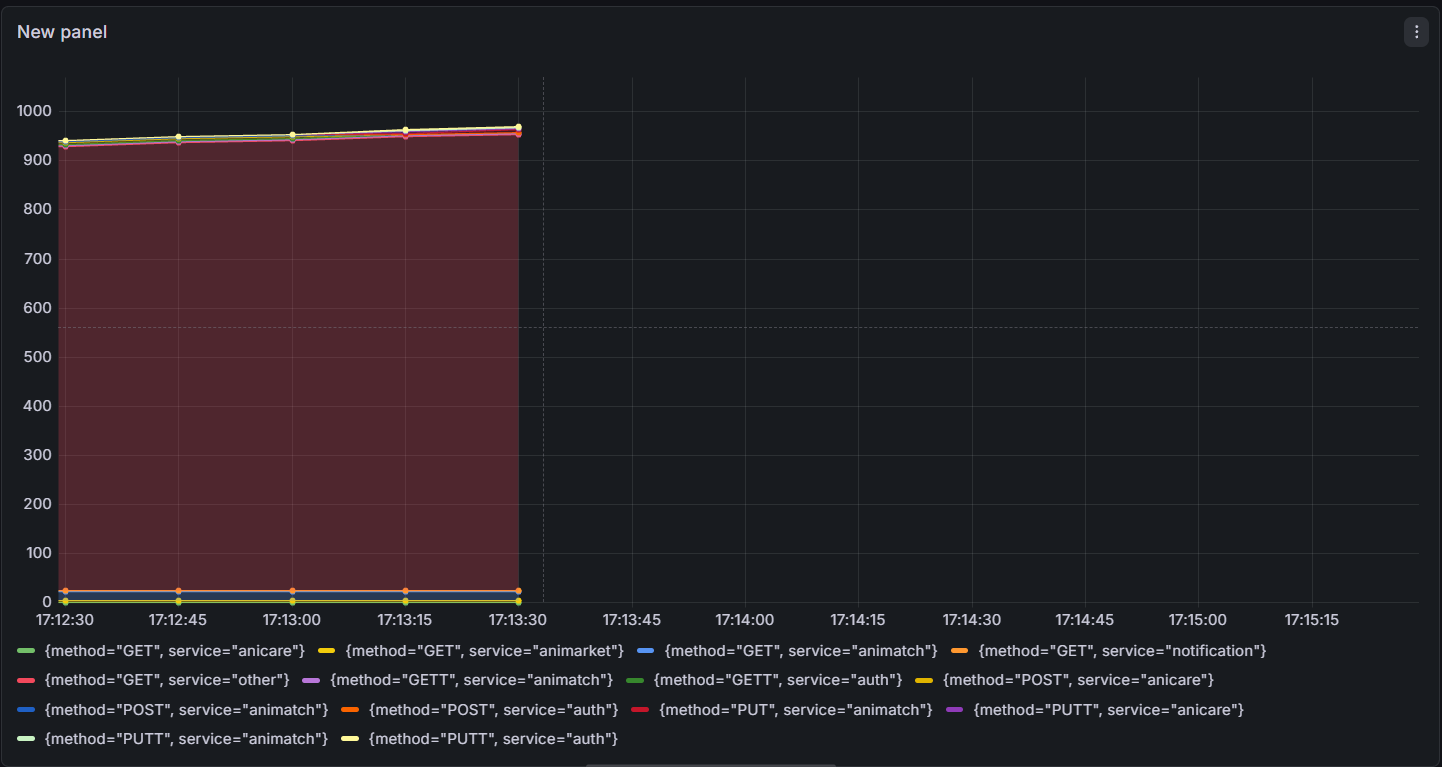
\includegraphics[width=0.9\linewidth]{images/nb requetes de services.png}
    \caption{Nombre de requêtes par microservices}
    \label{fig:requests-microservices}
\end{figure} 
\newpage






